\chapter{Meter inference and tracking}\label{chap:meterInfTrack}
\begin{epigraphs}
  \qitem{...the first beat (sam) is highly significant structurally, as it frequently marks the coming together of the rhythmic streams of soloist and accompanist, and the resolution point for rhythmic tension.}{\citeA[p. 81]{clayton:00:time}}
\end{epigraphs}
\noindent Meter analysis \index{Meter analysis} of audio music recordings is an important \gls{MIR} task. It provides useful musically relevant metadata not only for enriched listening, but also for pre-processing of music for several higher level tasks such as section segmentation, structural analysis and defining rhythm similarity measures. 

To recapitulate, meter analysis aims to time-align a piece of audio music recording with several defined metrical levels such as tatum, tactus, measure (bar). In addition, it also tags the recording with additional meter and rhythm related metadata such as time signature, median tempo and salient rhythms in the recording. Within the context of Indian music, meter analysis aims to time-align and tag a music recording with \gls{tala} related events and metadata. 

This chapter aims to address some of these important tasks related to meter analysis within the context of Indian art music, presenting several approaches and a comprehensive evaluation of those approaches. The main aims of the chapter are: 
\begin{enumerate}[leftmargin=*]
 \item To address meter analysis tasks for the music cultures under study - Carnatic and Hindustani music. The tasks of meter inference, meter tracking and informed meter tracking are addressed in detail to formulate these tasks and propose several approaches to address the tasks. 
 \item To present a detailed description of the state of the art and the proposed Bayesian models and inference schemes for meter analysis. 
 \item To present an evaluation of the state of the art meter tracking approaches based on Bayesian models and explore extensions to those approaches, for the rhythm annotated datasets of Carnatic and Hindustani music. A comprehensive performance analysis is presented for these approaches, identifying their strengths and limitations for the tasks under study. 
\end{enumerate}
%
\section{The meter analysis tasks}
We describe the meter analysis tasks addressed in this dissertation, from the least informed to the most informed. This order of tasks also emphasizes different practical scenarios for such tasks, and hence the results can indicate the type of task and the additional information to be provided to achieve the level of performance required for an application. We will also describe how the set of tools and approaches described in the chapter can be adapted and used in each of these tasks, making the task of meter analysis flexible to the available audio data and the related additional metadata. We continue and elaborate building on the formulation presented in \secref{sec:probdef:thesismeter}. 
\subsubsection{Meter inference}
Given an audio music recording, meter inference\index{Meter inference} aims to estimate the rhythm class (or meter type or \gls{tala}), possibly time-varying tempo, beats and downbeats. In the context of Carnatic music, the task of meter inference aims to recognize the \gls{tala}, estimate the time varying tempo ($\iai$ or $\ibi$), the beat locations and the \gls{sama} (downbeat) locations. Since some of the beats correspond to the \gls{anga} boundaries, with the \gls{sama} and numbered beat locations (beat number in the cycle), the \gls{anga} (section) boundaries can be indirectly inferred, e.g. the beats 1 (\gls{sama}), 5, 7 mark the start of the three sections of the \gls{adi} \gls{tala}. Similarly, for Hindustani music, meter inference task aims to recognize the \gls{taal}, estimate the time varying tempo ($\ibi$), the \gls{matra} and the \gls{sam} locations. With the numbered \gls{matra} and \gls{sam} locations, the \gls{vibhaag} boundaries can be indirectly inferred, e.g. the \glspl{matra} 1 (\gls{sam}), 3, 6, 8 indicate the start of the four sections in \gls{jhaptal}. For Carnatic music, in addition to the beats, we can also estimate the subdivision \glspl{akshara}, which can be grouped into beats. 

Without any prior information on metrical structure, meter inference is a difficult task owing to the large range of tempi and different \glspl{tala}. The problem is further made harder due to several \glspl{tala} having similar structure. In Carnatic music, it is quite possible that the same composition can be performed in two different \glspl{tala}, which further can lead to confusion, e.g. the compositions in \gls{rupaka} \gls{tala} (12 \glspl{akshara} in a cycle) can be performed in \gls{tishra} \gls{nade} \gls{adi} \gls{tala} (24 \glspl{akshara} in a cycle, see \figref{fig:taala:aditishra}). A common example is the composition Himadri Suthe\footnote{\url{https://musicbrainz.org/work/6155262b-601a-41ba-8dcf-6f5b15b744f6}} in \gls{raga} Kalyāṇi. 

From a practical application point of view, most of commercially released music in both Carnatic and Hindustani music has the name of the \gls{tala} as a part of the editorial metadata, and hence \gls{tala} recognition is a redundant task. Even within a live concert, the musician announces the \gls{tala} of the piece, or shows it with hand gestures in Carnatic music. Meter inference is used as a baseline task to understand the complexity of uninformed meter analysis. 
\subsubsection{Meter tracking}
Given that the \gls{tala} of an audio music piece is often available as editorial metadata, the most relevant meter analysis task for Indian art music is meter tracking\index{Meter tracking}. Given an audio music recording and the rhythm class (or meter type or \gls{tala}) of the music piece, meter tracking aims to estimate the time varying tempo, the beat and the downbeat locations. In the context of Carnatic music, meter tracking aims to track the time varying tempo, beats and the \gls{sama} from an audio music recording, given the \gls{tala}. For Hindustani music, given the \gls{taal}, the task aims to track the time varying tempo ($\ibi$), the \gls{matra} and \gls{sam}. The section boundaries of the \gls{tala} can be indirectly inferred as explained earlier. 

Assuming that the \gls{tala}, and hence the metrical structure is known in advance is a fair and practical assumption to make, we explore if providing this information helps to track the metrical structure better. Meter tracking is the main problem and the most comprehensively addressed task in this thesis. We explore different approaches and evaluate them on the rhythm annotated datasets of Carnatic and Hindustani music. The proposed novel extensions and enhancements are also evaluated for the task of meter tracking. 
\subsubsection{Informed meter tracking}
Informed meter tracking is a sub-task of meter tracking in which some additional information apart from the meter type is provided along with the audio recording. The additional information could be in the form of a tempo range, a few instances of beats and downbeats annotated, or even partially tracked metrical cycles. These additional metadata could come from manual annotation or as an output of other automatic algorithms, e.g. the median tempo of a piece can be obtained from a standalone tempo estimation algorithm, or some melodic analysis algorithms might output (with a high probability) some beats/downbeats as a byproduct. 

From a practical standpoint, it is useful to explore informed meter tracking. While it is prohibitively resource intensive to manually annotate all the beats and downbeats of a large music collection, it might be possible to seed the meter tracking algorithms with the first few beats and downbeats, which could improve meter tracking performance. For a musician or even an expert listener, it would be very easy to tap some instances of the beat and \gls{sama}, which could then be used automatically track meter, which is a useful application. 

We aim to explore these questions, to see whether providing additional higher level information improves meter tracking performance. In specific, we explore two variants of informed meter tracking: 
\begin{enumerate}[leftmargin=*]
    \item Tempo-informed meter tracking in which the median tempo of the piece is provided as an additional input to the meter tracking algorithm. Providing the median tempo is hypothesized to help reduce tempo octave errors - tracking the metrical cycles at the correct metrical level instead of tracking half and double cycles. The median tempo can be obtained through simpler state of the art tempo estimation algorithms outlined in \secref{sec:bkgnd:tempoest} (one such algorithm for Carnatic music is also described later in this chapter in \secref{sec:metertrack:dp}). Since the tempo of a piece can vary over time, a narrow range of tempo for the piece can also be provided in addition or in lieu of the median tempo. 
    \item Tempo-sama-informed meter tracking in which the median tempo and the first downbeat location in the excerpt are provided as additional inputs to the meter tracking algorithm. The practical scenario for such a case is a semi-automatic meter tracking system, where a human listener can tap along to the first one (or few) downbeats of the piece and an automatic meter tracker would then track the rest of the piece. In this thesis, we only explore the use of first downbeat of the piece in informed meter tracking.
\end{enumerate}
% 
There are other meter analysis tasks that have been addressed in \gls{MIR}, such as beat tracking, and downbeat tracking from the set of known beats. The task of beat tracking as defined in the state of art is ill defined in Indian art music, due to possibly non-isochronous pulsation. We can adapt the task and track a uniform pulsation as the beat. However, since the tasks of meter inference and meter tracking aim to track all the relevant events of the metrical cycle, the task of beat tracking is subsumed in those tasks. We do not address the task of beat tracking in Indian music directly, but as a sub-task of the meter tracking/inference tasks. Estimating the downbeats and the start of measure from a set of beats, as done by \citeA{davies:06:downbeat} and \citeA{hockman:12:downbeat} is also handled as a sub-task within the joint estimation of tempo, beats and the downbeats. 

We now describe the approaches to these tasks, starting with some preliminary approaches followed by Bayesian models. With Bayesian models, several different extensions are proposed over the state of the art models. 
%
\section{Preliminary experiments}\label{sec:mt:earlyexpts}
% \note{These are tried to see if just features and some DP is enough to track beats and \gls{sama}. Mainly based on features Pre-2014 work: Onset detection, preliminary experiments on onset detection, HPSS, Akshara pulse tracking, and downbeat estimation (ICASSP 2014).}
The preliminary experiments around the task of meter analysis are exploratory experiments with existing features, rhythm descriptors, methods and algorithms to gain insights into the problem and test their relevance and utility in these tasks. The aim of including them in thesis is to gain useful insights and understand the limitations of those algorithms in meter analysis tasks for Indian art music. Only a selection of them are described here, primarily for Carnatic music, as a base for improved Bayesian models for meter analysis. We proposed a novel meter tracking algorithm in Carnatic music \cite{ajay:14:talaTrack} using pre-existing tools and rhythm descriptors, which is described in detail. The features and tools are explained as a part of the proposed meter tracking algorithm, emphasizing on their utility. 
%
\subsection[Meter tracking using dynamic programming]{Meter tracking using dynamic\\ programming}\label{sec:metertrack:dp}
The primary philosophy of meter tracking is to incorporate specific knowledge of the rhythmic structures we aim to estimate, which is also used in this approach. However, the approach aims to estimate the components of meter separately using a descriptor for each music concept. Using Carnatic music as an illustration, the algorithm estimates the \gls{akshara} period $\iai$, the \gls{akshara} pulse locations, and the \gls{sama}. For estimating these components, a set of rhythm descriptors are first computed from the audio that are indicative of the possible candidates for each musical concept. The periodicity and the relationships between these structures are then utilized to estimate the components. This framework can be generalized to estimating other rhythmic structures by suitably modifying the audio descriptor for the specific music culture and the rhythmic structure under consideration. 
\begin{figure}
  \centering
 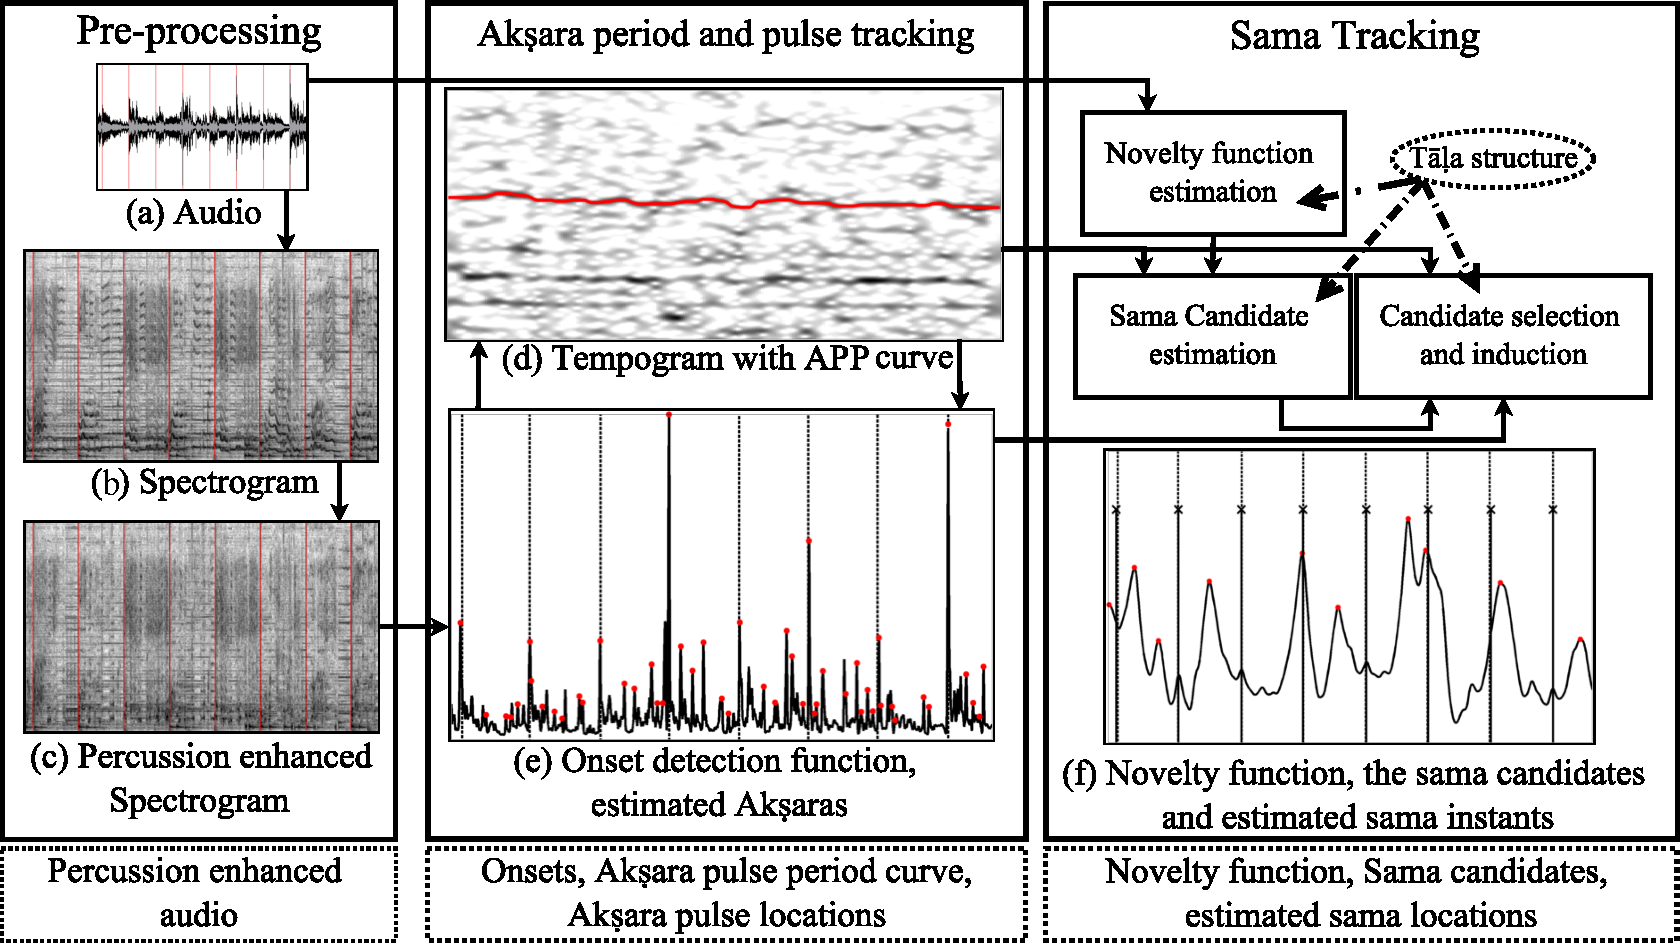
\includegraphics[width=\textwidth]{blockDiags/samaTrack-ICASSP-BlockDiag.pdf}
\caption[Block diagram of the \gls{tala} tracking algorithm proposed by \protect\citeA{ajay:14:talaTrack}]{Block diagram of the algorithm showing the signal flow and representative illustrations of different stages of the algorithm. The important outputs at each stage are also shown at the bottom. In each panel, the vertical lines that run through the panel indicate the \gls{sama} ground truth instants. The estimated \gls{sama}/\gls{akshara} candidates are shown with red dots and the estimated \gls{sama} are shown with $\times$.}\label{fig:BD:samaTrackICASSP}
\end{figure}

The algorithm for Carnatic music is explained in detail in this section. A hypothesis is that the \gls{akshara} pulses can be estimated from the onsets of mridangam, and hence a percussion onset based rhythm descriptor \cite{bello:05:onset} is useful for tracking the \gls{akshara} pulses. Tempogram\index{Tempogram}, a mid-level tempo representation for music signals proposed by \citeA{grosche:11:tempogram} is used to track the time-varying \gls{akshara} period. A novelty function\index{Novelty function} is computed using a self similarity matrix constructed using frame level onset and timbral features. These are then used to estimate possible \gls{akshara} and \gls{sama} candidates, followed by a candidate selection based on periodicity constraints, which leads to the final estimates. A block diagram of the approach is shown in \figref{fig:BD:samaTrackICASSP}. The features and the approach are explained further in detail. 
%
\subsubsection{Pre-processing: Percussion enhancement}
\begin{figure}
\captionsetup[subfigure]{labelformat=empty}
\centering
    \subfloat[]{\label{fig:preproc:hpssorg}
      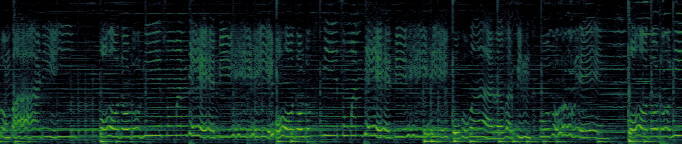
\includegraphics[width=0.95\textwidth]{meterTrack/HPSS-org.png}
    } \\ \vspace{-2em}
    \subfloat[]{\label{fig:preproc:hpssen}
      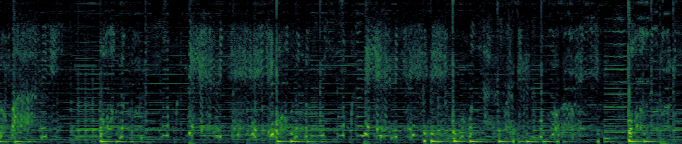
\includegraphics[width=0.95\textwidth]{meterTrack/HPSS-enhanced.png}
    } 
\caption[An illustration of percussion enhancement]{An illustration of percussion enhancement on a short audio excerpt of Carnatic music. The figure shows the spectrogram of the audio excerpt, before percussion enhancement (top panel) and after percussion enhancement by suppressing the lead melody (bottom panel). The lead melody is suppressed, while the \gls{tambura} (drone) is still present.}\label{fig:preproc:hpss}
\end{figure}
The \gls{akshara} pulse most often coincides with the onsets of mridangam strokes. To enhance the mridangam onsets, percussion enhancement is performed on the downmixed mono audio signal $\signal$ obtained from a music piece $\songVar$, as it has been shown to improve beat tracking performance in pieces with predominant vocals by \citeA{zapata:13:beatVS}. The predominant melody (\fzero)\index{Fundamental frequency} is estimated using the algorithm proposed by \citeA{salamon:12:melody} using which the harmonic component of the signal is extracted using a sinusoidal+residual model proposed by \citeA{serra:97:sms}. The percussion enhanced signal $\percsignal$, with the harmonic component suppressed, is used for further processing (\figref{fig:BD:samaTrackICASSP}(c)). An illustration of percussion enhancement for a short audio excerpt of Carnatic music is shown in \figref{fig:preproc:hpss}. 
%
\subsubsection{\Gls{akshara} period and pulse tracking}
\index{Tempo tracking}The spectrogram of $\percsignal$ is used to compute two frame level spectral flux\index{Spectral flux} based onset detection\index{Onset detection} functions \cite{bello:05:onset} computed every 11.6 ms. For each audio frame $k$ ($k \leq \nframes$), the first function ($\odfspfull$) uses the whole frequency range of the spectrogram and the other function computes the spectral flux only in the range of $0-120$ Hz ($\odfsplow$) and captures the low frequency onsets of the left (bass) drum head of the mridangam. 

The function $\odfspfull$ is used to compute a Fourier-based Tempogram $\tgMat$ proposed by \cite{grosche:11:tempogram}, computed every 0.25 second using a 8 second long window (\figref{fig:BD:samaTrackICASSP}(d)). If the time indexes at which the tempogram is computed is denoted with $i$, $(1\leq i \leq \nTGframes)$, the most predominant $\iai$ curve can be tracked by estimating the best path $\Gamma = \{\gamma_i: i = 1,2, \cdots, \nTGframes\}$ through the tempogram matrix $\tgMat$ that provides a balance between tempogram amplitude at time index $i$, $\tgMat_{\gamma_{_{i}},i}$, and the local continuity of $\iai$. An objective function, that is an extended version of the one used by \citeA{wu:11:beatDP}, is defined as shown in \eqnref{eqn:iai:icassp14}. 
%
\begin{equation}\label{eqn:iai:icassp14}
J_{1}\left(\Gamma,\theta_{1},\theta_{2}\right)=\underset{i=1}{\overset{\nTGframes}{\sum}}\tgMat_{\gamma_{_{i}},i}-\underset{i=1}{\overset{\nTGframes-1}{\sum}}\left(\theta_{1}\left|\gamma_{i}-\gamma_{i+1}\right|+\theta_{2}\;\Osym\left(\frac{\gamma_{i}}{\gamma_{i+1}}\right)\right) 
\end{equation}
The function $\Osym(\gamma_i/\gamma_{i+1})$ is an extra penalty term to penalize tempo doubling and halving between adjacent frames, and the parameters $\theta_1$ $(= 0.01)$ and $\theta_2$ $(= 10^6)$ provide different weights to the three terms. Based on observations from the \acrshort{CMDf} dataset, the search for the best path through the tempogram is restricted between the range of 120 to 600 APM (\glspl{akshara} per minute). 

The above objective function is solved using a \gls{DP} based approach to obtain a $\iai$ curve. Assuming the longest tracked $\iai$ curve to be at the correct metrical level, any possible tempo doubling/halving errors that are present are corrected to obtain the final curve $\Gamma^\optstar$ (\figref{fig:BD:samaTrackICASSP}(d), $\Gamma^\optstar$ is shown as a thick red line). Using the $\iai$ and the \gls{tala} information, we can obtain the time varying $\isi$ curve for the piece by multiplying the $\iai$ by the number of \glspl{akshara} in a cycle of the \gls{tala}. A further example of a tempogram and the estimated time varying $\iai$ curve for a piece of Carnatic music\footnote{Kamalamba, a \gls{kriti} in \gls{raga} Ānandabhairavi and \gls{mishra chapu} \gls{tala}, from the album Madrasil Margazhi 2005 by Aruna Sairam: \url{http://musicbrainz.org/recording/3baa722d-480e-4ae7-8559-a88dce41e1d4}} from \acrshort{CMDf} dataset is shown in \figref{fig:tempogram:app}. The figure shows the variations in tempo through a Carnatic music piece.
\begin{figure}
\centering
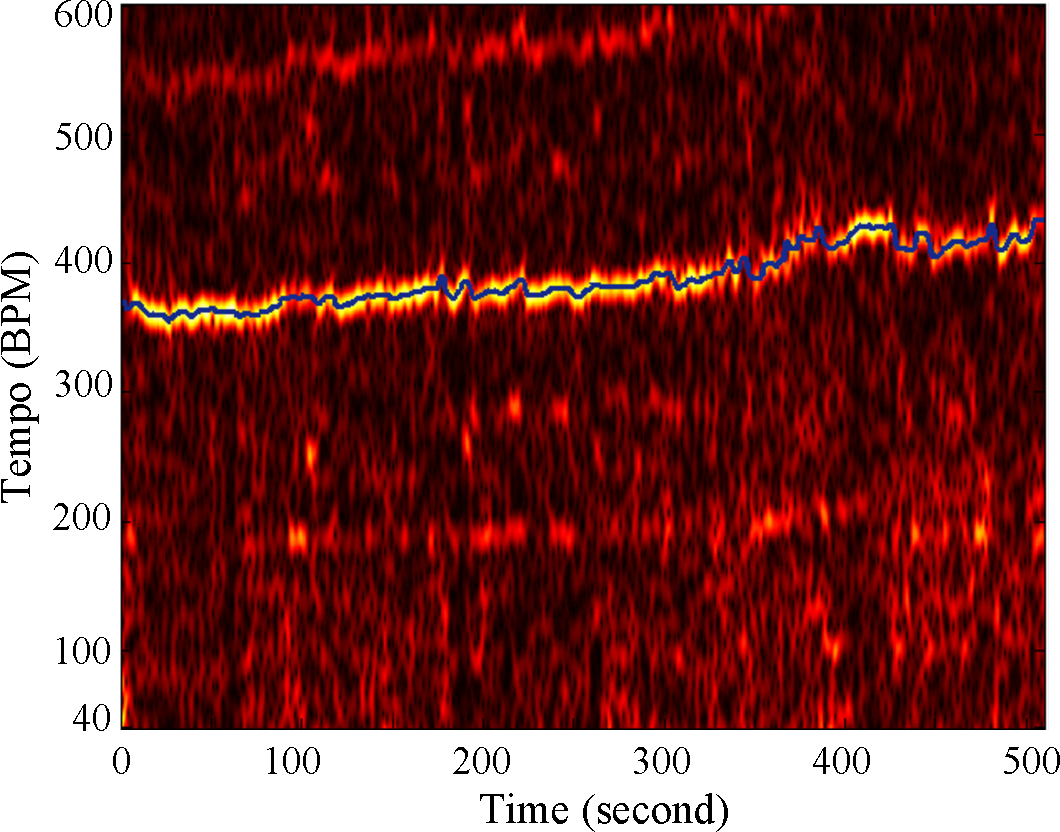
\includegraphics[scale=0.55]{meterTrack/tempogram-APP.pdf}
\caption[Estimated time varying tempo curve with tempogram]{Estimated time varying tempo curve (shown as a bold blue line) plotted on top of a tempogram, for a Carnatic music piece. In the piece, apart the local tempo variations, we can see that the tempo increases with time. The tempogram shows high values in tempo octave related bands, with the highest value (in yellow) at the estimated $\protect\iai$.}\label{fig:tempogram:app}
\end{figure}

The \gls{akshara} pulse locations predominantly lie on strong mridangam onsets. The \gls{akshara} pulse candidates are estimated as the peaks of the function $\odfspfull$. Using these $\kappa$ candidate peaks $\left\{o_i\right\}$, $i=1,2,3,\cdots,\kappa$, with locations $t_{i}$ and peak amplitude $\xi_{i}$, a cost function is setup as shown in \eqnref{eqn:AkCandEst:icassp14} to select the best candidates that provide a balance between the amplitude of these candidates and a periodicity provided by the estimated \gls{akshara} period. The best set of candidates $\aksSet = \left\{o^{\optstar}_i\right\} \subset \left\{o_i\right\}$ are estimated using a \gls{DP} approach (\figref{fig:BD:samaTrackICASSP}(e)).
\begin{equation}
\label{eqn:AkCandEst:icassp14}
J_{2}\left(\{o_{i}\},\delta\right)=\underset{i\subset \{1,2,\cdots, \kappa\}}{\sum}\left(\xi_{i}+\delta \, \Upsilon(t_{i},t_{i+1},\Gamma)\right)
\end{equation}
The function $\Upsilon(t_{i},t_{i+1},\Gamma)$ is a function that returns an exponentially decaying weight based on the time difference between $t_{i}$ and $t_{i+1}$ in relation to the local \gls{akshara} period, $\gamma_{t_k}$. The parameter $\delta(=3)$ provides a tradeoff between the two terms. 
\subsubsection{\Gls{sama} tracking}
%As described earlier, the samas are often associated with significant melodic, rhythmic and timbral changes. 
The use of \gls{MFCC} as features for timbral characteristics is explored. As a detection function for \gls{sama} ($\sdfsp$), a novelty function is computed through the diagonal processing of a self similarity matrix\index{Similarity matrix} \cite{foote:00:novelty} constructed using frame level z-score \gls{MFCC} features from audio (using audio processing library \textit{Essentia}~\cite{bogdanov:13:essentiaISMIR}) as shown in \figref{fig:BD:samaTrackICASSP}(f). Based on the $\overline{\isi}$ shown in \tabref{tab:datastat:cmdf}, a checkerboard kernel with size of 7, 3, 4, and 3 seconds is used for the \glspl{tala} \gls{adi}, \gls{rupaka}, \gls{mishra chapu} and \gls{khanda chapu} respectively so that the novelty function is computed over about an \gls{avartana}. 

The peaks of the novelty function $\sdfsp$ indicate a significant change of timbre at that time. Starting with the premise that timbral change is an important indicator of \gls{sama} location, the peaks of the novelty function are used to estimate \gls{sama} candidates. Two methods are explored to estimate the candidates. In Method-A, to uniformly choose \gls{sama} candidates throughout a piece, the piece is cut into segments of length 120, 40, 40 and 30 seconds for \gls{adi}, \gls{rupaka}, \gls{mishra chapu} and \gls{khanda chapu} respectively ($\sim$10 \glspl{avartana}), and the top five most prominent peaks in each segment of the piece are estimated as \gls{sama} candidates ($\{s^A_i\}$). 

Another approach, Method-B, is also proposed for candidate estimation that enforces a periodicity constraint while estimating \gls{sama} candidates. Starting from the peaks of $\sdfsp$ and estimated $\isi$ curve, for a specific peak, the \gls{tala} cycle is induced starting from it. The number of other peaks that would support such an induced \gls{tala} is assigned as the weight of the specific peak. The peaks are then rank ordered using this weight and the top ten ranked peaks are chosen as the \gls{sama} candidates ($\{s^B_i\}$). 

In addition, two random baseline methods RB-1 and RB-2 are created to compare the performance. In RB-1, a randomly chosen constant $\isi$ between 1-8 seconds is used, and a random starting time between 0-2 seconds to induce periodic \glspl{sama}. In RB-2, the estimated $\isi$ is used with 10 randomly chosen \gls{akshara} locations from $\{o_i\}$ as \gls{sama} candidates. RB-1 neither uses the $\isi$, nor the candidate estimation using $\sdfsp$, while RB-2 uses the estimated $\isi$ but not the candidate estimation using $\sdfsp$. 

Starting with the \gls{sama} candidates obtained either from Method-A or Method-B, for each candidate, the \gls{tala} cycles are induced based on local $\isi$ period obtained from the $\isi$ curve. For each seed, the next and previous three estimated cycle periods are searched for onset peaks in $\odfspfull$ that support a \gls{sama}. If a supporting onset is found, it is marked as a \gls{sama} and the algorithm proceeds further with the new estimated onset as the new anchor. The induction is stopped from a candidate when it does not lead to such a supporting onset. For each candidate, an estimated \gls{sama} sequence is thus obtained. Since all candidates are not necessarily \gls{sama} locations, though the estimated $\isi$ is right, the sequences can have different offsets. 

The final step of the algorithm is to shift, align and merge these sequences obtained from each candidate. Starting with the longest \gls{sama} sequence that has been estimated, other sequences are merged into this based on maximum correlation between the sequences. The merging of these sequences often leads to many \gls{sama} estimates concentrated around the true location of \gls{sama} due to small offsets. Since the left bass onsets on the mridangam are often strong at the \glspl{sama}, all groups of \gls{sama} estimates that are closer than 1/3\tsup{rd} of $\isi$ are merged into a single \gls{sama} estimate aligned with the closest left stroke onset obtained from $\odfsplow$. This forms the final set of \gls{sama} locations $\samaSet = \{s_{t_i}\}$ estimated from the candidates and the onset detection function, as shown in \figref{fig:BD:samaTrackICASSP}(f) with $\times$. 
\subsubsection{Results}
The annotated \acrshort{CMDf} dataset has annotations only for beats and \glspl{sama} of the piece. From the \gls{sama} locations, we can obtain the ground truth for $\isi$ curve, and hence the ground truth for $\iai$ curve. Since we do not have the ground truth for \gls{akshara} locations, we present the results only for tempo ($\iai$) and \gls{sama} tracking. 
\begin{table}
\centering
\begin{tabular}{@{}lcc@{}}\toprule
Measure & \gls{CML} & \gls{AML} \tabularnewline \midrule
$\overline{\iai}$ estimation & 81.2 & 98.9 \tabularnewline
$\iai$ tracking & 80.4 & 96.3 \tabularnewline \bottomrule
\end{tabular}
\caption[Results of \protect\gls{akshara} period tracking on \protect\acrshort{CMDf} dataset]{Accuracy (\%) of \protect\gls{akshara} period tracking on the \protect\acrshort{CMDf} dataset. The values are measured using a 5\% tolerance, at both correct metrical level (\gls{CML}) and allowed metrical levels (\gls{AML}).}\label{tab:APPtrack:icassp14}
\end{table}

The performance of \gls{akshara} period tracking is measured by comparing the ground truth \gls{akshara} period curve with the estimated curve with an error tolerance of 5\%. The results of median \gls{akshara} period estimation computed from the whole \gls{akshara} period curve of the piece is also reported. Further, since there can be tempo doubling and halving errors, the accuracies are reported at the annotated correct metrical level (\gls{CML}) and then using a weaker \gls{AML} measure that allows tempo halving and doubling (\gls{AML} - allowed metrical levels). 

The results are presented in \tabref{tab:APPtrack:icassp14}. We see that an acceptable level accuracy is achieved at \gls{CML} for both median \gls{akshara} period estimation and \gls{akshara} period tracking and further, there is not a significant difference between their performances, indicating that the algorithm can track changes in tempo effectively. Even when the \gls{akshara} period tracking fails at \gls{CML}, the algorithm tracks a metrically related \gls{akshara} period, as indicated by a high \gls{AML} accuracy. 
\begin{table}
\centering
%\rowcolors{2}{}{gray!25}
\begin{tabular}{@{}lccccc@{}}\toprule
\textbf{Variant} & \precision & \recall & \fmeas & \infoGain\ (bits) & Cand. Accu. (\%)\tabularnewline \midrule
Method-A & 0.290 & 0.190 & 0.216 & 1.17 & 20.46\tabularnewline 
Method-B & 0.246 & 0.202 & 0.215 & 1.25 & 27.85\tabularnewline \addlinespace[3pt]
RB-1 & 0.155 & 0.175 & 0.137 & 0.40 & - \tabularnewline 
RB-2 & 0.228 & 0.200 & 0.206 & 1.11 & 15.3 \tabularnewline \bottomrule
\end{tabular}
\caption[Results of \protect\gls{sama} tracking on \protect\acrshort{CMDf} dataset]{Accuracy of \gls{sama} tracking. The measures $\precision$: Precision, $\recall$: Recall, $\fmeas$: f-measure, $\infoGain$: information gain, are shown. The values are mean performance over the whole \acrshort{CMDf} dataset. The last column shows the fraction (as a percentage) of the estimated \gls{sama} candidates that are true samas.}\label{tab:ISItracking:icassp14} % expressed in \% except for information gain, which is in bits
\end{table}

For \gls{sama} tracking, the accuracy of estimation is reported with a margin of 7\% the annotated $\isi$ of the piece. Given the ground truth and the estimated \gls{sama} time sequence, we use the common evaluation measures used in beat tracking - precision, recall, f-measure and information gain \cite{mckinney:07:beatEval} to measure the performance. The results are shown in \tabref{tab:ISItracking:icassp14}, which also shows the accuracy of \gls{sama} candidate estimation. The results for RB-1 and RB-2 show mean performance over 100 and 10 experiments for each piece, respectively. 

We see that the performance of \gls{sama} candidate estimation and \gls{sama} tracking is poor in general, with \glspl{sama} correctly tracked only in about a fifth of cases. The precision is higher than recall in all cases, and information gain is lower than a perceptually acceptable threshold \cite{zapata:12:beat}. Both methods perform better than RB-1, but have comparable results with RB-2, with a slightly better f-measure performance (statistically significant in a Mann–Whitney U test at $p=0.05$). This shows that the estimated inter-\gls{sama} interval ($\isi$) is useful for \gls{sama} estimation, whereas candidate estimation using novelty function is only marginally useful. The poor performance can be mainly attributed to poor \gls{sama} candidate estimation with either of Method-A or Method-B. This is further substantiated by the fact that Method-B achieves an f-measure of 0.436 and an information gain of 1.70 bits when at least half the estimated candidates are true \glspl{sama}. This clearly shows that the performance of \gls{sama} tracking crucially depends on \gls{sama} candidate estimation. There are only four pieces (among all pieces with accurate $\isi$ estimation) in which all the estimated candidates are true \glspl{sama}, for which an f-measure of 0.894 and a information gain of 3.51 bits is achieved. This clearly indicates that the novelty function from which the \gls{sama} candidates were estimated is not a very good indicator of \gls{sama}, and better descriptors need to be explored. 
\subsubsection{Conclusions}

The presented approach to meter tracking with relevant rhythm descriptors for tempo, \gls{akshara}, and \gls{sama} and a hierarchical framework is promising, but has several limitations. The onset detection functions have information about surface rhythms and hence can be utilized for tempo tracking and \gls{akshara} pulse tracking, but the novelty function used presently is not a good indicator for sama. Further, it is observed that \gls{akshara} pulse period tracking performs to an acceptable accuracy for practical applications, while \gls{sama} tracking is challenging and performs poorly primarily due to poor \gls{sama} candidate estimation. 

Though tempo, \gls{akshara} and \gls{sama} are related, they were tracked separately. Even though information from tempo estimation was used in estimating the \gls{sama}, a joint estimation of the meter components is desired, since it can tightly couple these related components together. 

The approach uses the musical characteristics in isolation, without considering the interdependence between them. Further, many heuristic measures are used to track the components of the \gls{tala}. The learning from such heuristic approaches can be used to build a model that can more effectively model the underlying metrical structure, one that would consider the problem of meter inference and tracking more holistically. Such a model would also be adaptable to different metrical structures and handle variations in real world scenarios. The tracking algorithm based on dynamic programming is also ad hoc and loosely uses the tightly coupled information between the tempo, \glspl{akshara} and the \gls{sama}. 

Considering these insights and limitations, we explore Bayesian models for meter inference, which provide an effective probabilistic framework for the task, with several useful inference algorithms and well studied formulations that can be utilized to our benefit. The framework learns from training examples and hence the large number of heuristics used in these initial experiments become unnecessary. 
%
%\comment{We need better algorithms, and hence we use bayesian models for tracking!}
%
%1. Tracking each component in isolation is bad
%2. A model that truly is adaptable is needed, that reflects underlying metrical structure
%3. Onset kind of DF functions have some information and can be exploited
%4. Ad hoc approaches cannot be extended completely
%5. Learn from some of the pre-processing tools
%
%\note{Explain the experiments and results, emphasizing on how better models are needed.}
%
\section{Bayesian models for meter analysis}\label{sec:mt:bayesmodels}
Recently, Bayesian models\index{Bayesian model} have been applied successfully to meter analysis tasks \cite{krebs:13:bpm,bock:14:multimodel,krebs:15:pf}. The effectiveness of such models stem from their ability to accurately model metrical structures and their adaptability to different metrical structures, music styles and variations. These advantages are supplemented by the huge literature on Bayesian models and efficient exact and approximate inference algorithms. Since metrical structures are mostly mental constructs, the use of such generative graphical probabilistic models can even perhaps be hypothesized that they closely (better than other approaches to meter analysis) emulate the mechanisms of progression through metrical cycles used by listeners and musicians. 

As discussed earlier in \secref{sec:bkgnd:pgm}, a \acrfull{DBN} \cite{murphy:02:thesis} is well suited for meter analysis, since it relates variables over time through conditional (in)dependence relations. The bar pointer model is one such \gls{DBN} that has been successfully applied to meter analysis. Proposed by \citeA{whiteley:06:ismir}, it has been improved since then and applied to various meter analysis tasks over different music styles \cite{whiteley:07:seqInf,krebs:13:bpm,krebs:15:pf,bock:14:multimodel,holzapfel:14:odd,krebs:15:ismir,ajay:15:pf,ajay:16:spmodel}. 

In this chapter, we start with the bar pointer model and present several extensions and explore different inference schemes for those extensions, all in the context of Indian art music. The performance of such models and inference schemes are evaluated on the Carnatic and Hindustani music test datasets presented in \chapref{chap:datasets}, with additional evaluations on the Ballroom dataset to test for generalization and to baseline performance. An extensive evaluation of the algorithms in the thesis is on the most relevant task of meter tracking, while meter inference and informed meter tracking tasks are addressed to a limited extent. 

The remainder of the chapter is organized as follows. The bar pointer model is first described, explaining its model structure and inference schemes (\secref{sec:bpm:model}). The following extensions and enhancements to the model structure are then proposed and described in \secref{sec:bpm:modext}: 
\begin{enumerate}[leftmargin=*,noitemsep]
	\item A simplified bar pointer model with a mixture observation model, that aims to complement observation likelihood from many rhythmic patterns~\cite{ajay:15:pf}.  
	\item The section pointer model that aims to use patterns that are shorter than bar for meter tracking, and hence might be useful to track long metrical structures~\cite{ajay:16:spmodel}.
\end{enumerate}
Extensions and enhancements to inference schemes on the bar pointer model extensions are proposed and described in \secref{sec:bpm:infext}:
\begin{enumerate}[leftmargin=*,noitemsep]
\item End of bar rhythm pattern sampling, which proposes to defer pattern sampling to the end of the bar. 
\item Hop inference for fast meter tracking, which aims to do faster inference by performing inference only when there is a significant rhythmic event in audio (such an an onset). 
\end{enumerate}
Finally, an evaluation of these algorithms is presented in \secref{sec:mtrack:expts}, followed by a discussion and summary of the experiments and results. 
% 
\subsection{The bar pointer model}\label{sec:bpm:model}
\begin{figure}
\centering
    \subfloat[Bar pointer model (\bpmodel)]{\label{fig:dbn:bpm}
      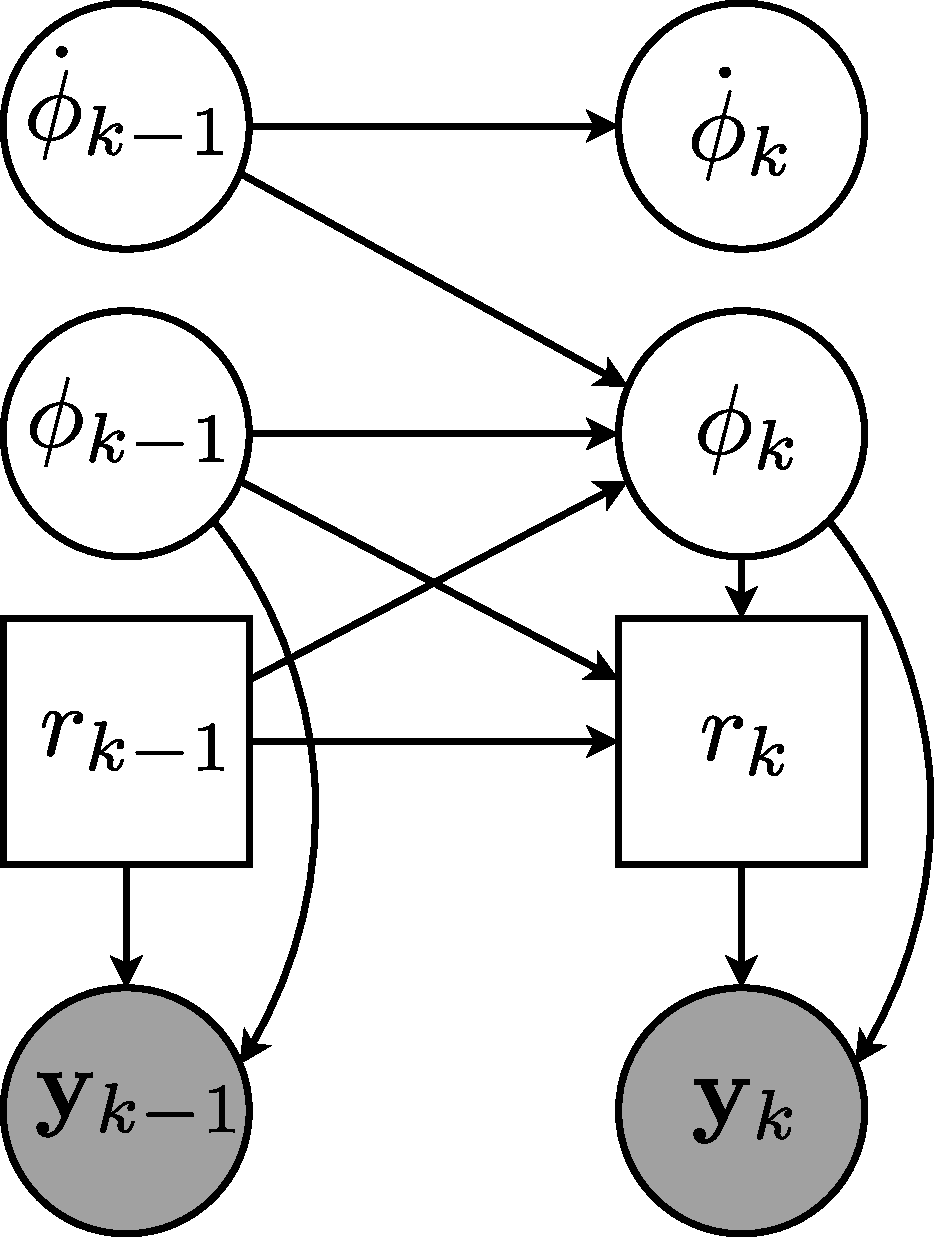
\includegraphics[scale=0.27]{models/model_bpm.pdf}
    } \hspace{1cm}
    \subfloat[Bar pointer model using a mixture observation model (\momodel)]{\label{fig:dbn:bpmmix}
      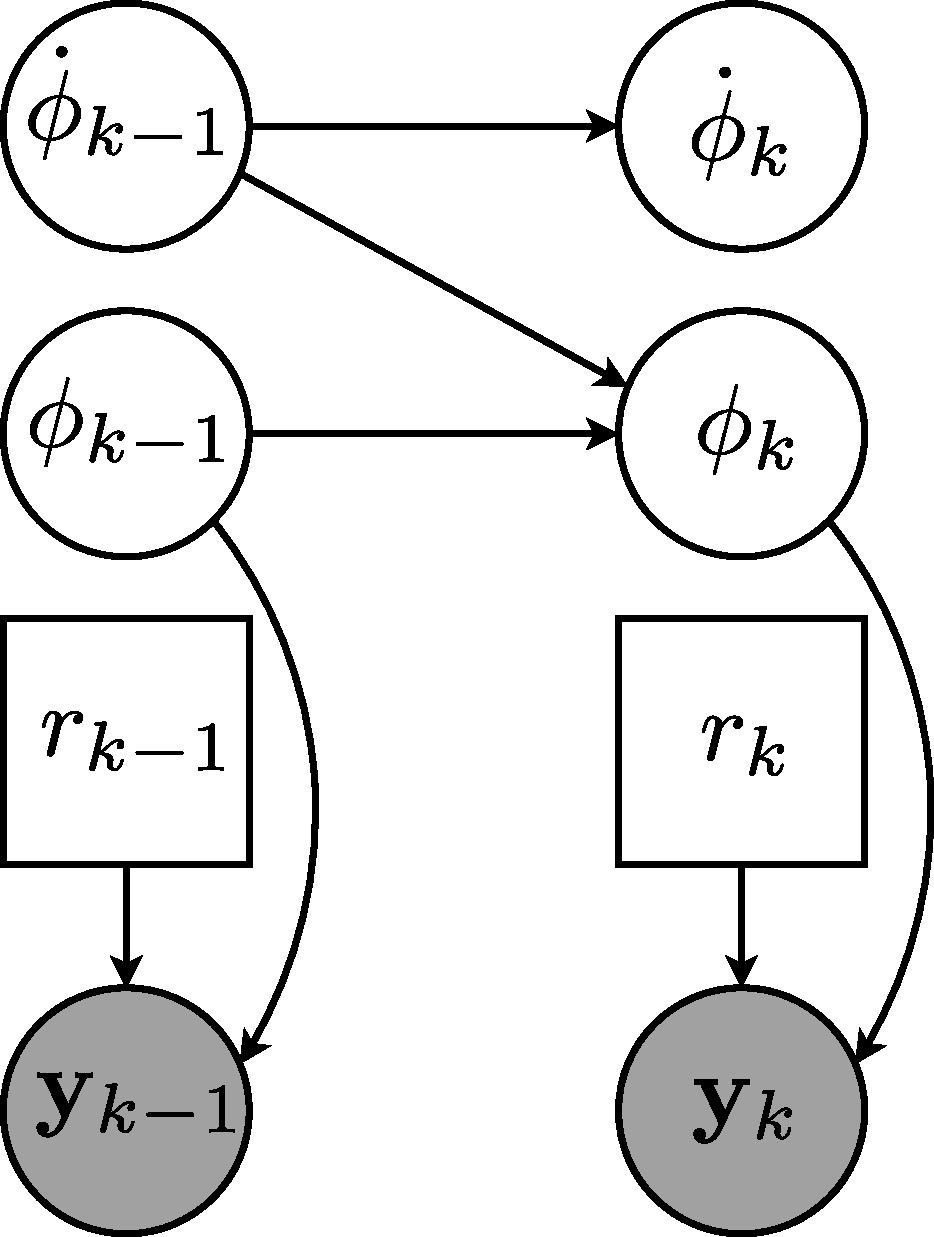
\includegraphics[scale=0.27]{models/model_mix.pdf}
    }\\
		\subfloat[Section pointer model (\spmodel)]{\label{fig:dbn:spm}
      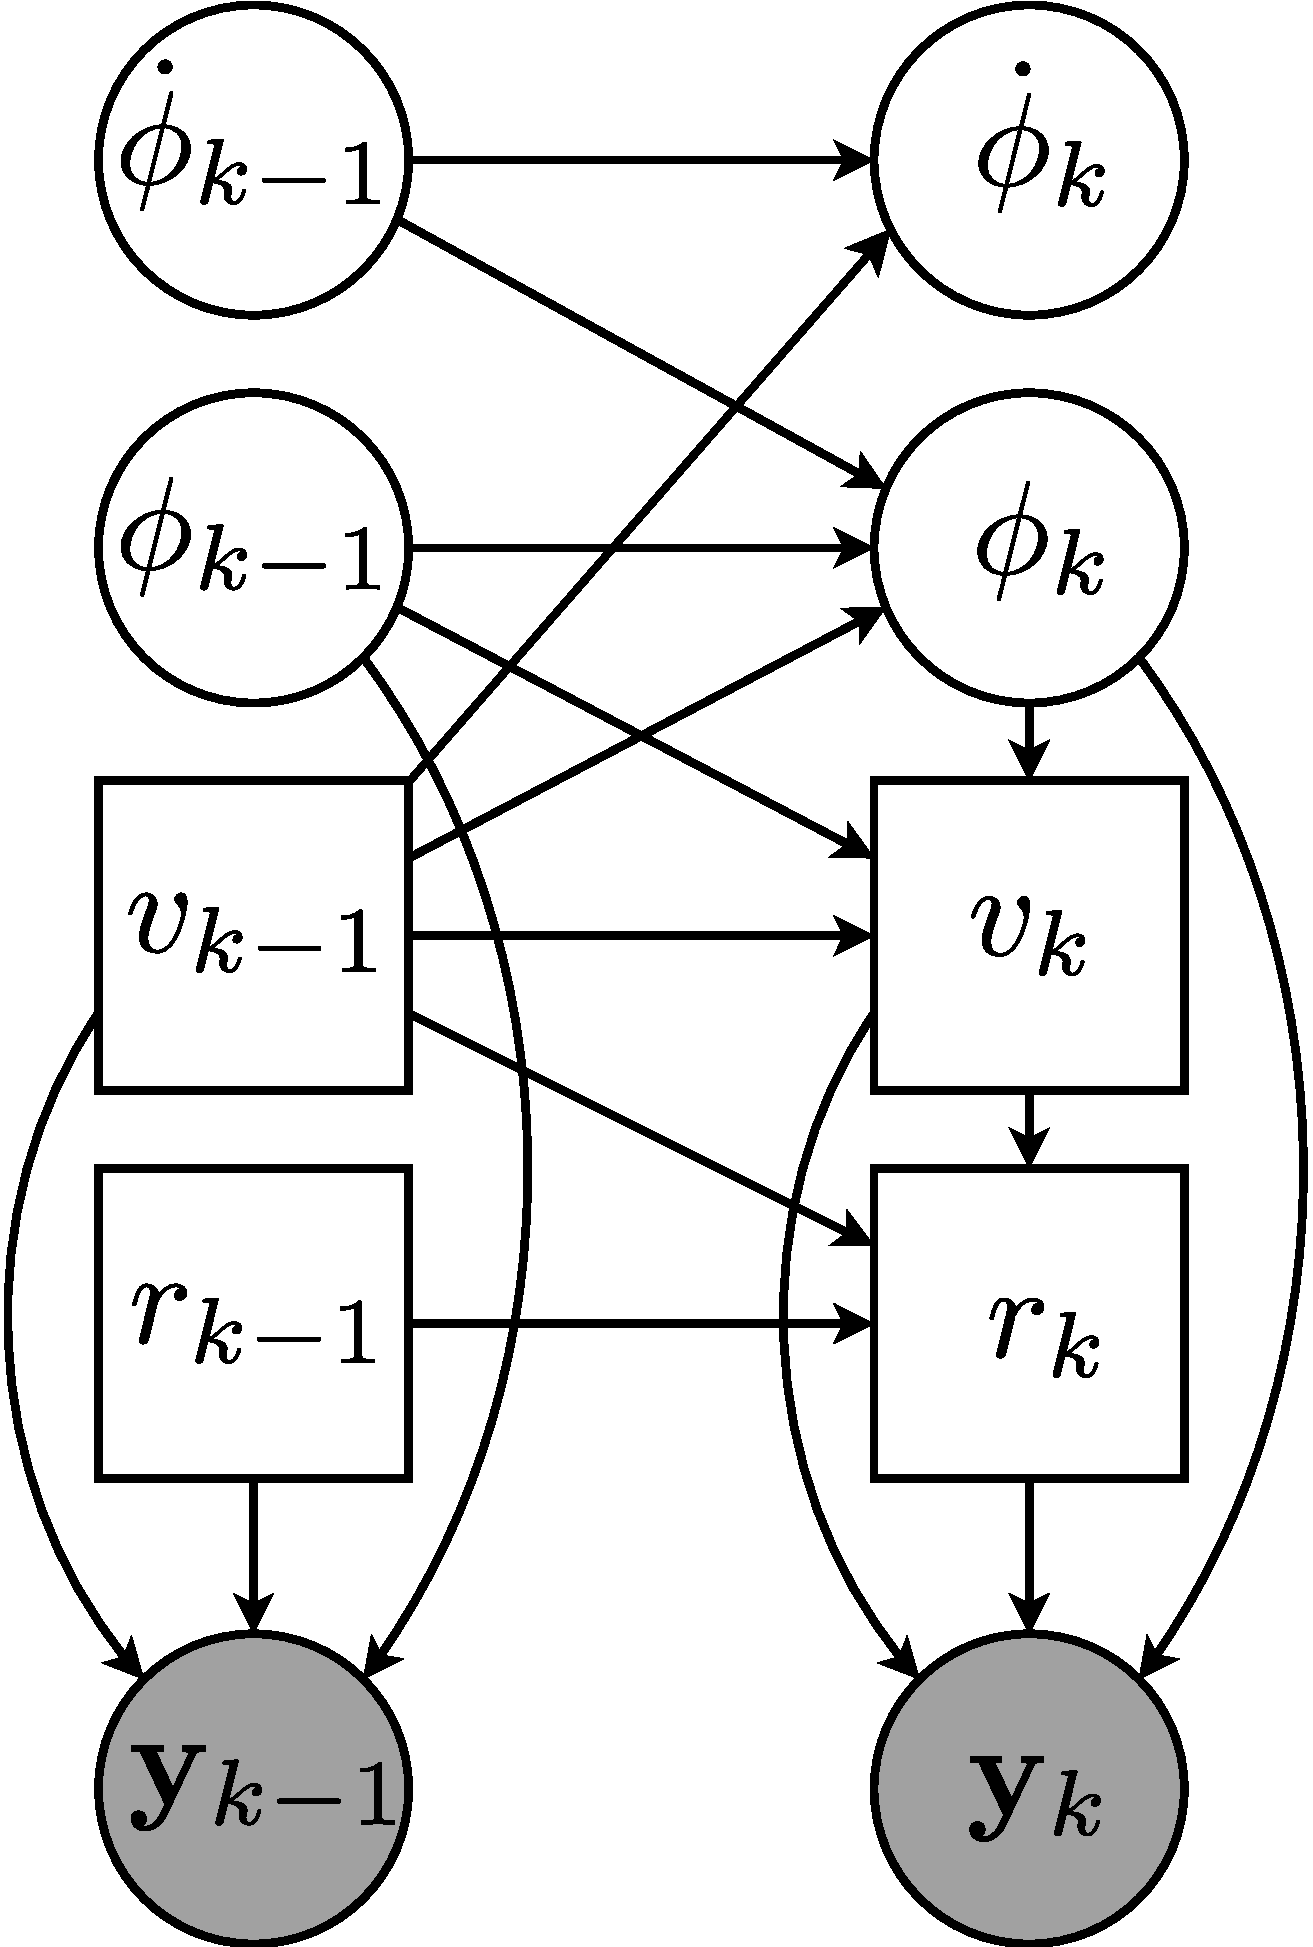
\includegraphics[scale=0.21]{models/model_spm_new.pdf}
    } \hspace{0.5cm}
    \subfloat[Simplified section pointer model]{\label{fig:dbn:spmOnePatt}
      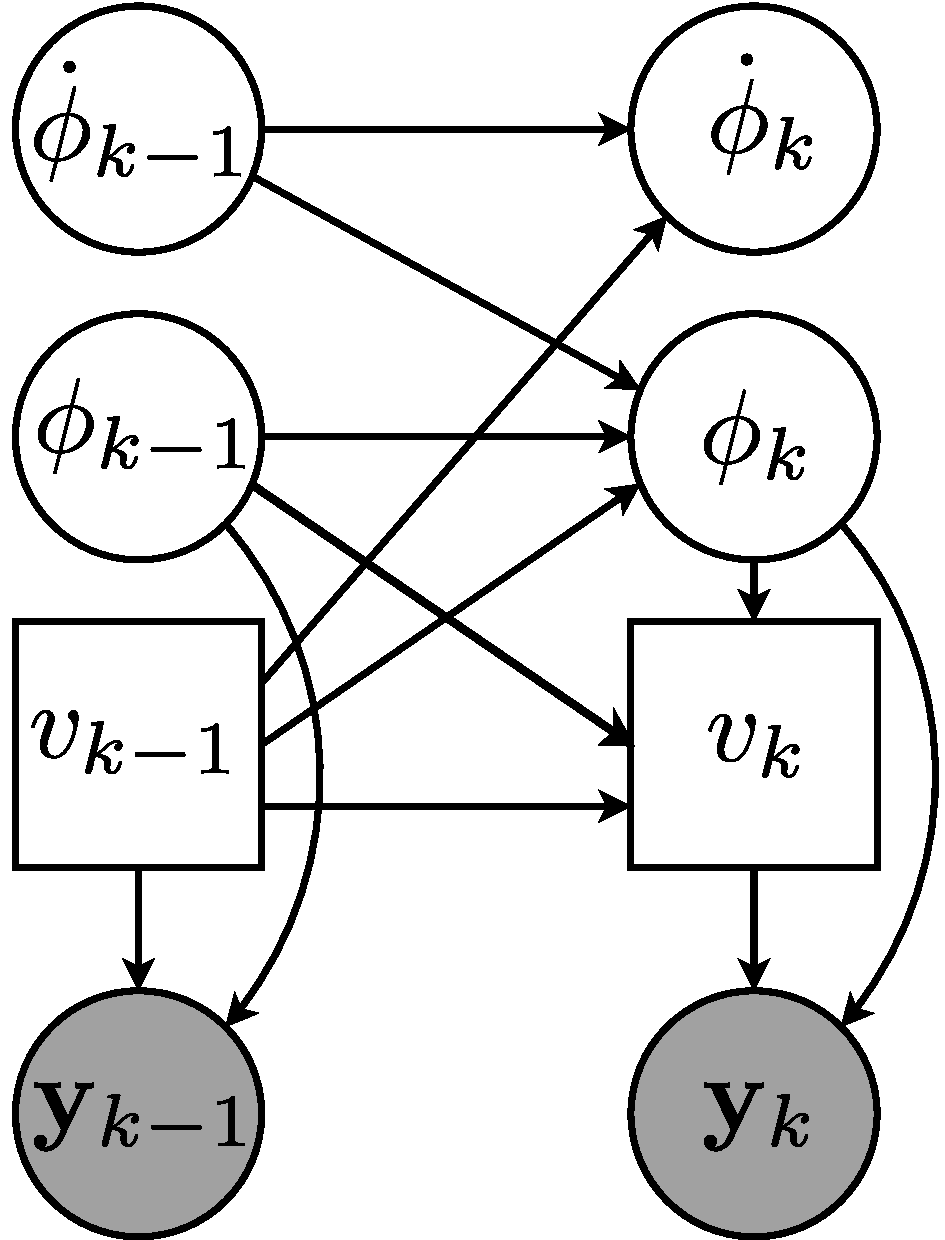
\includegraphics[scale=0.27]{models/model_spm_icassp16.pdf}
    } 
\caption[The meter analysis models used in the dissertation]{The meter analysis models used in the dissertation. In each of these \glspl{DBN}, circles and squares denote continuous and discrete variables, respectively. Grey nodes and white nodes represent observed and latent variables, respectively.}\label{fig:dbn:all}
\end{figure}
%
The bar pointer model\index{Bar pointer model} (or dynamic bar pointer model), referred to as \bpmodel\ in this chapter, is a generative model that has been successfully applied for meter analysis tasks. The model assumes a hypothetical time pointer within a bar that progresses at the speed of the tempo to traverse through the bar and then reinitializes at the end of the bar to track the next bar. The model also assumes that specific bar length rhythm patterns\index{Rhythm pattern} are played in a bar depending on the rhythmic style, and uses these patterns to track the progression through the bar. These rhythmic patterns can be fixed \textit{a priori} or learned from data to build an observation model for each position in the bar. When learned from data, the rhythmic patterns are built using a signal representation derived from audio, most often from frame level audio features to preserve the temporal information in features. Progressing through the bar, the model can hence be used to sample the observation model and generate a rhythmic pattern that is possible and allowed in the rhythm style. The model allows for different metrical structures, tempi ranges and rhythm styles, providing a flexible framework for meter analysis. Though applied only for meter analysis from audio recordings in this dissertation, the \bpmodel\ can be applied even to symbolic music~\cite{whiteley:06:ismir}. \bpmodel\ can be represented as a \gls{DBN} with specific conditional dependence relations between the variables that lead to several variants and extensions of the model. The structure of the \bpmodel\ is shown in \figref{fig:dbn:bpm}.

In a \gls{DBN}, an observed sequence of features derived from an audio signal $\obsVar_{1:\nframes} = \{\obsVar_1, \ldots, \obsVar_\nframes\}$ is generated by a sequence of hidden (latent) variables $\hidVar_{1:\nframes} \!=\! \{\hidVar_1, \ldots, \hidVar_\nframes\}$, where $\nframes$ is the length of the feature sequence (number of audio frames in an audio excerpt). The joint probability distribution of hidden and observed variables factorizes as, 
\begin{equation}
P(\obsVar_{1:\nframes},\hidVar_{0:\nframes}) = P(\hidVar_{0}) \cdot \overset{\nframes}{\underset{k=1}{\prod}}  P(\hidVar_{k} \mid \hidVar_{k-1})\,P(\obsVar_{k} \mid \hidVar_{k}) \label{eqn:dbn:basic}
\end{equation}
where, $P(\hidVar_{0})$ is the initial state distribution, $P(\hidVar_{k} | \hidVar_{k-1})$ is the transition model, and $P(\obsVar_{k} | \hidVar_{k})$ is the observation model.
%
\subsubsection{Hidden variables}
\begin{figure}[t]
\centering
	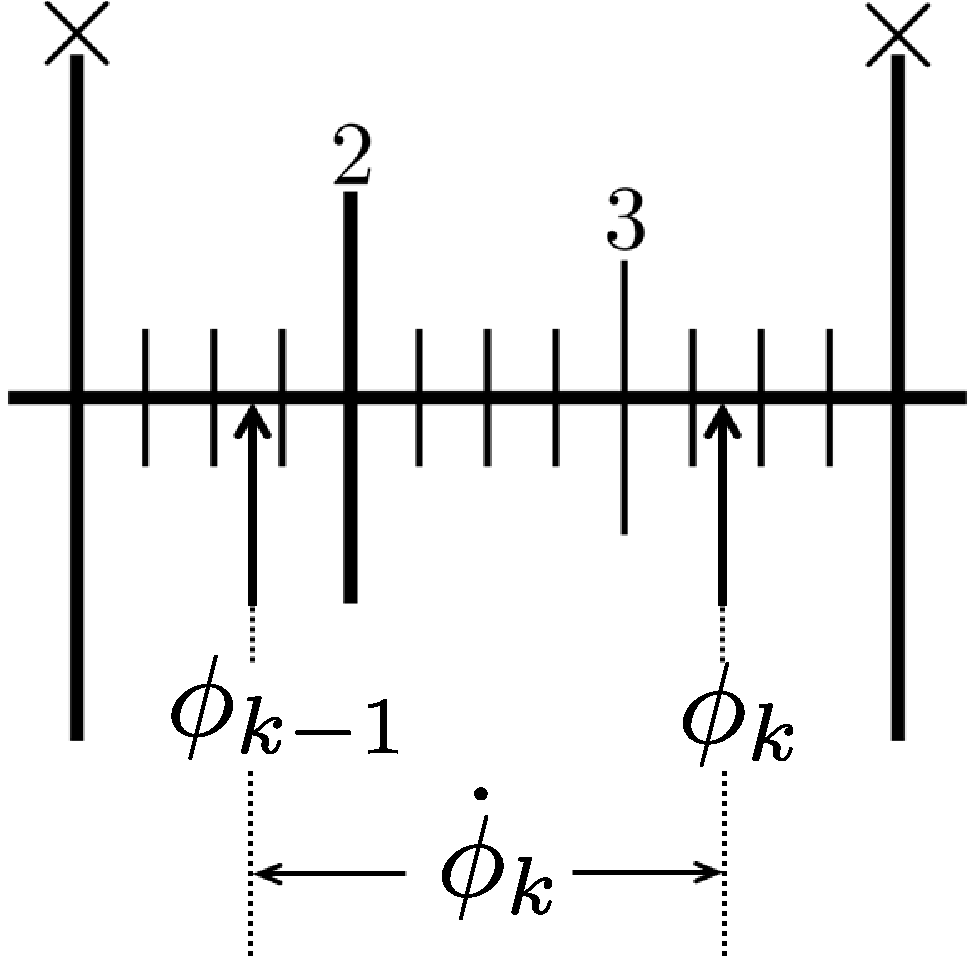
\includegraphics[scale=0.25]{meterTrack/bpm-illustration.pdf}
	\caption[An illustration of the bar pointer model]{An illustration of the progression of bar position and instantaneous tempo variables over two consecutive audio frames in a cycle of \gls{rupaka} \gls{tala}. The effect of instantaneous tempo is greatly exaggerated for clarity in the illustration.}
	\label{fig:bpm:illustration}
\end{figure}
%
In the bar pointer model, at each audio frame $k$, the hidden variable vector $\hidVar_{k}$ describes the state of a hypothetical bar pointer $\hidVar_{k} = [\mpos_k \; \tempoVar_k \; \rpattVar_k]$, representing the bar position, instantaneous tempo and a rhythmic pattern indicator, respectively (see \figref{fig:bpm:illustration} for an illustration).
%
\begin{itemize}[leftmargin=*]
\item \textit{Rhythmic pattern indicator}: The rhythmic pattern variable $\rpattVar \in \lbrace 1, \ldots, \nrhythmPatts\rbrace$ is an indicator variable to select one of the $\nrhythmPatts$ observation models corresponding to each bar (cycle) length rhythmic pattern of a rhythm class. Each pattern $\rpattVar$ has an associated length of cycle $\npos_\rpattVar$ and number of beat (or \gls{matra}) pulses $\nbeats_\rpattVar$. In the scope of this dissertation, all rhythmic patterns are learned from training data and not fixed \textit{a priori}. We can infer the rhythm class or meter type (\gls{tala}) by allowing rhythmic patterns of different lengths from different rhythm classes to be present in the model, as used by \citeA{krebs:15:pf}. However, it is to be noted that for the problem of meter tracking, we assume that the cycle length is known and that all the $\nrhythmPatts$ rhythmic patterns belong to the same rhythm class (\gls{tala}), $\npos_\rpattVar = \npos$ and $\nbeats_\rpattVar = \nbeats$~$\forall \, \rpattVar$. 

\item \textit{Bar position}: The bar position $\mpos \in [0, \npos_\rpattVar)$ variable indicates a position in the bar at any audio frame and tracks the progression through the bar. Here, $\npos_\rpattVar$ is the length of the bar (cycle), which is also the length of the bar length rhythmic pattern being tracked. The bar position variable traverses the whole bar and wraps around to zero at the end of the bar to track the next bar. The maximum value of bar (cycle) length, $\npos$, depends on the longest bar (cycle) that is tracked. We set the length of the longest bar being tracked to a fixed value, and scale other bar (cycle) lengths accordingly. 
\item \textit{Instantaneous tempo}: Instantaneous tempo $\tempoVar$ is the rate at which the bar position variable progresses through the cycle at each time frame, measured in bar positions per time frame. The range of the variable $\tempoVar_k \in [\tempoVar_{\min}, \tempoVar_{\max}]$ depends on the length of the cycle $\npos$ and the analysis frame hop size ($\framehop = $ 0.02 second used in this thesis), and can be preset or learned from data. A tempo value of $\tempoVar_{k}$ corresponds to a bar (cycle) length of ($\framehop \cdot \npos_\rpattVar / \tempoVar_{k}$) seconds and ($60 \cdot \nicefrac{\nbeats\cdot\tempoVar_k}{(\npos \cdot\framehop)})$ beats/\glspl{matra} per minute. The range of the variable can be used to restrict the range of tempi that is allowed within each rhythm class. 
\end{itemize}
\subsubsection{Initial state distribution}
The initial state distribution $P(\hidVar_{0})$ can be used to incorporate prior information about the metrical structure of the music into the model. Different initializations are explored depending on the meter analysis task under consideration. A uniform initialization is used for meter inference and tracking, while a narrower informed initialization is done for informed meter tracking. 
\subsubsection{Transition model}
Given the conditional dependence relations between the variables of the \bpmodel\ in \figref{fig:dbn:bpm}, the transition model factorizes as, 
\begin{multline}\label{eqn:bpm:transx}
P(\hidVar_{k} \mid \hidVar_{k-1})=P(\mpos_{k} \mid \mpos_{k-1},\tempoVar_{k-1},\rpattVar_{k-1})P(\tempoVar_{k} \mid \tempoVar_{k-1}) \\ P(\rpattVar_{k} \mid \rpattVar_{k-1},\mpos_{k},\mpos_{k-1})
\end{multline}
The individual terms of the equation can be expanded as, 
\begin{equation}\label{eqn:bpm:transmpos}
P(\mpos_{k} \mid \mpos_{k-1},\tempoVar_{k-1},r_{k-1})=\indicator_{\mpos}
\end{equation}
where $\indicator_{\mpos}$ is an indicator function that takes a value of one if $\mpos_{k} = (\mpos_{k-1} + \tempoVar_{k-1})\!\!\!\mod\!\!(\npos_{\rpattVar_{k-1}})$ and zero otherwise. The tempo transition is given by,
\begin{equation}\label{eqn:bpm:transtempo}
P(\tempoVar_{k} \mid \tempoVar_{k-1})\propto\mathcal{N}(\tempoVar_{k-1},\sigma_{\tempoVar_k}^{2})\times \indicator_{\tempoVar}
\end{equation}
where $\indicator_{\tempoVar}$ is an indicator function that equals one if $\tempoVar_{k} \in [\tempoVar_{\textrm{min}}, \tempoVar_{\textrm{max}}]$ and zero otherwise, restricting the tempo to be between a predefined range. $\normDist(\mu,\sigma^2)$ denotes a normal distribution with mean $\mu$ and variance $\sigma^{2}$. The value of $\sigma_{\tempoVar_{k}}$ depends on the value of tempo to allow for larger tempo variations at higher tempi. % and the length of the pattern, \cdot (\nicefrac{\npos_{\rpattVar_{k-1}}}{\npos})
We set $\sigma_{\tempoVar_k} = \sigma_n \cdot \tempoVar_{k-1}$, where $\sigma_n$ is a user parameter that controls the amount of local tempo variations we allow in the music piece. The pattern transitions are governed by, 
\begin{equation}\label{eqn:bpm:transpatt}
P(\rpattVar_{k} \mid \rpattVar_{k-1},\mpos_{k},\mpos_{k-1}) = 
\begin{cases}
 \tmPatt(\rpattVar_{k-1},\rpattVar_{k}) & \text{if} \,\,\, \mpos_{k} < \mpos_{k-1}\\
\indicator_{\rpattVar} & \text{else}
\end{cases}
\end{equation}
where, $\tmPatt$ is the $\nrhythmPatts \times \nrhythmPatts$ time-homogeneous transition matrix with $\tmPatt(i, j)$ being the transition probability from $\rpattVar_i$ to $\rpattVar_j$, and $\indicator_{r}$ is an indicator function that equals one when $\rpattVar_k = \rpattVar_{k-1}$ and zero otherwise. Since the rhythmic patterns are one bar (cycle) in length, pattern transitions are allowed only at the end of the bar (cycle). When there are multiple patterns, these transition probabilities indicate the most probable movement through these patterns from bar to bar, as the piece progresses. To reflect the performance practice, the pattern transition probabilities are learned from data.
\subsubsection{Observation model}
The observation model aims to model the underlying rhythmic patterns present in the metrical structure being inferred/tracked, explaining the possible rhythmic events at each position in the bar. Some of the positions in a bar have a higher probability of an onset occurring than other parts (e.g. the positions corresponding to downbeats, beats). Further, the strength of these onsets also vary depending on accent patterns of a rhythm class (which can be modeled from labeled data). The observation model used in this dissertation aims to address both these aspects (the locations and strengths of the rhythmic events), and closely follows the observation model proposed by \citeA{krebs:13:bpm}. 

The utility of spectral flux based rhythmic audio features was outlined in preliminary experiments \secref{sec:mt:earlyexpts}. A similar audio derived spectral flux\index{Spectral flux} feature is used in this dissertation as well, identical to features used by \citeA{krebs:13:bpm}, as explained in \secref{sec:cmrdataset} (see \figref{fig:obs:featcomp}). Since the bass onsets have significant information about the rhythmic patterns, the features are computed in two frequency bands (Low: $\leq$ 250 Hz, High: $>$ 250 Hz). 

It is assumed that the audio features depend only on the bar position and rhythmic pattern variables, without any influence from tempo. While this assumption is not completely true, it simplifies the observation model and helps to train better models with limited training data. Further, it is assumed that the audio features do not vary too much over short changes in position in cycle (e.g. the spectral flux variations within a small fraction of an \gls{akshara} might be negligible), which additionally helps to tie several positions to have the same observation probability and helps train models with limited training data.

Using beat and downbeat annotated training data, the audio features are then grouped into bar length patterns. The bar is then discretized into 64$^{\mathrm{th}}$ note cells (four cells per \gls{akshara} for Carnatic music, and four cells per \gls{matra} for Hindustani music, corresponds to $25$ bar positions with $\npos = 1600$). A k-means clustering algorithm clusters and assigns each bar of the dataset to one of the $\nrhythmPatts$ rhythmic patterns. All the features within the cell are then collected for each pattern, and maximum likelihood estimates of the parameters of a two component \gls{GMM} are obtained. The observation probability within a 64$^{\mathrm{th}}$ note cell is assumed to be constant, and computed as, 
\begin{equation}\label{eqn:bpm:obsmodel}
P(\obsVar \mid \hidVar) = P(\obsVar \mid \mpos,\rpattVar) = \overset{2}{\underset{i=1}{\sum}}\pi_{\mpos,\rpattVar,i}\,\normDist(\obsVar;\boldsymbol{\mu}_{\mpos,\rpattVar,i},\boldsymbol{\Sigma}_{\mpos,\rpattVar,i})
\end{equation}
where, $\normDist(\obsVar;\boldsymbol{\mu},\boldsymbol{\Sigma})$ denotes a normal distribution of the two dimensional feature $\obsVar$. For the mixture component $i$, $\pi_{\mpos,\rpattVar,i}, \boldsymbol{\mu}_{\mpos,\rpattVar,i}$ and $\boldsymbol{\Sigma}_{\mpos,\rpattVar,i}$ are the component weight, mean (2-dimensional) and the covariance matrix ($2\times2$), respectively.
% 
\subsubsection{Inference in bar pointer model}
The goal of inference in meter analysis tasks is to find a hidden variable sequence that maximizes the posterior probability of the hidden states given an observed sequence of features: a \gls{MAP} sequence $\hidVar^{\optstar}_{1:\nframes}$ that maximizes $P(\hidVar_{1:\nframes} \mid \obsVar_{1:\nframes})$. The inferred hidden variable sequence $\hidVar^{\optstar}_{1:\nframes}$ can then be translated into a sequence of: 
\begin{itemize}[noitemsep]
	\item downbeat (\gls{sama}) instants: $\samaSet = \{\timeVar^{\optstar}_k \mid \mpos^{\optstar}_k = 0\}$
	\item beat instants: $\beatSet = \{\timeVar^{\optstar}_k \mid \mpos^{\optstar}_k = i \cdot \nicefrac{\npos_{\rpattVar^\optstar}}{\nbeats_{\rpattVar^\optstar}}$, $i = 1,\ldots,\nbeats_\rpattVar \}$
	\item local instantaneous tempo: $\tempoVar^{\optstar}_k$
	\item estimated rhythmic patterns: $\rpattVar^{\optstar}$
\end{itemize}
Two different inference schemes are now described, an inference using the Viterbi algorithm in a discretized state space, and an approximate inference using particle filters in the continuous space of $\mpos$ and $\tempoVar$, with the discrete variable $\rpattVar$. 
\subsubsection{Viterbi algorithm}
The continuous variables of bar position and tempo can be discretized, which transforms the \gls{DBN} into an \gls{HMM} over the cartesian product space of the discretized variables. In the \gls{HMM}, an inference can be performed using the Viterbi algorithm to compute the most likely sequence of hidden states given the observed feature sequence.  
% We follow the discretization that closely follows the method proposed by \citeA{krebs:15:pf}, by replacing the continuous variables $\mpos$ and $\tempoVar$ by their discretized counterparts, 
% \small
% \begin{eqnarray}
% 	m\!\!&\in&\!\!\{1,2,\ldots,\lceil \npos_\rpattVar \rceil\} \label{eqn:bpm:discmpos}\\
% 	n\!\!&\in&\!\!\{\tempoVar_{\min}, \tempoVar_{\min}\!+\!\deltatempo, \tempoVar_{\min}\!+\!2\deltatempo, \cdots, \tempoVar_{\max}\!-\!\deltatempo, \tempoVar_{\max}\} \label{eqn:bpm:disctempo}
% \end{eqnarray}
% \normalsize
% where $\deltatempo$ is the resolution of the tempo grid, and is computed as $\deltatempo = \nicefrac{(\tempoVar_{\max} - \tempoVar_{\min})}{(\ntempo-1)}$, where $\ntempo$ denotes the number of discrete tempo states. 
% 
% With such a discretization in place, the transition model equations \eqnref{eqn:bpm:transx}, \eqnref{eqn:bpm:transmpos} and \eqnref{eqn:bpm:transpatt} remain as defined. However, the tempo transition probability is redefined within the allowed tempo range as, 
% \begin{equation}
% P(n_{k} \mid n_{k-1}) = 
% \begin{cases}
% 1-p_{n} & \text{if} \,\,\, n_{k}=n_{k-1} \\
% \frac{p_n}{2} & \text{if} \,\,\, n_{k}=n_{k-1} \pm \deltatempo \\
% 0 & \text{otherwise}
% \end{cases}
% \end{equation}

We follow a discretization scheme that is identical to the method proposed by \citeA{krebs:15:pf}, by replacing the continuous variables $\mpos$ and $\tempoVar$ by their discretized counterparts $\mposDisc$ and $\tempoVarDisc$, respectively, as 
\begin{eqnarray}
	\mposDisc & \in & \{1,2,\ldots,\lceil \npos_\rpattVar \rceil\} \label{eqn:bpm:discmpos}\\
	\tempoVarDisc & \in & \{\tempoVarDisc_{\min}, \tempoVarDisc_{\min} + 1, \tempoVarDisc_{\min} + 2, \cdots, \ntempo - 1, \ntempo\} \label{eqn:bpm:disctempo}
\end{eqnarray}
Here, $\tempoVarDisc_{\min} = \lfloor \tempoVar_{\min} \rfloor$ and $\ntempo = \tempoVarDisc_{\max} = \lceil \tempoVar_{\max} \rceil$ is the discrete minimum and maximum tempo values allowed, where $\lfloor \cdot \rfloor$ and $\lceil \cdot \rceil$ denote floor and ceil operations, repsectively. 

With such a discretization in place, the transition model equations \eqnref{eqn:bpm:transx}, \eqnref{eqn:bpm:transmpos} and \eqnref{eqn:bpm:transpatt} remain as defined. However, the tempo transition probability is redefined within the allowed tempo range as, 
\begin{equation} \label{eqn:bpm:hmmntrans}
P(\tempoVarDisc_{k} \mid \tempoVarDisc_{k-1}) = 
\begin{cases}
1-p_{n} & \text{if} \,\,\, \tempoVarDisc_{k}=\tempoVarDisc_{k-1} \\
\frac{p_n}{2} & \text{if} \,\,\, \tempoVarDisc_{k}=\tempoVarDisc_{k-1} \pm 1 \\
0 & \text{otherwise}
\end{cases}
\end{equation}
where $p_n$ is the probability of tempo change. It is to be noted that that the discretization of $\mpos$ and $\tempoVar$ need not be done on an integer or on a uniform grid. It is possible that the tempo range can be non-uniformly sampled, as was proposed by \citeA{krebs:15:ismir}. In this dissertation, however, only a uniform discretization is explored in the context of the \gls{HMM}. Viterbi algorithm~\cite{rabiner:89:tutorial}\index{Viterbi decoding} is then used to obtain a \gls{MAP} sequence of states with the \gls{HMM}. The \gls{HMM} based Viterbi decoding inference algorithm in \bpmodel\ as described in the section will be denoted as \acrshort{hmmprior} in the dissertation. 

The drawback of this approach is that the discretization has to be on a very fine grid in order to guarantee good performance, which leads to a prohibitively large state space (specially with long cycles) and, as a consequence, to a computationally demanding inference. The size of the state space is $\mathfrak{S} = \npos \cdot \ntempo \cdot \nrhythmPatts$ and needs a $\mathfrak{S}\times\mathfrak{S}$ sized transition matrix. As an example, dividing a bar into $\npos = 1600$ position states, with $\ntempo = 15$ tempo states and $\nrhythmPatts = 4$ patterns, the size of the state space is $\mathfrak{S} = 96000$ states. The computational complexity of the Viterbi algorithm is $\bigO(\nframes\!\cdot\!\lvert \mathfrak{S} \rvert ^2)$. Even though the state transition matrix is sparse due to a lower number of allowed transitions leading to a complexity of $O(\nframes \cdot \npos \cdot \nrhythmPatts)$, the inference with \gls{HMM} can become computationally prohibitive and does not scale well with increasing number of states. This problem can be overcome, for instance, by using approximate inference methods such as particle filters. 
\subsubsection{Particle Filter (PF)}
Particle filters\index{Particle filter} (or \gls{SMC} methods) are a class of approximate inference algorithms to estimate the posterior density in a state space. They overcome two main problems of the \gls{HMM} - discretization of the state space and the quadratic scaling up of the size of state space with additional hidden variables. In addition, they can incorporate long term relationships between hidden variables. 

In the continuous state space of $\hidVar_{1:\nframes}$, the exact computation of the posterior $P(\hidVar_{1:\nframes}|\obsVar_{1:\nframes})$ is often intractable, but it can be evaluated pointwise. In particle filters, the posterior is approximated using a weighted set of points (known as particles) in the state space as,
\begin{equation}\label{eqn:bpm:pfposterior}
P(\hidVar_{1:\nframes} \mid \obsVar_{1:\nframes})\approx\overset{\nparticles}{\underset{i=1}{\sum}}w_{\nframes}^{(i)}\delta(\hidVar_{1:\nframes}-\hidVar_{1:\nframes}^{(i)})
\end{equation}
Here, $\{\hidVar^{(i)}_{1:\nframes}\}$ is a set of points (particles) with associated weights $\{\weight_{\nframes}^{(i)}\}$, $i = 1,\ldots,N_p$, $\hidVar_{1:\nframes}$ is the set of all state trajectories until frame $\nframes$, $\delta(x)$ is the Dirac delta function, and $\nparticles$ is the number of particles. 

With this particle system, starting with $P(\hidVar_0)$, to approximate the posterior pointwise, we need a suitable method to draw samples $\hidVar^{(i)}_k$ and compute appropriate weights $\weight_{k}^{(i)}$ recursively at each time step. It is clearly non-trivial to sample from an arbitrary posterior distribution. A simple approach is \gls{SIS}~\cite{doucet:09:tutorial}, where we sample from a \textsl{proposal} distribution $Q(\hidVar_{1:k} | \obsVar_{1:k})$ that has the same support and is as similar to the true (target) distribution $P(\hidVar_{1:k} | \obsVar_{1:k})$ as possible. To account for the fact that we sampled from a proposal and not the target, we attach an importance weight $\weight^{(i)}_k$ to each particle, computed as, 
\begin{equation}\label{eqn:bpminf:proposal}
\weight^{(i)}_{k} = \frac{P(\hidVar_{1:k} \mid \obsVar_{1:k})}{Q(\hidVar_{1:k} \mid \obsVar_{1:k})}
\end{equation}
With a suitable proposal density, these weights can be computed recursively as, 
\begin{equation}\label{eqn:bpminf:wtupdate}
\weight_{k}^{(i)}\propto \weight_{k-1}^{(i)}\frac{P(\obsVar_{k} \mid \hidVar_{k}^{(i)})P(\hidVar_{k}^{(i)} \mid \hidVar_{k-1}^{(i)})}{Q(\hidVar_{k}^{(i)} \mid \hidVar_{k-1}^{(i)},\obsVar_{k})}
\end{equation}
Following \citeA{krebs:15:pf}, we choose to sample from the transition probability $Q(\hidVar_{k}^{(i)} \mid \hidVar_{k-1}^{(i)},\obsVar_{k}) = P(\hidVar_{k}^{(i)} \mid \hidVar_{k-1}^{(i)})$, which reduces \eqnref{eqn:bpminf:wtupdate} to 
\begin{equation}\label{eqn:bpminf:wtSIS}
\weight_{k}^{(i)}\propto w_{k-1}^{(i)}P(\obsVar_{k} \mid \hidVar_{k}^{(i)})
\end{equation}
The \gls{SIS} algorithm derives samples by first sampling from proposal, in this case the transition probability and then computes weights according to \eqnref{eqn:bpminf:wtSIS}. Once we determine the particle trajectories $\{\hidVar^{(i)}_{1:\nframes}\}$, we then select the trajectory $\hidVar^{(i^{*})}_{1:\nframes}$ with the highest weight $\weight^{(i^{*})}_K$ as the \gls{MAP} state sequence. 

Many extensions have been proposed to the basic \gls{SIS} filter (\citeA{doucet:09:tutorial} provide a comprehensive overview) to address several problems with it. Some of the relevant extensions are briefly mentioned, emphasizing their key aspects. A more detailed description of the algorithms has been presented by \citeA{krebs:15:pf}. 

The most challenging problem in particle filtering is the degeneracy problem, where within a short time, most of the particles have a weight close to zero, representing unlikely regions of state space. This is contrary to the ideal case when we want the proposal to match well with the target distribution leading to a uniform weight distribution with low variance. To reduce the variance of the particle weights, resampling steps are necessary, which replace low weight particles with higher weight particles by selecting particles with a probability proportional to their weights. Several resampling methods have been proposed, but we use systematic resampling in this dissertation as recommended by \citeA{doucet:09:tutorial}. With resampling as the essential difference, the \gls{SIS} filter with resampling is called as \gls{SISR} filter. 

In meter analysis problems, due to metrical ambiguities, the posterior distribution $P(\hidVar_k | \obsVar_{1:k})$ is highly multimodal. Resampling tends to lead to a concentration of particles in one mode of the posterior, while the remaining modes are not covered. One way to alleviate this problem is to compress the weights $\weightVec_k = \{\weight^{(i)}_k\}$, $i = 1,\ldots, \nparticles$ by a monotonically increasing function to increase the weights of particles in low probability regions so that they can survive resampling. After resampling, the weights have to be uncompressed to give a valid probability distribution. This can be formulated as an \gls{APF} \cite{johansen:08:auxpf}.

A particle system that is capable of handling metrical ambiguities must maintain the multimodality of posterior distribution and be able to track several hypotheses together, which \gls{SISR} and \gls{APF} cannot do explicitly. A system called the \gls{MPF} was proposed by \citeA{vermaak:03:multimodal} to track multiple hypotheses, and was adapted to meter inference by \citeA{krebs:15:pf}. 

In a \gls{MPF}, each particle is assigned to a cluster that (ideally) represents a mode of the posterior. During resampling, the particles of a cluster interact only with particles of the same cluster. Resampling is done independently in each cluster, while maintaining the probability distribution intact. This way, all the modes of the posterior can be tracked through the whole audio piece, and the best hypothesis can be chosen at the end. In this work, we use an identical clustering scheme using a cyclic distance measure as described by \citeA{krebs:15:pf} to track several different possible metrical positions at a given time. We use a cyclic distance measure that can take into account the cyclic nature of the bar position $\mpos$. By representing the bar position as a complex phasor on the unit circle, we can compute the corresponding angle $\varphi(\mpos_k) = \nicefrac{2\pi \mpos_k}{\npos}$. A distance between two particles indexed by $i$ and $j$ can then be computed as, 
\begin{multline}
d(i,j)=\lambda_{\mpos}\left[\left(\cos(\varphi^{(i)})-\cos(\varphi^{(j)})\right)^{2}\!+\!\left(\sin(\varphi^{(i)})-\sin(\varphi^{(j)})\right)^{2}\right]\\
+\lambda_{\tempoVar}\left(\tempoVar^{(i)}-\tempoVar^{(j)}\right)^{2}+\lambda_{\rpattVar}(\rpattVar^{(i)}-\rpattVar^{(j)})^{2}
\end{multline}
where, the parameters $[\lambda_{\mpos}$, $\lambda_{\tempoVar}$, $\lambda_{\rpattVar}]$ control the relative weights in the distance. 

In the \gls{MPF}, after an initial cluster assignment, we perform a reclustering before every resampling step, merging or splitting clusters based on the average distance between cluster centroids. The clustering, merging and splitting of clusters is necessary to control the number of clusters, which ideally represents the number of modes in the posterior. The mixture particle filter can be combined with auxiliary resampling to give the \gls{AMPF}. As recommended by \citeA{krebs:15:pf}, we resample at a fixed interval $\sampInterval$. 
%
\begin{algorithm}
\caption{An outline of the \acrshort{pfprior} algorithm (\gls{AMPF} for inference in \bpmodel)}\label{algo:pf:prior}
  \begin{algorithmic}[1]
      \For{i = 1 to \nparticles} 
         \State Sample $\hidVar^{(i)}_0 \sim P(\hidVar_0)$  \Comment{$\hidVar_k = [\mpos_k,\tempoVar_k,\rpattVar_k]$}
         \State Set $\weight_{0}^{(i)} = \nicefrac{1}{\nparticles}$
      \EndFor
      \State Cluster $\{\hidVar^{(i)}_0 | i = 1, 2, \cdots, \nparticles\}$, get cluster assignments $\{\clust^{(i)}_0\}$
      % Main iteration
      \For{k = 1 to \nframes}
         \For{i = 1 to \nparticles} \Comment{\mpos, \rpattVar: Proposal and weights}
            \State Sample $\mpos^{(i)}_{k} \sim P(\mpos^{(i)}_{k} \mid \hidVar^{(i)}_{k-1})$, Set $\clust^{(i)}_k = \clust^{(i)}_{k-1}$
            \If{$\mpos^{(i)}_{k} < \mpos^{(i)}_{k-1}$}    \Comment{Bar crossed}
               \State $\rpattVar_k^{(i)} \sim P(\rpattVar_k^{(i)} \mid \rpattVar_{k-1}^{(i)})$ \Comment{Sample patterns}
            \Else
               \State $\rpattVar_k^{(i)} = \rpattVar_{k-1}^{(i)}$
            \EndIf
            \State $\tilde{\weight}_{k}^{(i)} = \weight_{k}^{(i)} \cdot P(\obsVar_{k} \mid \mpos_{k}^{(i)},\rpattVar_{k}^{(i)})$
         \EndFor
         % Normalize weights
         \For{i = 1 to \nparticles} \Comment{Normalize weights}
            \State $\weight_{k}^{(i)}=\frac{\tilde{\weight}_{k}^{(i)}}{\overset{\nparticles}{\underset{i=1}{\sum}}\tilde{\weight}_{k}^{(i)}}$
         \EndFor
         \If{$\mod(k,\sampInterval) = 0$}	\Comment{Cluster, resample, reassign}
            \State Cluster and resample $\{\hidVar_k^{(i)}, \weight_{k}^{(i)},\clust_k^{(i)} | i = 1, 2, \cdots, \nparticles\}$ \par
            \hskip\algorithmicindent \!\!to obtain $\{\hat\hidVar_k^{(i)}, \hat{\weight}_{k}^{(i)}\!=\!\nicefrac{1}{N_p},\hat{\clust}^{(i)}_{k}\}$
            \For{i = $1$ to $N_p$} 
               \State $\hidVar_k^{(i)} =  \hat{\hidVar}_k^{(i)}$, $\weight_k^{(i)} =  \hat{\weight}_k^{(i)}$, $\clust_k^{(i)} =  \hat{\clust}_k^{(i)}$
            \EndFor
         \EndIf
         \State Sample $\tempoVar^{(i)}_{k} \sim P(\tempoVar^{(i)}_{k} \mid \tempoVar^{(i)}_{k-1})$ \Comment{Sample tempo}
      \EndFor
      \State Compute $\hidVar^{\optstar}_{1:K} = \hidVar^{(i^{\optstar})}_{1:K} \mid i^{\optstar} = \argmax\limits_{i} {\weight^{(i)}_K}$ \Comment{\gls{MAP} sequence}% \argmax\limits_{i} will make i come below argmax
  \end{algorithmic}
\end{algorithm}

It has been clearly shown by \citeauthor{krebs:15:pf} that \gls{AMPF} can be effectively used for the task of meter inference and tracking. In this dissertation, the \gls{AMPF} algorithm, as outlined in \algoref{algo:pf:prior} is used for all meter analysis tasks that need approximate inference. The \gls{AMPF} algorithm with the \bpmodel\ as described in this section will be denoted as \acrshort{pfprior} in the dissertation. 

The complexity of the PF schemes scales linearly with the number of particles $\nparticles$ irrespective of the size of state space, leading to an efficient inference in large state spaces. Further, compared to the \gls{HMM} using Viterbi decoding that has a space complexity of $O(\nframes\!\cdot\!\lvert \mathfrak{S} \rvert)$, the PF needs to store just $\nparticles$ state trajectories and weights, significantly reducing the memory requirements. An additional advantage is that the number of particles can be chosen based on the computational power we can afford, and we can make the state space larger with no or only a marginal increase in the computational requirements. 

To conclude, the bar pointer model is a state of the art model useful in all the meter analysis that are addressed in the thesis. The performance of meter analysis with \bpmodel\ will be a baseline for all the datasets and music cultures under study. Though a state of the art model explored before, the dissertation presents a further exploration of the model with the following novelties compared to the previous approaches: 
\begin{enumerate}[leftmargin=*,noitemsep]
 \item The bar pointer model has been extended and evaluated on Indian art music, showing its utility and discussing its limitations with the kinds of metrical structures that occur in Indian music. These learnings and insights will help improve the components of the model, pushing the state of the art ahead. 
 \item Even though the bar pointer model can handle multiple rhythmic patterns per rhythm class (or meter type), only one previous study has applied it to include more than one rhythmic pattern per rhythm class~\cite{holzapfel:14:odd}. The dissertation for the first time applies the bar pointer model to multiple rhythm patterns per rhythm class and presents an evaluation. 
 \item Several novel extensions to the bar pointer model are explored and presented in the dissertation to address several shortcomings of the model, and to extend the functionality of the model. 
\end{enumerate}
%\note{What is the task of inference ? Formulate mathematically, and present formulation generic to HMM and PF inference schemes.}
%\comment{For each inference scheme, present an algorithm to explain how it works. Example if needed. }
% \subsubsection{HMM Viterbi inference}
% \note{HMM Viterbi inference: How we need to discretize the state space for that, what methods are available, and what are its implications. Present how the equations would change in this case.}
% \subsubsection{Particle Filter Inference}
% \note{Sequential Monte Carlo methods. Why they are good, what they are, basics referring to the background section.}
% \note{Inference in particle filters, SIS, SISR, APF, AMPF. Explain the algorithm in detail only for AMPF. }
%\comment{Algorithm listings for AMPF, AMPF\_mix, AMPF\_SPM, AMPF\_``full"}
Several extensions and enhancements to the bar pointer model can be proposed. For better organization, these extensions are grouped into two categories: model extensions that propose changes to the model structure of the \bpmodel, either by adding additional hidden variables or using different conditional independence relationships, and inference extensions that aim to improve inference in \bpmodel, for better and faster inference. 
\subsection{Model extensions}\label{sec:bpm:modext}
The model extensions proposed to the bar pointer model improve upon the model structure. Two different model extensions are proposed in the dissertation: a mixture observation model, and the section pointer model. 
%
\subsubsection{Bar pointer model with a mixture observation model (\momodel)}\label{sec:mom:model}
We propose a simplification to the bar pointer model that uses a diverse mixture observation model incorporating observations from multiple rhythmic patterns. The bar pointer model as described in \secref{sec:bpm:model} uses multiple rhythmic patterns for meter analysis. When the task is only to track the beats and downbeats in meter tracking (assuming the meter type is known \textit{a priori}), tracking pattern transitions is superfluous. However, to capture the diversity of patterns, a diverse mixture observation model can be used to incorporate observations from multiple rhythmic patterns. 

In meter tracking, since all the rhythmic patterns belong to the same type of meter, we can simplify \bpmodel\ to track only the $\mpos$ and $\tempoVar$ variables while using an observation model that computes the likelihood of an observation by marginalizing over all the patterns. The motivation for this simplification is two-fold: the inference is simplified with only two hidden variables, and we can increase the influence of diverse patterns that occur throughout a metrical cycle in the inference. This simplification of the \bpmodel\ that uses a mixture observation model is referred to as \momodel\ and is shown in \figref{fig:dbn:bpmmix}. %(and hence $\npos_\rpattVar = \npos$, $\forall \rpattVar$)

With this simplification in the model structure in \figref{fig:dbn:bpmmix}, the transition model in \eqnref{eqn:bpm:transx} now changes to, 
\begin{equation}\label{eqn:bpmmix:transx}
P(\hidVar_{k} \mid \hidVar_{k-1}) = P(\mpostempoVar_{k} \mid \mpostempoVar_{k-1}) = P(\mpos_{k} \mid \mpos_{k-1},\tempoVar_{k-1})P(\tempoVar_{k} \mid \tempoVar_{k-1}) 
\end{equation}
% Define, $\hidVar_k = [\mpos_k, \tempoVar_k, r_k] = [\balpha_k, r_k]$, where $\balpha_k = [\mpos_k, \tempoVar_k]$. Here, $\mpos \in [0, M)$, $\tempoVar \in [\tempoVar_\mathrm{min}, \tempoVar_\mathrm{max}]$, and $r \in \{1,2,\ldots,R\}$. 
Here, $\mpostempoVar = [\mpos,\tempoVar]$ is defined as the subset of the hidden variables tracked using the \momodel. The tempo transition term of the above equation remains identical to the \bpmodel, as in \eqnref{eqn:bpm:transtempo}. The term for $\mpos$ also remains similar to \eqnref{eqn:bpm:transmpos} in the \bpmodel, apart from the removal of the dependence on $r_{k-1}$ as, 
\begin{equation}\label{eqn:momodel:transmpos}
P(\mpos_{k} \mid \mpos_{k-1},\tempoVar_{k-1})=\indicator_{\mpos}
\end{equation}
where $\indicator_{\mpos}$ is an indicator function that takes a value of one if $\mpos_{k} = (\mpos_{k-1} + \tempoVar_{k-1})\!\!\!\mod\!\!(\npos)$ and zero otherwise, noting that the length of all rhythmic patterns are equal, $\npos_\rpattVar = \npos$, for all values of $\rpattVar$. 

The observation model aims to utilize information from multiple rhythmic patterns. The \momodel\ uses a mixture observation model computed from \eqnref{eqn:bpm:obsmodel} by marginalizing over the patterns, assuming equal priors. 
\begin{equation}\label{eqn:bpmmix:obsmodel}
P(\obsVar \mid \hidVar) \propto \overset{\nrhythmPatts}{\underset{j=1}{\sum}}P(\obsVar \mid \mpos,\rpattVar=j)
\end{equation}
This observation model makes the \momodel\ simpler, while giving a computational advantage. Since the observation likelihood can be precomputed, inference with \momodel\ requires much lower computational resources, with only a marginal increase in cost during inference with increase in number of patterns. Since \momodel\ assumes that the length of all rhythmic patterns are equal, it cannot be applied for the task of meter inference where many different \glspl{tala} of different lengths are present, but can be applied for the task of meter tracking. 
% In the present paper, we approach faster inference in a DBN in two ways. Firstly, we propose a change to the model structure as presented in \cite{holzapfel:14:odd,krebs:15:pf} that enables faster inference by simplifying the independence assumptions between the variables of the model. The proposed simplification also addresses one of the main limiting factors in most of the approaches so far: a simplistic observation model that cannot effectively handle diversity in rhythmic patterns. 
% \subsubsection{Inference in mixture observation model}

\noindent \textbf{Inference in \momodel}: The inference in \momodel\ is similar to that using \bpmodel, by discretizing the state space to lead to an \gls{HMM} and applying Viterbi algorithm, or using particle filters. The inference in \gls{HMM} can be performed with pre-computed likelihood from different rhythmic patterns from the \momodel, denoted to as \acrshort{hmmmix} in this dissertation. Similarly, the \gls{AMPF} with the \momodel\ extension is outlined in \algoref{algo:pf:mix} and is denoted as \acrshort{pfmix} in the rest of the chapter.
\begin{algorithm}
  \caption{Outline of the \acrshort{pfmix} algorithm (\gls{AMPF} for inference in \momodel)}\label{algo:pf:mix}
  \begin{algorithmic}[1]
      \For{i = 1 to \nparticles}
         \State Sample $\mpostempoVar^{(i)}_0 \sim P(\mpos_0)P(\tempoVar_0)$, $\weight_0^{(i)} = \nicefrac{1}{\nparticles}$ \Comment{$\mpostempoVar_k = [\mpos_k, \tempoVar_k$]}
      \EndFor
      \State Cluster $\{\mpostempoVar^{(i)}_0 | i = 1, 2, \cdots, \nparticles\}$, get cluster assignments $\{\clust^{(i)}_0\}$
      % Main iteration
      \For{k = 1 to \nframes}
         \For{i = 1 to \nparticles} \Comment{\mpos: Proposal and weights}
            \State Sample $\mpos^{(i)}_{k} \sim P(\mpos^{(i)}_{k} \mid \mpostempoVar^{(i)}_{k-1})$, Set $c^{(i)}_k = c^{(i)}_{k-1}$ 
            \State $\tilde{\weight}_{k}^{(i)} = w_{k}^{(i)} \times \overset{R}{\underset{j=1}{\sum}}P(\obsVar_{k} \mid \mpos_{k}^{(i)},\rpattVar = j)$
         \EndFor
         % Normalize weights
         \For{i = 1 to \nparticles} \Comment{Normalize weights}
            \State $\weight_{k}^{(i)}=\frac{\tilde{\weight}_{k}^{(i)}}{\sum^{\nparticles}_{i=1}\tilde{\weight}_{k}^{(i)}}$
         \EndFor
         \If{$\mod(k,\sampInterval) = 0$}	\Comment{Cluster, resample, reassign}
            \State Cluster and resample $\{\mpostempoVar_k^{(i)}, \weight_{k}^{(i)}, \clust_k^{(i)} | i = 1, 2, \cdots, \nparticles\}$ \par
            \hskip\algorithmicindent \!\!to obtain $\{\hat\mpostempoVar_k^{(i)}, \hat{\weight}_{k}^{(i)}\!=\!\nicefrac{1}{N_p},\hat{\clust}^{(i)}_{k}\}$
            \For{i = $1$ to $N_p$} 
               \State $\mpostempoVar_k^{(i)} =  \hat{\mpostempoVar}_k^{(i)}$, $\weight_k^{(i)} =  \hat{\weight}_k^{(i)}$, $\clust_k^{(i)} =  \hat{\clust}_k^{(i)}$
            \EndFor
         \EndIf
         \State Sample $\tempoVar^{(i)}_{k} \sim P(\tempoVar^{(i)}_{k} \mid \tempoVar^{(i)}_{k-1})$ 
      \EndFor
      \State Compute $\mpostempoVar^{\optstar}_{1:K} = \mpostempoVar^{(i^{\optstar})}_{1:K} \mid i^{\optstar} = \argmax\limits_{i} {\weight^{(i)}_K}$ \Comment{\gls{MAP} sequence}% \argmax\limits_{i} will make i come below argmax
  \end{algorithmic}
\end{algorithm}
%
\subsubsection{Section pointer model}\label{sec:spm:model}
%
To the best of our knowledge, the methods for meter tracking and inference so far, including the bar pointer model, have been applied and evaluated on metrical cycles of short durations. E.g., the typical duration of a 4/4 measure in popular Eurogenetic music would last from a bit less than 2s to little more than 4s. Longer metrical cycles were reported to cause problems in existing approaches~\cite{holzapfel:14:odd}. Interestingly, this upper duration coincides with the limit of a perceptual phenomenon referred to as perceptual present\index{Perceptual present}~\cite{clarke:99:percpresent}, and it has been argued that longer metrical cycles might not be perceived as a single rhythmic entity~\cite{clayton:00:time}. In tracking such long metrical cycles, listeners often track shorter, but musically meaningful sections of the cycle. This motivates the use of sub-bar or sub-cycle length rhythmic patterns in meter analysis tasks. Compared to the longer cycle length patterns, shorter patterns have lower variability and hence might provide better cues for meter tracking.

A similar idea was applied by \citeA{bock:14:multimodel}, where rhythmic patterns of beat length are learned in order to perform beat tracking. However, the paper assumes that the beats form a regular isochronous sequence - an assumption that does not hold for many musics of the world, such as Indian, Turkish, Balkan, or Korean musics. Furthermore, the paper does not attempt to infer higher level metrical information, e.g. downbeat positions. By proposing a generalization to the bar pointer model, we address for the first time, the two basic limitations of the existing meter tracking approaches including the \bpmodel: the restrictions to short cycles and isochronous beat sequences~\cite{ajay:16:spmodel}. The generalization of the \bpmodel, called the section pointer model (\spmodel)\index{Section pointer model}, uses musically meaningful and possibly unequal section length rhythmic patterns in the task of meter tracking. With the new model, it is further possible to evaluate if using shorter section length rhythmic patterns can improve meter tracking compared to bar (cycle) length rhythmic patterns, in the presence of long metrical cycles. 

The idea behind the \spmodel\ is to track sections instead of the whole bar (cycle). The rhythmic patterns are now one section in length, and hence possibly unequal in length. A pointer tracks the progression through each section, and a over-arching section identifier handles the progression through the sections of a cycle. The structure of the \spmodel\ is shown in \figref{fig:dbn:spm}, and is a generalization to the \bpmodel, with the \bpmodel\ being a special case of the \spmodel. Hence the \spmodel\ can be applied to arbitrary music styles in a straight forward way, just like the \bpmodel.

Meter tracking in Indian art music is a suitable case for testing the \spmodel. Both Carnatic and Hindustani music have sections within the \gls{tala} (\gls{anga} and \gls{vibhaag}, respectively), which are musically well defined and hence the use of section length rhythmic patterns in the task of meter analysis can be explored with musically meaningful cycle divisions. 

Hindustani music has \gls{taal} cycles that last over a minute \cite{clayton:00:time}, which is a good test case for the \spmodel. The large tempo range and the filler strokes in Hindustani music (especially \gls{vilambit} pieces) can provide a denser surface rhythm than what is expected from the underlying metrical structure. This surface rhythm can confuse the meter trackers and bias it towards the higher values of tempo, something that can be mitigated by tracking shorter section length patterns. Further, tracking large \gls{matra} periods in \gls{vilambit} pieces causes an unstable local tempo estimate that leads to a drifting of the tracking algorithms, which also is expected to be mitigated by tracking shorter length patterns.

In the \spmodel\ shown in \figref{fig:dbn:spm}, a hypothetical pointer traverses each section of a metrical cycle. Hence, in addition to the variables \mpos, \tempoVar, \rpattVar\ of the bar pointer model, we now additionally introduce a section indicator variable. In reference to the \spmodel, at each audio frame, we redefine and denote the hidden (latent) variable vector as $\hidVar_k = [\mpos_k, \tempoVar_k, \rpattVar_k, \secVar_k]$, where: 
\begin{itemize}[leftmargin=*]
\item \textit{Section indicator}: The section indicator variable $\secVar \in \lbrace 1, \ldots, \nSections \rbrace$ is an indicator variable that identifies the section (\gls{vibhaag} in Hindustani music or \gls{anga} in Carnatic music) of a bar (\gls{taal}/a), and selects one of the $\nSections$ observation models corresponding to each section length rhythmic pattern learned from data. A rhythm class (\gls{taal}/a) might have many sections of different lengths. We denote the number of \glspl{matra}/beats in a section $\secVar$ by $\nbeats_\secVar$. 
%
\item \textit{Rhythmic pattern indicator}: For each section $\secVar$, there are one or more associated rhythm patterns denoted by $\rpattVar$. The rhythm pattern indicator $\rpattVar$, along with the section indicator $\secVar$ select the appropriate observation model to be used. For convenience and without loss of generality, we assume each section to be modeled by an equal number of patterns, with a total of $\nrhythmPatts$ distributed across all the sections equally. Hence, the number of rhythmic patterns per section is given as, $\nrhythmPatts/\nSections$ patterns, with the assumption that $\nrhythmPatts$ is an integer multiple of $\nSections$. 
%
\item \textit{Position in section}: The position variable $\mpos$ in the \spmodel\ tracks the position within a section as $\phi \in [0, \npos_\secVar)$, where $\npos_\secVar$ is the length of section $\secVar$. $\phi$ increases from $0$ to $\npos_\secVar$ and then resets to $0$ to start tracking the next section. We set the length of the longest section as $\npos$, and then scale the lengths of other sections accordingly. 
%
\item \textit{Instantaneous tempo}: Instantaneous tempo variable $\tempoVar$ (measured in positions per time frame) is similar to the instantaneous tempo variable of the \bpmodel\ and denotes the rate at which the position variable $\mpos$ progresses through a section at each time frame. The allowed range of the variable $\tempoVar_k \in [\tempoVar_{\min}, \tempoVar_{\max}]$ depends on the frame hop size ($\framehop = $ 0.02 second used here as before), and can be preset or learned from data. In a given section $\secVar$, a value of $\tempoVar_{k}$ corresponds to a section duration of ($\framehop \cdot \npos_\secVar / \tempoVar_{k}$) seconds and ($60 \cdot \nicefrac{\nbeats_\secVar\cdot\dot\mpos_k}{(\npos_\secVar \cdot\framehop)})$ \glspl{matra}/beats per minute. 
\end{itemize}
% Here, $\tempoVar\in[\tempoVar_{\mathrm{min}},\tempoVar_{\mathrm{max}}]$, $v = \{1,2,\ldots,V\}$, $\phi\in[0,M_v)$, and $r\in\{1,2,\ldots,R\}$. 

\noindent Given the conditional dependence relations in \figref{fig:dbn:spm}, the transition probability in \spmodel\ factorizes as, 
%
\begin{multline}
P(\hidVar_{k} \mid \hidVar_{k-1}) = P(\mpos_k \mid \mpos_{k-1},\tempoVar_{k-1},\secVar_{k-1})\,P(\tempoVar_{k} \mid \tempoVar_{k-1},\secVar_{k-1}) \\ P(\secVar_{k} \mid \secVar_{k-1},\mpos_{k},\mpos_{k-1})\,P(\rpattVar_{k} \mid \rpattVar_{k-1},\secVar_{k},\secVar_{k-1}) \label{eqn:spm:transx}
\end{multline}
%
Each of the terms in \eqnref{eqn:spm:transx} can be expanded as, 
\begin{equation}\label{eqn:spm:transmpos}
P(\mpos_{k} \mid \mpos_{k-1},\tempoVar_{k-1},\secVar_{k-1}) = \indicator_{\mpos}
\end{equation}
%
where $\indicator_{\mpos}$ is an indicator function that takes a value of one if $\mpos_{k} = (\mpos_{k-1} + \tempoVar_{k-1})\!\!\!\mod\!\!(\npos_{\secVar_{k-1}})$ and zero otherwise. The tempo transition is given by,
\begin{equation}\label{eqn:spm:transtempo}
P(\tempoVar_{k} \mid \tempoVar_{k-1},\secVar_{k-1})\propto\normDist(\tempoVar_{k-1},\sigma_{\tempoVar_k}^{2})\times \indicator_{\tempoVar}
\end{equation}
where $\indicator_{\tempoVar}$ is an indicator function that equals one if $\tempoVar_{k} \in [\tempoVar_{\min}, \tempoVar_{\max}]$ and zero otherwise, restricting the tempo to be between a predefined range. $\mathcal{N}(\mu,\sigma^2)$ denotes a normal distribution with mean $\mu$ and variance $\sigma^{2}$. As before with the \bpmodel, the value of $\sigma_{\tempoVar_k}$ depends on the value of tempo, to allow for larger tempo variations at higher tempi. In addition, $\sigma_{\tempoVar_k}$ also depends on the length of the section, providing higher flexibility of tempo in longer sections. We set $\sigma_{\tempoVar_k} = \sigma_n \cdot \tempoVar_{k-1} \cdot (\nicefrac{\npos_{\secVar_{k-1}}}{\npos})$, where $\sigma_n$ is a user parameter that controls the amount of local tempo variations we allow in the music piece. 

The section transition probability is given by, 
\begin{equation}\label{eqn:spm:transsec}
P(\secVar_{k} \mid \secVar_{k-1},\mpos_{k},\mpos_{k-1}) = 
\begin{cases}
 \tmSec(\secVar_{k-1},\secVar_{k}) & \text{if} \,\,\, \mpos_{k} < \mpos_{k-1}\\
\indicator_{\secVar} & \text{else}
\end{cases}
\end{equation}
%
where, $\tmSec$ is the $\nSections \times \nSections$ time-homogeneous section transition matrix with $\tmSec(i, j)$ being the transition probability from $\secVar_i$ to $\secVar_j$, and $\indicator_{r}$ is an indicator function that equals one when $\secVar_k = \secVar_{k-1}$ and zero otherwise. The pattern transitions are governed by, 
%
\begin{equation}\label{eqn:spm:transpatt}
P(\rpattVar_{k} \mid \rpattVar_{k-1},\mpos_{k},\mpos_{k-1}) = 
\begin{cases}
 \tmPatt(\rpattVar_{k-1},\rpattVar_{k}) & \text{if} \,\,\, \mpos_{k} < \mpos_{k-1}\\
\indicator_{\rpattVar} & \text{else}
\end{cases}
\end{equation}
where, $\tmPatt$ is the $\nrhythmPatts \times \nrhythmPatts$ time-homogeneous pattern transition matrix with $\tmPatt(i, j)$ being the transition probability from $\rpattVar_i$ to $\rpattVar_j$, and $\indicator_{r}$ is an indicator function that equals one when $\rpattVar_k = \rpattVar_{k-1}$ and zero otherwise. 

Section changes are permitted only at the end of the section. Since the rhythmic patterns are also one section in length, pattern transitions are also allowed only at the end of a section. The matrix $\tmSec$ is used to determine the order of the sections as defined in the \gls{taal}/a by allowing only those defined transitions. Further, $\tmSec$ can be set to do meter tracking by including only the section transitions of a specific \gls{taal}/a. A larger $\tmSec$ including all the sections from all the rhythm classes can be used for meter inference as well. The matrix $\tmPatt$ closely follows $\tmSec$ and has non-zero probabilities only for allowed pattern transitions. For illustration, consider tracking \gls{rupak} (which has three \glspl{vibhaag} $\nSections = 3$) with the \spmodel\ and two rhythmic patterns per section (hence, $R = 6$). The canonical forms of the section transition matrices $\tmSec$ and $\tmPatt$ can then be illustrated as in \figref{fig:spm:transmat}. 
\begin{figure}
    \parbox{0.28\textwidth}{
      $\tmSec=\left[\begin{array}{ccc}
      0 & 1 & 0 \\
      0 & 0 & 1\\
      1 & 0 & 0 
    \end{array}\right]$}
    \begin{minipage}{0.6\textwidth}{
		\small
      $\tmPatt=\left[\begin{array}{cccccc}
      0 & 0 & p_{1} & 1-p_{1} & 0 & 0\\
      0 & 0 & p_{2} & 1-p_{2} & 0 & 0\\
      0 & 0 & 0 & 0 & p_{3} & 1-p_{3}\\
      0 & 0 & 0 & 0 & p_{4} & 1-p_{4}\\
      p_{5} & 1-p_{5} & 0 & 0 & 0 & 0\\
      p_{6} & 1-p_{6} & 0 & 0 & 0 & 0
      \end{array}\right]$}
		\normalsize	
    \end{minipage}
\caption[An illustration of the section pointer model transition matrices]{An illustration of the form of section (\tmSec) and rhythmic pattern (\tmPatt) transition matrices for tracking \gls{rupak} with the \spmodel. The patterns with index $\{1,2\}$, $\{3,4\}$, $\{5,6\}$ correspond to sections 1, 2, and 3, respectively. The values $p_1$ to $p_6$ are learnt from training data.}\label{fig:spm:transmat}
\end{figure}

The observation model with the \spmodel\ is similar to that of the \bpmodel, with an assumption that the audio features depend on the position in section, the rhythmic pattern, and the section indicator variables. The annotated data has \glspl{matra}/beats numbered with their position in the cycle and hence they can used to extract section length rhythmic patterns from audio recordings. Section length patterns from each section are then clustered into $\nicefrac{\nrhythmPatts}{\nSections}$ pattern clusters using a k-means algorithm. Each section is further discretized into 64$^{\mathrm{th}}$ note cells, all features within the cell are accumulated and a two component \gls{GMM} is fit to each cell. The observation likelihood with the \spmodel\ can hence be computed as, 
\begin{equation}\label{eqn:spm:obsmodel}
P(\obsVar \mid \hidVar) = P(\obsVar \mid \mpos,\rpattVar,\secVar) = \overset{2}{\underset{i=1}{\sum}}\pi_{\mpos,\rpattVar,\secVar,i}\,\normDist(\obsVar;\boldsymbol{\mu}_{\mpos,\rpattVar,\secVar,i},\boldsymbol{\Sigma}_{\mpos,\rpattVar,\secVar, i}) 
\end{equation}
where, $\normDist(\obsVar;\boldsymbol{\mu},\boldsymbol{\Sigma})$ denotes a normal distribution and for the mixture component $i$, $\pi_{\mpos,\rpattVar,\secVar,i}, \boldsymbol{\mu}_{\mpos,\rpattVar,\secVar,i}$ and $\boldsymbol{\Sigma}_{\mpos,\rpattVar,\secVar,i}$ are the component weight, mean (2-dimensional) and the covariance matrix ($2\times2$), respectively. Hence, there is an observation \gls{GMM} for each section, rhythmic pattern, and tied section position states. 
\begin{algorithm}
\caption{Outline of the \acrshort{pfsec} algorithm (\gls{AMPF} for inference in \spmodel)}\label{algo:pf:sec}
  \begin{algorithmic}[1]
      \For{i = 1 to \nparticles} 
         \State Sample $\hidVar^{(i)}_0 \sim P(\hidVar_0)$  \Comment{$\hidVar_k = [\mpos_k,\tempoVar_k,\rpattVar_k, \secVar_k]$}
         \State Set $\weight_{0}^{(i)} = \nicefrac{1}{\nparticles}$ \Comment{$\mpostemposecVar_k = [\mpos_k,\tempoVar_k,\secVar_k]$}
      \EndFor
      \State Cluster $\{\hidVar^{(i)}_0 | i = 1, 2, \cdots, \nparticles\}$, get cluster assignments $\{\clust^{(i)}_0\}$
      % Main iteration
      \For{k = 1 to \nframes}
         \For{i = 1 to \nparticles} \Comment{\mpos, \rpattVar, \secVar: Proposal and weights}
            \State Sample $\mpos^{(i)}_{k} \sim P(\mpos^{(i)}_{k} \mid \mpostemposecVar^{(i)}_{k-1})$, Set $\clust^{(i)}_k = \clust^{(i)}_{k-1}$
            \If{$\mpos^{(i)}_{k} < \mpos^{(i)}_{k-1}$}    \Comment{Section crossed}
               \State $\rpattVar_k^{(i)} \sim P(\rpattVar_k^{(i)} \mid \rpattVar_{k-1}^{(i)})$ \Comment{Sample from \tmPatt}
               \State $\secVar_k^{(i)} \sim P(\secVar_k^{(i)} \mid \secVar_{k-1}^{(i)})$ \Comment{Sample from \tmSec}
            \Else
               \State $\rpattVar_k^{(i)} = \rpattVar_{k-1}^{(i)}$, $\secVar_k^{(i)} = \secVar_{k-1}^{(i)}$ 
            \EndIf
            \State $\tilde{\weight}_{k}^{(i)} = \weight_{k}^{(i)} \cdot P(\obsVar_{k} \mid \mpos_{k}^{(i)},\secVar_{k}^{(i)},\rpattVar_{k}^{(i)})$
         \EndFor
         % Normalize weights
         \For{i = 1 to \nparticles} \Comment{Normalize weights}
            \State $\weight_{k}^{(i)}=\frac{\tilde{\weight}_{k}^{(i)}}{\overset{\nparticles}{\underset{i=1}{\sum}}\tilde{\weight}_{k}^{(i)}}$
         \EndFor
         \If{$\mod(k,\sampInterval) = 0$}	\Comment{Cluster, resample, reassign}
            \State Cluster and resample $\{\hidVar_k^{(i)}, \weight_{k}^{(i)},\clust_k^{(i)} | i = 1,2,\cdots, \nparticles\}$ \par
            \hskip\algorithmicindent \!\!to obtain $\{\hat\hidVar_k^{(i)}, \hat{\weight}_{k}^{(i)}\!=\!\nicefrac{1}{N_p},\hat{\clust}^{(i)}_{k}\}$
            \For{i = $1$ to $N_p$} 
               \State $\hidVar_k^{(i)} =  \hat{\hidVar}_k^{(i)}$, $\weight_k^{(i)} =  \hat{\weight}_k^{(i)}$, $\clust_k^{(i)} =  \hat{\clust}_k^{(i)}$
            \EndFor
         \EndIf
         \State Sample $\tempoVar^{(i)}_{k} \sim P(\tempoVar^{(i)}_{k} \mid \tempoVar^{(i)}_{k-1},\secVar_{k-1})$ \Comment{Sample tempo}
      \EndFor
      \State Compute $\hidVar^{\optstar}_{1:K} = \hidVar^{(i^{\optstar})}_{1:K} \mid i^{\optstar} = \argmax\limits_{i} {\weight^{(i)}_K}$ \Comment{\gls{MAP} sequence}% \argmax\limits_{i} will make i come below argmax
  \end{algorithmic}
\end{algorithm}

It is straightforward to see that the \bpmodel\ is a special case of the \spmodel, when the rhythmic patterns span the whole bar (cycle). By pooling in all the section length patterns from different \glspl{tala} together, \spmodel\ can also be applied for meter inference task. Further, a special case of the \spmodel\ is when the number of sections equals the number of rhythmic patterns, $\nSections = \nrhythmPatts$, with each section being modeled with just one rhythmic pattern. In such a case, the matrices $\tmPatt = \tmSec$ rendering the additional $r$ variable superfluous. In such a case, the \spmodel\ can be simplified, as proposed and applied by \citeA{ajay:16:spmodel}, to the form shown in \figref{fig:dbn:spmOnePatt}.

%\sloppy
\noindent \textbf{Inference in \spmodel}: Both exact and approximate inference schemes can be used for inference in \spmodel, similar to those for \bpmodel. The Viterbi algorithm inference on a discretized \spmodel\ state space is denoted as \acrshort{hmmsec}. The \gls{AMPF} inference in \spmodel\ will be referred to in the rest of the chapter as \acrshort{pfsec} and the algorithm is outlined in \algoref{algo:pf:sec}. 
%\fussy
% \update{Start of section recycled text}
% All methods presented so far in the context of meter tracking, to the best of our knowledge, have been evaluated on metrical cycles of short durations. In specific, the typical duration of a 4/4 measure in popular Eurogenetic music would last from a bit less than 2s to little more than 4s. Longer metrical cycles were reported to cause problems in existing approaches \cite{holzapfel:14:odd}. Interestingly, this upper duration coincides with the limit of a perceptual phenomenon referred to as \textit{perceptual present}~\cite{clarke:99:percpresent}, and it has been argued that longer metrical cycles might not be perceived as a single rhythmic entity \cite{clayton:00:time}. In tracking such long metrical cycles, listeners often track shorter, but musically meaningful sections of the cycle. Compared to longer cycle length patterns, shorter pattern have lower variability and hence might provide better cues for meter tracking.
% 
% A similar idea was applied by \citeA{bock:14:multimodel}, where rhythmic patterns of beat length are learned in order to perform beat tracking. However, the authors assume beats to form an isochronous sequence - an assumption that does not hold for many musics of the world, such as Indian, Turkish, Balkan, or Korean musics. Furthermore, they do not attempt to infer higher metrical levels, i.e. downbeat positions. In this paper, we address for the first time two basic limitations of the existing meter tracking approaches, which are the restrictions to short cycles and isochronous (equally spaced in time) beat sequences. We propose a generalization of our previous models that uses musically meaningful and possibly unequal section length rhythmic patterns in the task of meter tracking, and apply it to Hindustani music. With the new model, we evaluate if using shorter section length rhythmic patterns can improve meter tracking compared to bar (cycle) length rhythmic patterns, in the presence of long metrical cycles. 
% 
% With a wide range of tempo, cycles as long as a minute, and non-isochronous subdivisions of the cycle, Hindustani music is a suitable case for extending the horizon of the state of the art in meter tracking \cite{ajay:14:rhythmJNMR}. There has been some previous work in rhythmic analysis of Hindustani music in meter estimation \cite{sankalp:12:meter} and \gls{taal} recognition \cite{miron:11:thesis}, but to the best of our knowledge, this is the first work to propose meter tracking for Hindustani music. However, since the proposed model is a generalization of a state of the art model, it can be applied to arbitrary music styles in a straight forward way. 
% 
% We summarize some of the problems with the slow low tempo pieces of Hindustani music, for which we then propose a new model for meter inference/tracking. 
% 
% \begin{itemize}
%  \item Bar position discretization for state tying in observation model, needs to be done a finer grid. 
%  \item The large tempo range and the fillers in between make it difficult to track the right metrical level, tempo estimates tend to be biased towards higher values of tempo. 
%  \item The long matra period causes an unstable local tempo estimate since the allowed variance in tempo accumulates over the long matra period. 
% \end{itemize}
% 
% A model for tracking/inference in long cycles. The goal is to overcome the problems of the bar pointer model in tracking long cycles. All of these problems can be addressed using a section pointer model - we track sections instead of the whole bar (cycle). The rhythmic patterns, instead of lasting the whole bar (cycle), now last only a section, and a over-arching section pointer handles the progression through the sections of a cycle. The \spmodel\ is shown in \figref{fig:dbn:spm}. 
% 
% The proposed section pointer model is a generalization to the bar pointer model, with the bar pointer model being a special sub-case. Hence the \spmodel\ can be applied to arbitrary music styles in a straight forward way, just like the bar pointer model. 
% \update{...till here}
%
\subsection{Inference extensions}\label{sec:bpm:infext}
The proposed inference extensions aim for better approximate inference in the \bpmodel, either by making it faster, or by improving approximate inference.
%\update{Intro to this section} The inference extensions explored in the thesis aim to improve the inference algorithm, either by making it faster, or by improving the approximate inference methods. They utilize the time sparsity of onsets to make inference faster. 
\subsubsection{End-of-bar pattern sampling}
% \comment{clean up this section based on comments from Andre}
The use of bar (cycle) length rhythmic patterns for meter analysis in \bpmodel\ is well motivated. When there are multiple rhythmic patterns being tracked, we can theoretically infer the rhythmic pattern that occurred in the current bar only after observing the features corresponding to the whole bar. However, in the \acrshort{pfprior} algorithm with the \bpmodel, at the beginning of every bar, the pattern transition matrix $\tmPatt$ is used to sample a pattern for the current bar that is held fixed for the whole bar. This is contrary to intuition, in which we need the whole bar to see and infer which pattern occurred, a decision that can only be made at the end of the bar, not the beginning. The strategy of sampling a rhythmic pattern at the beginning of the bar and fixing it for the whole bar is not intuitive and hence is suboptimal. An extension to \acrshort{pfprior} algorithm is proposed to address this limitation. 

The extension, called end-of-bar pattern sampling extension to \gls{AMPF} (called \acrshort{pfacc} in short), defers the decision of sampling (and hence inferring) the pattern in the current bar to the end of the bar. In every bar being tracked, the algorithm accumulates weights for each of the patterns over the whole bar, and uses the final accumulated weight to choose the most likely pattern at the end of the bar. %The particle weights are updated at the end of the bar based on such an accumulated likelihood. 

The proposed enhancement can be formulated in a particle system using two different cluster groups. In addition to \gls{AMPF} clustering based on metrical position and tempo (ignoring rhythmic patterns), an additional grouping is achieved with the rhythmic patterns. % for each particle. %, each of which interacts within the group during resampling. 
Within a single system of particles, we can then defer the inference of patterns till the end of a bar, as outlined in detail next. We first start by rewriting the particle system of \eqnref{eqn:bpm:pfposterior} as, 
\begin{equation}\label{eqn:pfacc:pfposterior}
P(\hidVar_{1:\nframes} \mid \obsVar_{1:\nframes})\approx\overset{\nparticles}{\underset{i=1}{\sum}}\overset{\nrhythmPatts}{\underset{j=1}{\sum}}\weight_{\nframes}^{(i,j)}\delta(\hidVar_{1:K}-\hidVar_{1:\nframes}^{(i,j)})	
\end{equation}
where $\hidVar_{1:\nframes}^{(i,j)}$ are particle trajectories with weights $\weight_{\nframes}^{(i,j)}$, both indexed by $i$ and $j$. Compared to the particle system in \eqnref{eqn:bpm:pfposterior}, the additional index $j$ is used to index the rhythmic patterns. For each metrical position and tempo $\mpostempoVar = [\mpos,\tempoVar]$, there are $\nrhythmPatts$ different particles, one per rhythmic pattern. The weights can hence be organized in two dimensions (for the ease of understanding): one dimension denotes the subset of hidden variables $\mpostempoVar$, and the other dimension stores the weights of all the $\nrhythmPatts$ patterns for each $\mpostempoVar$. 
%
With a suitable proposal density, these weights can be computed recursively as, 
\begin{equation}\label{eqn:pfacc:wtproposal}
\weight_{k}^{(i,j)}\propto \weight_{k-1}^{(i,j)}\frac{P(\obsVar_{k} \mid \hidVar_{k}^{(i,j)})P(\hidVar_{k}^{(i,j)} \mid \hidVar_{k-1}^{(i,j)})}{Q(\hidVar_{k}^{(i,j)} \mid \hidVar_{k-1}^{(i,j)},\obsVar_{k})}
\end{equation}

As before, we choose to sample from the transition probability $Q(\hidVar_{k}^{(i,j)} | \hidVar_{k-1}^{(i,j)},\obsVar_{k}) = P(\hidVar_{k}^{(i,j)} | \hidVar_{k-1}^{(i,j)})$, which reduces weight update to,
%
\begin{equation}\label{eqn:pfacc:wtupdate}
\weight_{k}^{(i,j)}\propto \weight_{k-1}^{(i,j)}P(\obsVar_{k} \mid \hidVar_{k}^{(i,j)}) = w_{k-1}^{(i,j)}P(\obsVar_{k} \mid \mpostempoVar_{k}^{(i)},\rpattVar^{(i)}_k=j)
\end{equation}
Let us define the following terms: 
\begin{eqnarray}
 \weightVec_{k}^{(i,:)} &=& [\weight_{k}^{(i,1)}, \weight_{k}^{(i,2)}, \cdots, \weight_{k}^{(i,\nrhythmPatts)}] \\
 \weightSum_{k}^{(i)} &=& \overset{\nrhythmPatts}{\underset{j=1}{\sum}}\weight_{k}^{(i,j)}
\end{eqnarray}
%
Here, $\weightVec_{k}^{(i,:)}$ is a vector of weights of all rhythmic patterns for each $\mpostempoVar_{k}^{(i)}$, and $\weightSum_{k}^{(i)}$ denotes the weight of $\mpostempoVar_{k}^{(i)}$, computed as the marginal over all rhythmic patterns. 
\begin{algorithm}
  \caption{Outline of the \acrshort{pfacc} algorithm (\gls{AMPF} inference in \bpmodel\ with end-of-bar pattern sampling)}\label{algo:pf:acc}
  \begin{algorithmic}[1]
      \For{i = 1 to \nparticles} 
         \State Sample $\mpostempoVar^{(i)}_0 \!\sim\! P(\mpos _0)P(\tempoVar_0)$, $(\rpattVar_0^{(i)}) \!\sim\! P(\rpattVar_0)$ \Comment{$\mpostempoVar_k \!=\![\mpos_k, \tempoVar_k$]}
         \State Set $\weightVec_{0}^{(i,:)} = \nicefrac{1}{(\nparticles \cdot \nrhythmPatts)}$, $\weightSum_k^{(i)} = \nicefrac{1}{\nparticles}$, $\barstartVar^{(i)} = 0$
      \EndFor
      \State Cluster $\{\mpostempoVar^{(i)}_0 | i = 1, 2, \cdots, \nparticles\}$, get cluster assignments $\{\clust^{(i)}_0\}$
      % Main iteration
      \For{k = 1 to \nframes}
         \For{i = 1 to \nparticles} \Comment{\mpos: Proposal and weights}
            \State Sample $\mpos^{(i)}_{k} \sim P(\mpos^{(i)}_{k} \mid \mpos^{(i)}_{k-1}, \tempoVar^{(i)}_{k-1})$, Set $\clust^{(i)}_k = \clust^{(i)}_{k-1}$
            \If{$\mpos^{(i)}_{k} < \mpos^{(i)}_{k-1}$}    \Comment{Bar crossed}
               \State $j^{*} = \argmax\limits_j(\weight_{k}^{(i,j)})$; Set $\rpattVar^{(i)}_{\barstartVar^{(i)}:k-1} = j^{*}$, $\barstartVar^{(i)} = k$
               \For {j = 1 to \nrhythmPatts} 
                  \State $w_k^{(i,j)} = \tmPatt(j^{*},j) \cdot \weightSum_k^{(i)}$    \Comment{Weights redistributed}
               \EndFor
            \Else
               \State $\rpattVar_k^{(i)} = \rpattVar_{k-1}^{(i)}$  %\Comment{\note{Irrelevant, updated anyway}}
            \EndIf           
            \For{j = 1 to \nrhythmPatts}
               \State $\tilde{\weight}_{k}^{(i,j)} = \weight_{k}^{(i,j)} \cdot P(\obsVar_{k} \mid \mpos_{k}^{(i)},r = j)$
            \EndFor
         \EndFor
         % Normalize weights
         \For{i = 1 to \nparticles} \Comment{Normalize weights}
            \For{j = 1 to \nrhythmPatts}
               \State $\weight_{k}^{(i,j)}=\frac{\tilde{\weight}_{k}^{(i,j)}}{\overset{\nparticles}{\underset{i=1}{\sum}}\overset{\nrhythmPatts}{\underset{j=1}{\sum}}\tilde{\weight}_{k}^{(i,j)}}$
             \EndFor
         \EndFor
%          \For{i = 1 to \nparticles}
%             \State $\weightSum_{k}^{(i)} = \overset{\nrhythmPatts}{\underset{j=1}{\sum}}\weight_{k}^{(i,j)}$
%          \EndFor
         \If{$\mod(k,\sampInterval) = 0$}	\Comment{Cluster, resample, reassign}
            \State Cluster and resample $\{\mpostempoVar_k^{(i)}, \weightSum_{k}^{(i)}, \clust_k^{(i)} | i = 1, 2, \cdots, \nparticles\}$ \par
            \hskip\algorithmicindent \!\!to obtain $\{\hat\mpostempoVar_k^{(i)}, \hat{\weightSum}_{k}^{(i)}\!=\!\nicefrac{1}{\nparticles},\hat{\clust}^{(i)}_{k}\}$
            \For{i = 1 to $N_p$}
               \State Set $\mpostempoVar^{(i)}_k = \hat{\mpostempoVar}^{(i)}_k$
               \For {j = 1 to \nrhythmPatts}  \Comment{Weights redistributed}
                  \State $\weight_k^{(i,j)} =  \weight_k^{(i,j)}\cdot \frac{\hat{\weightSum}_{k}^{(i)}}{\weightSum_k^{(i)}}$
               \EndFor
            \EndFor
        \EndIf
        \State Sample $\tempoVar^{(i)}_{k} \sim P(\tempoVar^{(i)}_{k} \mid \tempoVar^{(i)}_{k-1})$ 
     \EndFor
     \State $ \mpostempoVar^{\optstar}_{1:K} = \mpostempoVar^{(i^{\optstar})}_{1:K} \mid i^{\optstar} = \argmax\limits_{i} {\weightSum^{(i)}_K}$ \Comment{\gls{MAP} sequence}% \argmax\limits_{i} will make i come below argmax
  \end{algorithmic}
In the algorithm,	$\weightSum_{k}^{(i)} = \overset{\nrhythmPatts}{\underset{j=1}{\sum}}\weight_{k}^{(i,j)}$
\end{algorithm}


The \acrshort{pfacc} algorithm is outlined in \algoref{algo:pf:acc}. The algorithm can be interpreted to have two groups of particles in the particle system, one clustered based on $\mpostempoVar$ and the other is a group of $R$ particles (for each $\mpostempoVar$) representing rhythmic patterns. The weights $\weight^{(i,j)}$ accumulate the weight for every pattern $j$. For every $\mpostempoVar^{(i)}$ that crosses the end of a bar, the pattern $j^\optstar$ with maximum $\weight^{(i,j)}$ is assigned to the previous bar, thus deferring the decision of inference of rhythmic pattern to the end of the bar. Once the decision of previous bar is done, the weights in the vector $\weightVec^{(i,:)}$ of the current frame are redistributed based on the transition probabilities of the patterns from the inferred pattern $j^\optstar$ of the previous bar. As with systematic resampling in the \gls{AMPF} with \bpmodel, the resampling across $\mpostempoVar^{(.)}$ is done at a fixed interval of $\sampInterval$ using the marginal summed up weights $\weightSum^{(.)}$. Each of the two resampling/reweighting steps ensure that the new weights maintain a valid probability distribution over the particle system. 

It is necessary that all the $\nrhythmPatts$ rhythmic patterns associated with $\mpostempoVar^{(i)}$ to be of the same length, and hence the \acrshort{pfacc} algorithm can only be applied to the task of meter tracking. 
%Since all rhythmic patterns at a specific value of $\mpostempoVar$ are to be resampled together, it is necessary that all patterns be of equal size, and hence the \acrshort{pfacc} algorithm can only be used in the task of meter tracking.
\subsubsection{Faster Inference}
The \momodel\ presented in \secref{sec:mom:model} simplifies the \bpmodel\ and makes inference faster. Inference in \bpmodel\ can also be made faster by utilizing the time sparsity of onsets, using what we propose as \textit{hop inference}. The idea of hop inference is that instead of performing inference at every time frame, we do inference only at specific frames that are associated with rhythmic events such as onsets. 

Onset events are important cues to infer progression through metrical structures, and it is hypothesized that humans listen to these cues and use an inherent sense of time to track metrical structures accurately. We wish to analyze if automatic approaches can do a faster and accurate inference by just focusing on the onsets. Hop inference makes inference faster by skipping likelihood computation and sampling steps, and can speed up inference by a factor as large as 10. Two different hop inference algorithms extensions are proposed for \gls{AMPF} with \bpmodel\ in this work: 
\begin{description}[leftmargin=1em]
 \item[Peak Hop Inference (\pfpkhop)]: The peaks of the spectral flux feature sequence is an indicator of events such as onsets. Using a peak finding algorithm, the frames at which onset peaks occur are estimated. The progression of the particles by sampling from transition model and an update of their weights are done only at these peak frames, skipping the non-peak frames. The transition model update equations \eqnrefs{eqn:bpm:transx}{eqn:bpm:transpatt} are to be redefined accordingly. In particular, the position variable update shown in \eqnref{eqn:bpm:transmpos} scales the instantaneous tempo by the number of frames hopped from the previous peak in order to maintain the same tempo even with a peak hop inference. Peak hop inference can speed up inference by up to a factor of 10. 
 \item[Onset gated weight update (\pfobshop)]: Despite the advantage of a faster inference, peak hop inference can lead to sharp discontinuities in $\mpos$ and tempo values due to large jumps in their values since they are sampled with large gaps of a significant number of frames. An improvement to peak hop while maintaining continuity is the onset gated weight update, where $\tempoVar$ and $\mpos$ are sampled and updated every frame to maintain continuity, while weights of the particles (using the likelihoods from the observation model) are updated only at frames where there is a peak in the spectral flux feature, indicating a rhythmic event. The basic premise is to maintain the continuity in tracking the $\mpos$ and $\tempoVar$ variables, while retaining the principle of peak hop. Gated weight update needs an observation likelihood computation only at peak frames, and hence speeds up inference. The computational advantage however is lower than that for peak hop inference. 
\end{description}
%In \pfprior, at the beginning of every bar, for every particle, the transition model samples a pattern from the prior transition matrix $\tmPatt$ in \eqnref{eqn:bpm:transpatt}, and fixes it through the bar. This is contrary to intuition, in which we need the whole bar to see and infer which pattern occurred, a decision that can only be made at the end of the bar, not the beginning. Hence this extension is to defer the decision of the bar to the end of the cycle, accumulating likelihood over all the patterns until the end of bar. The particle weights are updated at the end of the bar based on such an accumulated likelihood. 
%
\begin{table}[t]
\centering
\tabcolsep=3pt
% \rowcolors{3}{tabgray}{}
\begin{tabular}{llp{3.4cm}cc}\toprule
Acronym & \multicolumn{1}{c}{Model} & Inference algorithm & \multicolumn{2}{c}{Meter Analysis} \tabularnewline 
 & & & Inference & Tracking \tabularnewline \midrule
$^{\S}$\acrshort{hmmprior} & \bpmodel $^{\dagger}$ & Viterbi algorithm & $\checkmark$ & $\checkmark$ \tabularnewline 
$^{\S}$\acrshort{pfprior} & \bpmodel & \gls{AMPF} & $\checkmark$ & $\checkmark$ \tabularnewline \addlinespace[10pt]
$^{\star}$\acrshort{hmmmix} & \momodel $^{\dagger}$ & Viterbi algorithm & $\times$ & $\checkmark$ \tabularnewline
$^{\star}$\acrshort{pfmix} & \momodel & \gls{AMPF} & $\times$ & $\checkmark$ \tabularnewline \addlinespace[10pt]
$^{\star}$\acrshort{hmmsec} & \spmodel $^{\dagger}$ & Viterbi algorithm & $\checkmark$ & $\checkmark$ \tabularnewline
$^{\star}$\acrshort{pfsec} & \spmodel & \gls{AMPF} & $\checkmark$ & $\checkmark$ \tabularnewline \addlinespace[10pt]
$^{\star}$\acrshort{pfacc} & \bpmodel & \gls{AMPF} with end-of-bar pattern sampling & $\times$ & $\checkmark$ \tabularnewline \addlinespace[3pt]
$^{\star}$\acrshort{pfpkhop} & \bpmodel & Peak hop inference in \gls{AMPF} & $\checkmark$ & $\checkmark$ \tabularnewline \addlinespace[3pt]
$^{\star}$\acrshort{pfobshop} & \bpmodel & Onset gated weight update in \gls{AMPF} & $\checkmark$ & $\checkmark$ \tabularnewline \bottomrule
\end{tabular}
\caption[Summary of the meter analysis models and inference algorithms]{A summary of the meter analysis models and inference algorithms presented in this section. The symbol $^{\S}$ indicates an existing state of the art algorithm while the symbol $^{\star}$ is used to denote an algorithm proposed in this thesis. The symbol $^\dagger$ indicates that a discretized counterpart of the model is used. The last two columns show the applicability of the algorithm in the meter analysis tasks of meter inference and meter tracking: $\checkmark$ indicates applicable, $\times$ indicates not applicable.}\label{tab:dbn:summary}
\end{table}

The different meter tracking models that were presented in this section are listed and summarized in \tabref{tab:dbn:summary}. The table also shows the acronyms for the algorithms we use in the dissertation, along with the meter analysis tasks to which they can be applied. We now present the experiments and results of evaluation of these models and extensions on the annotated datasets.  
\section{Experiments and results}\label{sec:mtrack:expts}
This section comprehensively presents the experiments and results of meter analysis for different tasks and datasets with the models and algorithms described in the chapter. The goals of the experiments presented in the section are: 
%\comment{A table with all the experimental results that are included. From least informed to most informed case.}
% \update{Klapuri results to be added}
\begin{itemize}[leftmargin=*]
  \item To evaluate different meter analysis tasks: Meter inference, meter tracking and informed meter tracking on both Carnatic and Hindustani music datasets. The main focus is on evaluation of meter tracking with different algorithms discussed for the task. 
	\item To compare performance across different approaches to meter analysis. To compare and discuss the performance of different models and inference algorithms - the \bpmodel\ with Viterbi and particle filter inference, model extensions (\momodel, \spmodel) and the inference extensions (end-of-bar pattern sampling, peak hop, onset gated weight update).
	\item To compare performance of these approaches across different Indian art music datasets (both Carnatic and Hindustani), with a baseline comparison with the ballroom dataset. %To present an analysis over different \glspl{tala}, to idet
	\item To further identify challenges to meter analysis in Indian art music and identify the limitations of these approaches to suggest further improvements.
\end{itemize}
\subsection{Experimental setup}
The goal of the experiments is to use as much prior information on the metrical structures being tracked. All experiments are done on the dataset from each music culture separately, to capture the specificities of each music culture. This implicitly assumes that the music culture is known \textit{a priori} in all experiments. Unless otherwise specified, the following global settings for the experiments is used. 

The results on the Carnatic music dataset (\acrshort{CMDs}) and Hindustani music data subsets \acrshort{HMDs} and \acrshort{HMDl} are focused on. From the experiments, we see that the datasets \acrshort{CMDs} and \acrshort{CMDf} have equivalent content and show equivalent results. Hence only the results on the \acrshort{CMDs} dataset are reported in the dissertation. As discussed earlier in \secref{sec:hmrdataset}, Hindustani music divides tempo into three main tempo classes (\gls{lay}): slow (\gls{vilambit}, 10-60 \mpm), medium (\gls{madhyam}, 60-150 \mpm), and fast (\gls{dhrut}, $>150$ \mpm). In our experiments, we will examine how the tempo class affects the tracking accuracy. Hence for Hindustani music, results are presented for \acrshort{HMDl} (\gls{vilambit} pieces) and \acrshort{HMDs} (\gls{madhyam} and \gls{dhrut} pieces) datasets separately to assess performance individually on pieces with long and short cycle duration. The results are presented for each dataset as an average over the pieces in all the \glspl{tala} (or meters), while specific comments on the performance on each \gls{tala} is discussed when needed. Performance on ballroom dataset is reported for meter inference and tracking tasks for comparison. 

All results are reported as the mean performance over three runs in a two fold cross validation experiment. The train and the test data folds have equal number of pieces (with a maximum difference of one piece when there are odd number of pieces in a dataset). In meter inference experiments, the total set of \glspl{tala} being tracked is known, along with their structure. The training data contains pieces pooled from all the \glspl{tala} contained in the whole dataset. In meter tracking experiments, the specific \gls{tala} being tracked and its structure is known, and the training data contains pieces from the specific \gls{tala} only. In all the meter tracking experiments on Hindustani music, experiments are done separately on the two subsets \acrshort{HMDs} and \acrshort{HMDl}. Hence the meter tracking experiments on Hindustani music are not only just \gls{taal} informed, but also \gls{lay} (tempo class) informed, i.e. the algorithm implicitly knows if it is tracking long cycles or short cycles. For informed tracking, as discussed earlier, additional information is provided to the tracking algorithms on tempo and the first instance of downbeat in tempo-informed meter tracking and tempo-sama-informed meter tracking, respectively. 

The performance of algorithms is presented for both beat and \gls{sama} (downbeat) tracking. For beat tracking, we use the evaluation measures f-measure ($\fmeas_b$), \amlt\ ($\amlt_{,b}$) and information gain ($\infoGain_b$). The subscript $b$ indicates that the measure refers to beat tracking. \Gls{sama} tracking is measured using f-measure ($\fmeas_s$).  For evaluation in this dissertation, we used the evaluation toolkit developed by Matthew Davies\footnote{We use the code available at \url{http://code.soundsoftware.ac.uk/projects/beat-evaluation/}}. To compute the f-measure in \acrshort{CMDs}, \acrshort{HMDs}, and Ballroom datasets, an error tolerance window of 70 ms is used between the annotation and the estimated beat/\gls{sama}. For other evaluation measures, we use default parameters in the evaluation toolbox. 

The computation of f-measure with \acrshort{HMDl} dataset is an exception, where a bigger margin window is allowed. Since cycles are of long duration in \acrshort{HMDl} dataset and current evaluation approaches were not designed with such long cycles in mind, an error tolerance window of 70 ms is very tight. To account for the length of the cycle in the error margin, a 6.25\% median inter annotation interval is used as the tolerance window, as used in many other beat tracking evaluations (e.g. by \citeA{hockman:12:downbeat}). This choice of a larger allowance window also corroborates well with the observation that in \gls{vilambit} pieces of the \acrshort{HMDl} dataset, there can be significant freedom in pulsation and that larger errors go unnoticed since the pieces are not rhythmically dense. Arguably, the pulsation in \gls{vilambit} pieces is also beyond the duration of what is called the perceptual present \cite{clarke:99:percpresent}.  However, it is to be noted that this approach is a compromise and better evaluation measures that can handle these complexities are to be developed. The problem of evaluating the accuracy of meter tracking in \gls{vilambit} pieces of Hindustani music (and other musics with long duration cycles) is itself a research problem that needs to be studied systematically, including musicians and listeners into the study. 

For meter inference and tracking, we additionally report the results of median tempo estimation as computed from the output beats. For evaluating median tempo estimation, we compare the median estimated tempo and the median annotated ground truth tempo with a 5\% error margin. In addition, to understand a metrical ambiguities in tempo estimation, we compute both \gls{CML} and \gls{AML} tempo estimation accuracy. In addition to the correct metrical level, \gls{AML} assumes that a tempo scaling by factors of 0.25, 0.5, 1 (correct metrical level), 2, 4 to be correct. For meter inference, the algorithms also detect the rhythm class (or meter) and hence the accuracy of \gls{tala} recognition\index{Tāḷa recognition} is also reported for the task. 

Most experiments are conducted for rhythmic patterns $\nrhythmPatts=1$ and $\nrhythmPatts=2$ (per rhythm class), but the results are presented only for $\nrhythmPatts=1$ pattern per \gls{tala}. Experiments with $\nrhythmPatts=2$ do not show any significant improvement/change. Hence they are not presented with all models but when necessary, performance with $\nrhythmPatts=2$ is indicated and discussed. It is to be noted that with $\nrhythmPatts=1$, model extension \momodel\ (with \acrshort{pfmix}) and inference extension \acrshort{pfacc} are equivalent to the baseline \acrshort{pfprior}. 

The tempo ranges are learned from training data of each fold, with 20\%  margin allowed on learned ranges for unseen data. However, a minimum and maximum tempo is set for each music culture independently, and if the learned tempo ranges lie outside that range, they are set to the these preset min and max values. The minimum and maximum tempo range for Carnatic music is set as [140, 520] \glspl{akshara} per minute (equivalent to [35, 130] beats per minute in \gls{adi} \gls{tala}), that for Hindustani music is set as [10, 370] \glspl{matra} per minute, and for ballroom dataset as [60, 230] beats per minute. For meter tracking, the tempo range for each \gls{tala} is independently learnt. Further, with \spmodel, the tempo ranges learned for a particular \gls{tala} are applied to track all the section length patterns of the \gls{tala}, assuming that the tempo ranges are properties of a \gls{tala} and not of its sections.

We use the number of bar positions, $\npos_\rpattVar=1600$ for the longest rhythmic pattern we encounter in the dataset and scale all other pattern lengths accordingly. As indicated in \secref{sec:bpm:model}, for meter tracking experiments, $\npos_\rpattVar = \npos = 1600$ is set for the longest pattern being tracked. The maximum $M=1600$ corresponds to \gls{adi} \gls{tala} in Carnatic music (8 beats and 32 \glspl{akshara}) and \gls{teental} (16 \glspl{matra}) in Hindustani music. If a different \gls{tala} is being tracked, we set the value of $\npos$ accordingly, e.g. $M=600$ for tracking the three beat \gls{rupaka} \gls{tala} (3 beats and 12 \glspl{akshara}) in Carnatic music. For Ballroom dataset, we used $M=1600$ and $M=1200$ for tracking time signatures 4/4 and 3/4, respectively. 

The number of beats $\nbeats$ and the number of sections are set accordingly, depending on the dataset and the \gls{tala}/s being tracked from \tabref{tab:cm:talastruct} and \tabref{tab:hm:taalstruct}. When $\nrhythmPatts > 1$, the transition probabilities of patterns are also learned from training data from the clustered bar/section length patterns. 

For meter inference and tracking, we use uniform priors on all hidden variables within the allowed range of values. For informed tracking, priors on tempo and the position variables are set according to the prior information we have available on the tempo and the \gls{sama} instances. The observation model uses a two dimensional spectral flux feature computed at a hop size $\framehop = 0.02$ seconds, as described in \figref{fig:obs:featcomp}. The bar is discretized into 64\tsup{th} note cells within which the observation probability is assumed to be constant. 

For the \gls{HMM} based Viterbi algorithm inference, the tempo state transition probability in \eqnref{eqn:bpm:hmmntrans} is set to $n_p=0.02$, as used by \citeA{krebs:13:bpm}, allowing a small probability of change of tempo. For the \gls{AMPF}, the number of particles is set as $\nparticles = 1500 \times \nrhythmPatts$. We set the user parameter that controls tempo variance in \eqnref{eqn:bpm:transtempo} and \eqnref{eqn:spm:transtempo} to $\sigma_n = 0.02$ and the maximum number of clusters in the \gls{MPF} to $200$. The resampling interval is set to $\sampInterval = 30$ frames, which corresponds to a resampling step every $0.6$ seconds of audio. The other \gls{AMPF} parameters are identical to the values used by \citeA{krebs:15:pf}. 

There are several combinations of datasets (and their subsets), algorithms, evaluation measures and parameter settings for which the results can be reported. While the experimentation was comprehensive, only a selected set of relevant results are presented in the dissertation for brevity and conciseness. We first present results of meter inference with the bar pointer model as a baseline, followed by meter tracking for different model and inference extensions. Informed meter tracking is then discussed. A final summary of results over all the Indian art music datasets is also presented for a comparison of the performance of different approaches. 
\subsection{Meter inference}\label{sec:res:meterInf}
The results of meter inference provide a baseline for meter analysis algorithms when the underlying metrical structure is unknown. It is the hardest and most uninformed task in meter analysis: estimating the \gls{tala}, the tempo, the beats and the \gls{sama}. The results are presented for inference on the \bpmodel\ on \acrshort{CMDs}, \acrshort{HMDs}, \acrshort{HMDl} and Ballroom datasets for both \acrshort{hmmprior} and \acrshort{pfprior} algorithms in \tabref{tab:inf:allResHMMoAMPFo}. The model training uses pooled data from all the rhythm classes within a particular dataset. The results are presented only for $\nrhythmPatts = 1$ per rhythm class, without any improvement seen for $\nrhythmPatts = 2$. 

At a broad level, we see that the performance on Ballroom dataset is better than that for the Indian music datasets. The performance on long cycle pieces in \acrshort{HMDl} dataset is poor, showing the challenges in tracking long metrical cycle durations. The performance with \acrshort{hmmprior} is marginal poorer than \acrshort{pfprior} for Indian music datasets. Since metrical cycles in Indian music are longer in duration, it is necessary to have a finer discretization grid. The poorer performance is largely attributed to the coarse grained discretization of the state space that is used. 
\begin{table}
\setlength{\tabcolsep}{1.5\tabcolsep}
\centering
\begin{tabular}{@{}LLCCCCCCCC@{}} \toprule
 & Algo. & $\fmeas_b$ & $\amlt_{,b}$ & $\infoGain_b$ & $\fmeas_{s}$ && \multicolumn{2}{c}{Tempo} & \Gls{tala}\tabularnewline 
& & & & Bits & && \gls{CML} & \gls{AML} & \% \tabularnewline \midrule
%
 & \acrshort{hmmprior} & 0.718 & 0.722 & 1.44 & 0.440 && 0.718 & 0.938 & 64 \tabularnewline  
\multirow{-2}{*}{\rotatebox[origin=c]{90}{\acrshort{CMDs}}} & \acrshort{pfprior} & 0.825 & 0.906 & 2.17 & 0.574 && 0.802 & 1.000 & 68 \tabularnewline \addlinespace[2pt] \midrule \addlinespace[2pt]
% 
& \acrshort{hmmprior} & 0.759 & 0.698 & 1.21 & 0.551 && 0.533 & 0.721 & 60 \tabularnewline 
\multirow{-2}{*}{\rotatebox[origin=c]{90}{\acrshort{HMDs}}} & \acrshort{pfprior} & 0.828 & 0.834 & 1.54 & 0.569 && 0.714 & 0.946 & 63 \tabularnewline \addlinespace[2pt] \midrule \addlinespace[2pt]
%
& \acrshort{hmmprior} & 0.338 & 0.225 & 0.77 & 0.280 && 0.119 & 0.350 & 37 \tabularnewline
\multirow{-2}{*}{\rotatebox[origin=c]{90}{\acrshort{HMDl}}} & \acrshort{pfprior} & 0.390 & 0.427 & 1.35 & 0.268 && 0.350 & 0.740 & 27 \tabularnewline \addlinespace[2pt] \midrule \addlinespace[2pt]
% & \acrshort{hmmprior} & 0.226 & 0.225 & 0.77 & 0.105 && 0.119 & 0.350 & 37 \tabularnewline
% \multirow{-2}{*}{\rotatebox[origin=c]{90}{\acrshort{HMDl}}} & \acrshort{pfprior} & 0.252 & 0.427 & 1.35 & 0.099 && 0.350 & 0.740 & 27 \tabularnewline \addlinespace[2pt] \midrule \addlinespace[2pt]
%
& \acrshort{hmmprior} & 0.853 & 0.910 & 2.52 & 0.666 && 0.755 & 0.988 & 91 \tabularnewline 
\multirow{-2}{*}{\rotatebox[origin=c]{90}{Blrm.}} & \acrshort{pfprior} & 0.813 & 0.850 & 2.15 & 0.529 && 0.709 & 0.957 & 89 \tabularnewline \bottomrule
\end{tabular}
\caption[Results of meter inference with the bar pointer model]{Results of meter inference with the bar pointer model (\acrshort{hmmprior} and \acrshort{pfprior}) on different datasets. The first column indicates the dataset, with Blrm. denoting the Ballroom dataset. The last column of the table shows the \gls{tala} recognition (or time signature estimation for Ballroom dataset) accuracy. The table also reports tempo estimation performance (at both \gls{CML} and \gls{AML}), beat and \gls{sama} (downbeat) tracking performance with different measures.}\label{tab:inf:allResHMMoAMPFo}
\end{table}

From \tabref{tab:inf:allResHMMoAMPFo}, from the last column that indicates \gls{tala} recognition accuracy, we see that the \gls{tala} recognition is better with short metrical cycle duration pieces in \acrshort{CMDs} and \acrshort{HMDs} dataset with an accuracy between 60-70\%. For long cycle duration pieces in \acrshort{HMDl} dataset, the \gls{tala} recognition accuracy drops significantly (to less than 40\%) indicating the difficulty in tracking long duration cycles. The time signature recognition performance in Ballroom dataset is also higher than that for Indian music datasets (about 89\%). 

We further can observe that the f-measure for \gls{sama}/downbeat tracking (indicated by $\fmeas_s$) is significantly poorer than beat tracking performance (indicated by $\fmeas_b$), showing that while beat tracking is still possible without the knowledge of underlying metrical structures, estimating the downbeats is difficult. Beat \amlt\ measure $\amlt_{,b}$ is comparable to beat f-measure. It was reported by \citeA{holzapfel:12:beat} that an information gain of 1.5 beats is acceptable to users as satisfactory beat tracking. Such an acceptable beat tracking is achieved in many cases. 

Median tempo estimation performance is poorer for meter inference at \gls{CML}. The large difference in \gls{CML} and \gls{AML} tempo tracking performance shows that there are signficant metrical level estimation errors in meter inference. This further contributes to poorer beat and downbeat tracking performance. 

There is a large performance difference between \acrshort{HMDs} and \acrshort{HMDl} datasets, further emphasizing the difficulties of tracking long duration cycles. The tempo estimation at \gls{CML} with \acrshort{HMDl} dataset is as low at 12\% with \acrshort{hmmprior} showing that the correct metrical level of tracking is achieved in very small number of cases. Discretization of the tempo state space is one reason for the inability to track long cycles, where an extremely fine grid of variables is needed. \acrshort{pfprior} has no such restrictions and hence performs better for this case. 

Within the \acrshort{CMDs} dataset, the performance is poorer for longer cycle \gls{adi} \gls{tala} for both beat and \gls{sama} estimation at $\fmeas_s = 0.36$ and $\fmeas_b = 0.67$ with \acrshort{hmmprior}. \Gls{adi} \gls{tala} is the most popular \gls{tala} in Carnatic music and there is a huge variety of rhythmic patterns that are played in the \gls{tala}. The large difference between beat tracking and \gls{sama} tracking performance shows that though beats were estimated at the correct metrical level, \gls{sama} estimation is difficult from the rhythmic patterns used here. This additionally means that capturing the wide variety of patterns of \gls{adi} \gls{tala} within a single rhythmic pattern used here is suboptimal and hence it is harder for the inference algorithms to get a cue of the metrical position from this pattern. 

In Hindustani music \acrshort{HMDs} dataset, the performance is best for \gls{dhrut} \gls{ektal} pieces that tend have high tempo and short duration cycles. Both these observations further emphasize that short duration cycles are better tracked by the inference algorithm than longer duration cycles. % \dtext{More on specific \glspl{tala} and comment on performance ??} 
% Meter inference as a baseline. 
% Present it for CMDs, HMDs, Ballroom dataset for both HMM and AMPF. Also present tempo and meter results. 
% All inference results together here
%%%%%%%%%%%%%% Inference-CMDs-HMM-prior-allHop-bar
%\begin{table}
%\setlength{\tabcolsep}{1.5\tabcolsep}
%\centering
%\begin{tabular}{@{}LLCCCCCCCC@{}} \toprule
 %& Measure & \multicolumn{2}{c}{\fmeas} && \multicolumn{2}{c}{\amlt} && \multicolumn{2}{c}{\infoGain}\tabularnewline \addlinespace[2pt]
 %& $\nrhythmPatts$ & 1 & 2 && 1 & 2 && 1 & 2\tabularnewline \midrule
 %& \Gls{adi} & 0.360 & 0.259 && 0.540 & 0.410 && 2.56 & 2.05\tabularnewline
 %& \Gls{rupaka} & 0.478 & 0.598 && 0.578 & 0.727 && 2.38 & 3.00\tabularnewline
 %& \Gls{mishra chapu} & 0.425 & 0.464 && 0.523 & 0.525 && 2.27 & 2.32\tabularnewline
 %& \Gls{khanda chapu} & 0.500 & 0.504 && 0.497 & 0.494 && 2.28 & 2.29\tabularnewline \addlinespace[2pt]
 %\rowcolor{tabgray}[0.1pt][0.1pt] \multirow{-5}{*}{\rotatebox[origin=c]{90}{\Gls{sama}}} & \textbf{Mean} & 0.440 & 0.455 && 0.535 & 0.540 && 2.38 & 2.42\tabularnewline \midrule
 %& \Gls{adi} & 0.670 & 0.597 && 0.692 & 0.670 && 1.55 & 1.39\tabularnewline
 %& \Gls{rupaka} & 0.646 & 0.673 && 0.734 & 0.769 && 1.65 & 1.91\tabularnewline
 %& \Gls{mishra chapu} & 0.781 & 0.770 && 0.705 & 0.699 && 1.20 & 1.19\tabularnewline
 %& \Gls{khanda chapu} & 0.780 & 0.792 && 0.759 & 0.766 && 1.32 & 1.30\tabularnewline \addlinespace[2pt]
 %\rowcolor{tabgray}[0.1pt][0.1pt] \multirow{-5}{*}{\rotatebox[origin=c]{90}{Beat}} & \textbf{Mean} & 0.718 & 0.707 && 0.722 & 0.725 && 1.44 & 1.45\tabularnewline \bottomrule
%\end{tabular}
%\caption[inference with \acrshort{hmmprior} on \acrshort{CMDs} dataset]{Results of inference with \acrshort{hmmprior} on \acrshort{CMDs} dataset}\label{tab:inf:CMDsHMMo}
%\end{table}
%
%\begin{table}
%\centering
%\begin{tabular}{@{}lcccccccc@{}} \toprule
%Measure & \multicolumn{2}{c}{tempoCML} && \multicolumn{2}{c}{tempoAML} && \multicolumn{2}{c}{talaID}\tabularnewline \addlinespace[2pt]
%$\nrhythmPatts$ & 1 & 2 && 1 & 2 && 1 & 2\tabularnewline \midrule
%\Gls{adi} & 0.800 & 0.733 && 1.000 & 0.989 && 0.73 & 0.53\tabularnewline
%\Gls{rupaka} & 0.833 & 0.933 && 1.000 & 1.000 && 0.63 & 0.87\tabularnewline
%\Gls{mishra chapu} & 0.700 & 0.633 && 0.867 & 0.833 && 0.57 & 0.57\tabularnewline
%\Gls{khanda chapu} & 0.524 & 0.643 && 0.881 & 0.929 && 0.61 & 0.61\tabularnewline \addlinespace[2pt]
%\textbf{Mean} & \textbf{0.718} & \textbf{0.737} && \textbf{0.938} & \textbf{0.938} && \textbf{0.64} & \textbf{0.64}\tabularnewline \bottomrule
%\end{tabular}
%\caption[inference tempo and tala with \acrshort{hmmprior} on \acrshort{CMDs} dataset]{Results of inference tempo and tala with \acrshort{hmmprior} on \acrshort{CMDs} dataset}\label{tab:tempotala:CMDsHMMo}
%\end{table}
%
%%%%%%%%%%%%%% Inference-CMDs-AMPF-prior-allHop-bar
%\begin{table}
%\setlength{\tabcolsep}{1.5\tabcolsep}
%\centering
%\begin{tabular}{@{}LLCCCCCCCC@{}} \toprule
 %& Measure & \multicolumn{2}{c}{\fmeas} && \multicolumn{2}{c}{\amlt} && \multicolumn{2}{c}{\infoGain}\tabularnewline \addlinespace[2pt]
 %& $\nrhythmPatts$ & 1 & 2 && 1 & 2 && 1 & 2\tabularnewline \midrule
 %& \Gls{adi} & 0.250 & 0.194 && 0.327 & 0.271 && 2.25 & 1.86\tabularnewline
 %& \Gls{rupaka} & 0.728 & 0.774 && 0.849 & 0.890 && 3.75 & 4.00\tabularnewline
 %& \Gls{mishra chapu} & 0.649 & 0.670 && 0.721 & 0.739 && 3.44 & 3.45\tabularnewline
 %& \Gls{khanda chapu} & 0.677 & 0.608 && 0.680 & 0.580 && 3.35 & 3.12\tabularnewline \addlinespace[2pt]
 %\rowcolor{tabgray}[0.1pt][0.1pt] \multirow{-5}{*}{\rotatebox[origin=c]{90}{\Gls{sama}}} & \textbf{Mean} & 0.574 & 0.561 && 0.643 & 0.621 && 3.19 & 3.11\tabularnewline \midrule
 %& \Gls{adi} & 0.657 & 0.659 && 0.842 & 0.797 && 1.96 & 1.84\tabularnewline
 %& \Gls{rupaka} & 0.854 & 0.866 && 0.943 & 0.944 && 2.69 & 2.78\tabularnewline
 %& \Gls{mishra chapu} & 0.893 & 0.874 && 0.905 & 0.901 && 1.97 & 1.94\tabularnewline
 %& \Gls{khanda chapu} & 0.900 & 0.874 && 0.937 & 0.917 && 2.04 & 1.99\tabularnewline \addlinespace[2pt]
 %\rowcolor{tabgray}[0.1pt][0.1pt] \multirow{-5}{*}{\rotatebox[origin=c]{90}{Beat}} & \textbf{Mean} & 0.825 & 0.817 && 0.906 & 0.889 && 2.17 & 2.14\tabularnewline \bottomrule
%\end{tabular}
%\caption[inference with \acrshort{pfprior} on \acrshort{CMDs} dataset]{Results of inference with \acrshort{pfprior} on \acrshort{CMDs} dataset}\label{tab:inf:CMDsAMPFo}
%\end{table}
%
%\begin{table}
%\centering
%\begin{tabular}{@{}lcccccccc@{}} \toprule
%Measure & \multicolumn{2}{c}{tempoCML} && \multicolumn{2}{c}{tempoAML} && \multicolumn{2}{c}{talaID}\tabularnewline \addlinespace[2pt]
%$\nrhythmPatts$ & 1 & 2 && 1 & 2 && 1 & 2\tabularnewline \midrule
%\Gls{adi} & 0.722 & 0.689 && 1.000 & 1.000 && 0.42 & 0.32\tabularnewline
%\Gls{rupaka} & 0.822 & 0.900 && 1.000 & 1.000 && 0.83 & 0.91\tabularnewline
%\Gls{mishra chapu} & 0.867 & 0.822 && 1.000 & 1.000 && 0.71 & 0.72\tabularnewline
%\Gls{khanda chapu} & 0.798 & 0.726 && 1.000 & 1.000 && 0.74 & 0.63\tabularnewline \addlinespace[2pt]
%\textbf{Mean} & \textbf{0.802} & \textbf{0.785} && \textbf{1.000} & \textbf{1.000} && \textbf{0.68} & \textbf{0.65}\tabularnewline \bottomrule
%\end{tabular}
%\caption[inference tempo and tala with \acrshort{pfprior} on \acrshort{CMDs} dataset]{Results of inference tempo and tala with \acrshort{pfprior} on \acrshort{CMDs} dataset}\label{tab:tempoTala:CMDsAMPFo}
%\end{table}
%
%%%%%%%%%%%%% Inference-HMDl-HMM-prior-allHop-bar
%\begin{table}
%\setlength{\tabcolsep}{1.5\tabcolsep}
%\centering
%\begin{tabular}{@{}LLCCCCCCCC@{}} \toprule
 %& Measure & \multicolumn{2}{c}{\fmeas} && \multicolumn{2}{c}{\amlt} && \multicolumn{2}{c}{\infoGain}\tabularnewline \addlinespace[2pt]
 %& $\nrhythmPatts$ & 1 & 2 && 1 & 2 && 1 & 2\tabularnewline \midrule
 %& \Gls{teental} & 0.129 & 0.074 && 0.181 & 0.143 && 2.43 & 2.56\tabularnewline
 %& \Gls{ektal} & 0.082 & 0.063 && 0.020 & 0.021 && 2.51 & 2.41\tabularnewline
 %& \Gls{jhaptal} & 0.036 & 0.123 && 0.355 & 0.395 && 2.49 & 2.58\tabularnewline
 %& \Gls{rupak} & 0.211 & 0.088 && 0.657 & 0.369 && 2.49 & 2.15\tabularnewline \addlinespace[2pt]
 %\rowcolor{tabgray}[0.1pt][0.1pt] \multirow{-5}{*}{\rotatebox[origin=c]{90}{\Gls{sama}}} & \textbf{Mean} & 0.105 & 0.075 && 0.176 & 0.133 && 2.49 & 2.42\tabularnewline \midrule
 %& \Gls{teental} & 0.301 & 0.297 && 0.374 & 0.381 && 0.91 & 0.96\tabularnewline
 %& \Gls{ektal} & 0.159 & 0.173 && 0.087 & 0.088 && 0.66 & 0.68\tabularnewline
 %& \Gls{jhaptal} & 0.297 & 0.342 && 0.350 & 0.443 && 0.79 & 0.98\tabularnewline
 %& \Gls{rupak} & 0.316 & 0.329 && 0.445 & 0.399 && 0.95 & 0.93\tabularnewline \addlinespace[2pt]
 %\rowcolor{tabgray}[0.1pt][0.1pt] \multirow{-5}{*}{\rotatebox[origin=c]{90}{Beat}} & \textbf{Mean} & 0.226 & 0.239 && 0.225 & 0.231 && 0.77 & 0.81\tabularnewline \bottomrule
%\end{tabular}
%\caption[inference with \acrshort{hmmprior} on \acrshort{HMDl} dataset]{Results of inference with \acrshort{hmmprior} on \acrshort{HMDl} dataset}\label{tab:inf:HMDlHMMo}
%\end{table}
%
%\begin{table}
%\centering
%\begin{tabular}{@{}lcccccccc@{}} \toprule
%Measure & \multicolumn{2}{c}{tempoCML} && \multicolumn{2}{c}{tempoAML} && \multicolumn{2}{c}{talaID}\tabularnewline \addlinespace[2pt]
%$\nrhythmPatts$ & 1 & 2 && 1 & 2 && 1 & 2\tabularnewline \midrule
%\Gls{teental} & 0.205 & 0.231 && 0.359 & 0.462 && 0.23 & 0.38\tabularnewline
%\Gls{ektal} & 0.000 & 0.000 && 0.365 & 0.375 && 0.15 & 0.09\tabularnewline
%\Gls{jhaptal} & 0.278 & 0.444 && 0.278 & 0.444 && 0.17 & 0.17\tabularnewline
%\Gls{rupak} & 0.333 & 0.083 && 0.333 & 0.167 && 0.50 & 0.25\tabularnewline \addlinespace[2pt]
%\textbf{Mean} & \textbf{0.119} & \textbf{0.107} && \textbf{0.350} & \textbf{0.373} && \textbf{0.21} & \textbf{0.19}\tabularnewline \bottomrule
%\end{tabular}
%\caption[inference tempo and tala with \acrshort{hmmprior} on \acrshort{HMDl} dataset]{Results of inference tempo and tala with \acrshort{hmmprior} on \acrshort{HMDl} dataset}\label{tab:tempoTala:HMDlHMMo}
%\end{table}
%
%%%%%%%%%%%% Inference-HMDl-AMPF-prior-allHop-bar
%\begin{table}
%\setlength{\tabcolsep}{1.5\tabcolsep}
%\centering
%\begin{tabular}{@{}LLCCCCCCCC@{}} \toprule
 %& Measure & \multicolumn{2}{c}{\fmeas} && \multicolumn{2}{c}{\amlt} && \multicolumn{2}{c}{\infoGain}\tabularnewline \addlinespace[2pt]
 %& $\nrhythmPatts$ & 1 & 2 && 1 & 2 && 1 & 2\tabularnewline \midrule
 %& \Gls{teental} & 0.115 & 0.134 && 0.310 & 0.379 && 2.76 & 2.74\tabularnewline
 %& \Gls{ektal} & 0.064 & 0.026 && 0.050 & 0.009 && 2.42 & 2.47\tabularnewline
 %& \Gls{jhaptal} & 0.047 & 0.156 && 0.242 & 0.266 && 2.42 & 2.73\tabularnewline
 %& \Gls{rupak} & 0.253 & 0.269 && 0.658 & 0.649 && 3.22 & 3.31\tabularnewline \addlinespace[2pt]
 %\rowcolor{tabgray}[0.1pt][0.1pt] \multirow{-5}{*}{\rotatebox[origin=c]{90}{\Gls{sama}}} & \textbf{Mean} & 0.099 & 0.096 && 0.209 & 0.203 && 2.60 & 2.67\tabularnewline \midrule
 %& \Gls{teental} & 0.330 & 0.334 && 0.694 & 0.655 && 1.73 & 1.57\tabularnewline
 %& \Gls{ektal} & 0.167 & 0.169 && 0.190 & 0.151 && 1.01 & 0.95\tabularnewline
 %& \Gls{jhaptal} & 0.379 & 0.363 && 0.641 & 0.648 && 1.54 & 1.61\tabularnewline
 %& \Gls{rupak} & 0.367 & 0.384 && 0.781 & 0.744 && 1.95 & 1.87\tabularnewline \addlinespace[2pt]
 %\rowcolor{tabgray}[0.1pt][0.1pt] \multirow{-5}{*}{\rotatebox[origin=c]{90}{Beat}} & \textbf{Mean} & 0.252 & 0.254 && 0.427 & 0.393 && 1.35 & 1.28\tabularnewline \bottomrule
%\end{tabular}
%\caption[inference with \acrshort{pfprior} on \acrshort{HMDl} dataset]{Results of inference with \acrshort{pfprior} on \acrshort{HMDl} dataset}\label{tab:inf:HMDlAMPFo}
%\end{table}
%
%\begin{table}
%\centering
%\begin{tabular}{@{}lcccccccc@{}} \toprule
%Measure & \multicolumn{2}{c}{tempoCML} && \multicolumn{2}{c}{tempoAML} && \multicolumn{2}{c}{talaID}\tabularnewline \addlinespace[2pt]
%$\nrhythmPatts$ & 1 & 2 && 1 & 2 && 1 & 2\tabularnewline \midrule
%\Gls{teental} & 0.667 & 0.615 && 0.718 & 0.795 && 0.28 & 0.46\tabularnewline
%\Gls{ektal} & 0.052 & 0.031 && 0.719 & 0.760 && 0.23 & 0.05\tabularnewline
%\Gls{jhaptal} & 0.667 & 0.778 && 0.667 & 0.778 && 0.17 & 0.17\tabularnewline
%\Gls{rupak} & 0.792 & 0.708 && 0.917 & 0.833 && 0.50 & 0.50\tabularnewline \addlinespace[2pt]
%\textbf{Mean} & \textbf{0.350} & \textbf{0.328} && \textbf{0.740} & \textbf{0.780} && \textbf{0.27} & \textbf{0.21}\tabularnewline \bottomrule
%\end{tabular}
%\caption[inference tempo and tala with \acrshort{pfprior} on \acrshort{HMDl} dataset]{Results of inference tempo and tala with \acrshort{pfprior} on \acrshort{HMDl} dataset}\label{tab:tempoTala:HMDlAMPFo}
%\end{table}
%
%%%%%%%%%%%% Inference-HMDs-HMM-prior-allHop-bar
%\begin{table}
%\setlength{\tabcolsep}{1.5\tabcolsep}
%\centering
%\begin{tabular}{@{}LLCCCCCCCC@{}} \toprule
 %& Measure & \multicolumn{2}{c}{\fmeas} && \multicolumn{2}{c}{\amlt} && \multicolumn{2}{c}{\infoGain}\tabularnewline \addlinespace[2pt]
 %& $\nrhythmPatts$ & 1 & 2 && 1 & 2 && 1 & 2\tabularnewline \midrule
 %& \Gls{teental} & 0.524 & 0.472 && 0.581 & 0.516 && 3.30 & 3.05\tabularnewline
 %& \Gls{ektal} & 0.828 & 0.773 && 0.851 & 0.799 && 4.25 & 4.08\tabularnewline
 %& \Gls{jhaptal} & 0.471 & 0.465 && 0.428 & 0.438 && 2.93 & 2.82\tabularnewline
 %& \Gls{rupak} & 0.128 & 0.138 && 0.263 & 0.303 && 1.48 & 1.53\tabularnewline \addlinespace[2pt]
 %\rowcolor{tabgray}[0.1pt][0.1pt] \multirow{-5}{*}{\rotatebox[origin=c]{90}{\Gls{sama}}} & \textbf{Mean} & 0.551 & 0.513 && 0.594 & 0.557 && 3.28 & 3.11\tabularnewline \midrule
 %& \Gls{teental} & 0.779 & 0.784 && 0.710 & 0.714 && 1.20 & 1.23\tabularnewline
 %& \Gls{ektal} & 0.893 & 0.904 && 0.814 & 0.843 && 1.35 & 1.41\tabularnewline
 %& \Gls{jhaptal} & 0.656 & 0.639 && 0.616 & 0.584 && 1.31 & 1.25\tabularnewline
 %& \Gls{rupak} & 0.509 & 0.541 && 0.500 & 0.582 && 0.82 & 0.98\tabularnewline \addlinespace[2pt]
 %\rowcolor{tabgray}[0.1pt][0.1pt] \multirow{-5}{*}{\rotatebox[origin=c]{90}{Beat}} & \textbf{Mean} & 0.759 & 0.766 && 0.698 & 0.715 && 1.21 & 1.25\tabularnewline \bottomrule
%\end{tabular}
%\caption[inference with \acrshort{hmmprior} on \acrshort{HMDs} dataset]{Results of inference with \acrshort{hmmprior} on \acrshort{HMDs} dataset}\label{tab:inf:HMDsHMMo}
%\end{table}
%
%\begin{table}
%\centering
%\begin{tabular}{@{}lcccccccc@{}} \toprule
%Measure & \multicolumn{2}{c}{tempoCML} && \multicolumn{2}{c}{tempoAML} && \multicolumn{2}{c}{talaID}\tabularnewline \addlinespace[2pt]
%$\nrhythmPatts$ & 1 & 2 && 1 & 2 && 1 & 2\tabularnewline \midrule
%\Gls{teental} & 0.537 & 0.618 && 0.756 & 0.837 && 0.61 & 0.54\tabularnewline
%\Gls{ektal} & 0.846 & 0.872 && 0.846 & 0.885 && 0.81 & 0.77\tabularnewline
%\Gls{jhaptal} & 0.385 & 0.359 && 0.692 & 0.667 && 0.54 & 0.59\tabularnewline
%\Gls{rupak} & 0.000 & 0.000 && 0.361 & 0.472 && 0.17 & 0.58\tabularnewline \addlinespace[2pt]
%\textbf{Mean} & \textbf{0.533} & \textbf{0.572} && \textbf{0.721} & \textbf{0.779} && \textbf{0.60} & \textbf{0.62}\tabularnewline \bottomrule
%\end{tabular}
%\caption[inference tempo and tala with \acrshort{hmmprior} on \acrshort{HMDs} dataset]{Results of inference tempo and tala with \acrshort{hmmprior} on \acrshort{HMDs} dataset}\label{tab:tempoTala:HMDsHMMo}
%\end{table}
% 
%%%%%%%%% Inference-HMDs-AMPF-prior-allHop-bar
%\begin{table}
%\setlength{\tabcolsep}{1.5\tabcolsep}
%\centering
%\begin{tabular}{@{}LLCCCCCCCC@{}} \toprule
 %& Measure & \multicolumn{2}{c}{\fmeas} && \multicolumn{2}{c}{\amlt} && \multicolumn{2}{c}{\infoGain}\tabularnewline \addlinespace[2pt]
 %& $\nrhythmPatts$ & 1 & 2 && 1 & 2 && 1 & 2\tabularnewline \midrule
 %& \Gls{teental} & 0.553 & 0.537 && 0.618 & 0.579 && 3.35 & 3.34\tabularnewline
 %& \Gls{ektal} & 0.833 & 0.862 && 0.868 & 0.897 && 4.35 & 4.51\tabularnewline
 %& \Gls{jhaptal} & 0.479 & 0.527 && 0.612 & 0.550 && 3.40 & 3.39\tabularnewline
 %& \Gls{rupak} & 0.146 & 0.456 && 0.254 & 0.685 && 1.66 & 3.24\tabularnewline \addlinespace[2pt]
 %\rowcolor{tabgray}[0.1pt][0.1pt] \multirow{-5}{*}{\rotatebox[origin=c]{90}{\Gls{sama}}} & \textbf{Mean} & 0.569 & 0.617 && 0.640 & 0.678 && 3.42 & 3.66\tabularnewline \midrule
 %& \Gls{teental} & 0.856 & 0.881 && 0.819 & 0.855 && 1.52 & 1.62\tabularnewline
 %& \Gls{ektal} & 0.928 & 0.948 && 0.889 & 0.916 && 1.53 & 1.60\tabularnewline
 %& \Gls{jhaptal} & 0.757 & 0.751 && 0.831 & 0.871 && 1.93 & 1.93\tabularnewline
 %& \Gls{rupak} & 0.591 & 0.734 && 0.771 & 0.905 && 1.24 & 1.96\tabularnewline \addlinespace[2pt]
 %\rowcolor{tabgray}[0.1pt][0.1pt] \multirow{-5}{*}{\rotatebox[origin=c]{90}{Beat}} & \textbf{Mean} & 0.828 & 0.863 && 0.834 & 0.881 && 1.54 & 1.70\tabularnewline \bottomrule
%\end{tabular}
%\caption[inference with \acrshort{pfprior} on \acrshort{HMDs} dataset]{Results of inference with \acrshort{pfprior} on \acrshort{HMDs} dataset}\label{tab:inf:HMDsAMPFo}
%\end{table}
%
%\begin{table}
%\centering
%\begin{tabular}{@{}lcccccccc@{}} \toprule
%Measure & \multicolumn{2}{c}{tempoCML} && \multicolumn{2}{c}{tempoAML} && \multicolumn{2}{c}{talaID}\tabularnewline \addlinespace[2pt]
%$\nrhythmPatts$ & 1 & 2 && 1 & 2 && 1 & 2\tabularnewline \midrule
%\Gls{teental} & 0.764 & 0.813 && 0.935 & 0.984 && 0.63 & 0.59\tabularnewline
%\Gls{ektal} & 0.885 & 0.923 && 0.962 & 1.000 && 0.85 & 0.88\tabularnewline
%\Gls{jhaptal} & 0.667 & 0.718 && 0.949 & 0.974 && 0.62 & 0.54\tabularnewline
%\Gls{rupak} & 0.222 & 0.500 && 0.944 & 1.000 && 0.17 & 0.75\tabularnewline \addlinespace[2pt]
%\textbf{Mean} & \textbf{0.714} & \textbf{0.790} && \textbf{0.946} & \textbf{0.989} && \textbf{0.63} & \textbf{0.69}\tabularnewline \bottomrule
%\end{tabular}
%\caption[inference tempo and tala with \acrshort{pfprior} on \acrshort{HMDs} dataset]{Results of inference tempo and tala with \acrshort{pfprior} on \acrshort{HMDs} dataset}\label{tab:tempoTala:HMDsAMPFo}
%\end{table}
% 
%%%%%%%%%%%%%%% Inference-Ballroom-HMM-prior-allHop-bar
%\begin{table}
%\setlength{\tabcolsep}{1.5\tabcolsep}
%\centering
%\begin{tabular}{@{}LLCCCCCCCC@{}} \toprule
 %& Measure & \multicolumn{2}{c}{\fmeas} && \multicolumn{2}{c}{\amlt} && \multicolumn{2}{c}{\infoGain}\tabularnewline \addlinespace[2pt]
 %& $\nrhythmPatts$ & 1 & 2 && 1 & 2 && 1 & 2\tabularnewline \midrule
 %& Cha-Cha-Cha & 0.742 & 0.761 && 0.840 & 0.868 && 4.69 & 4.78\tabularnewline
 %& Jive & 0.692 & 0.735 && 0.869 & 0.876 && 4.10 & 4.20\tabularnewline
 %& Quickstep & 0.595 & 0.841 && 0.721 & 0.888 && 3.51 & 3.96\tabularnewline
 %& Rumba & 0.722 & 0.777 && 0.742 & 0.804 && 4.19 & 4.22\tabularnewline
 %& Samba & 0.548 & 0.619 && 0.765 & 0.789 && 3.74 & 3.97\tabularnewline
 %& Tango & 0.498 & 0.495 && 0.570 & 0.611 && 3.96 & 3.88\tabularnewline
 %& Viennese waltz & 0.888 & 0.887 && 0.847 & 0.846 && 3.59 & 3.56\tabularnewline
 %& Waltz & 0.669 & 0.668 && 0.749 & 0.758 && 3.21 & 3.23\tabularnewline \addlinespace[2pt]
 %\rowcolor{tabgray}[0.1pt][0.1pt] \multirow{-9}{*}{\rotatebox[origin=c]{90}{\Gls{sama}}} & \textbf{Mean} & 0.666 & 0.717 && 0.759 & 0.801 && 3.89 & 3.99\tabularnewline \midrule
 %& Cha-Cha-Cha & 0.945 & 0.957 && 0.939 & 0.939 && 3.10 & 3.17\tabularnewline
 %& Jive & 0.945 & 0.950 && 0.909 & 0.913 && 2.72 & 2.79\tabularnewline
 %& Quickstep & 0.849 & 0.943 && 0.897 & 0.923 && 2.16 & 2.40\tabularnewline
 %& Rumba & 0.828 & 0.842 && 0.918 & 0.903 && 2.74 & 2.80\tabularnewline
 %& Samba & 0.643 & 0.698 && 0.924 & 0.919 && 2.27 & 2.46\tabularnewline
 %& Tango & 0.945 & 0.946 && 0.935 & 0.934 && 2.74 & 2.70\tabularnewline
 %& Viennese waltz & 0.955 & 0.950 && 0.926 & 0.930 && 2.32 & 2.30\tabularnewline
 %& Waltz & 0.764 & 0.755 && 0.843 & 0.852 && 2.07 & 2.03\tabularnewline \addlinespace[2pt]
 %\rowcolor{tabgray}[0.1pt][0.1pt] \multirow{-9}{*}{\rotatebox[origin=c]{90}{Beat}} & \textbf{Mean} & 0.853 & 0.873 && 0.910 & 0.912 && 2.52 & 2.59\tabularnewline \bottomrule
%\end{tabular}
%\caption[inference with \acrshort{hmmprior} on Ballroom dataset]{Results of inference with \acrshort{hmmprior} on Ballroom dataset}\label{tab:inf:BallroomHMMo}
%\end{table}
%
%\begin{table}
%\centering
%\begin{tabular}{@{}lcccccccc@{}} \toprule
%Measure & \multicolumn{2}{c}{tempoCML} && \multicolumn{2}{c}{tempoAML} && \multicolumn{2}{c}{talaID}\tabularnewline \addlinespace[2pt]
%$\nrhythmPatts$ & 1 & 2 && 1 & 2 && 1 & 2\tabularnewline \midrule
%Cha-Cha-Cha & 0.991 & 1.000 && 1.000 & 1.000 && 1.00 & 1.00\tabularnewline
%Jive & 0.967 & 0.967 && 0.967 & 0.967 && 0.97 & 0.98\tabularnewline
%Quickstep & 0.695 & 0.939 && 0.992 & 1.000 && 0.83 & 0.95\tabularnewline
%Rumba & 0.724 & 0.806 && 1.000 & 1.000 && 0.89 & 0.89\tabularnewline
%Samba & 0.024 & 0.200 && 1.000 & 0.988 && 0.99 & 0.99\tabularnewline
%Tango & 1.000 & 1.000 && 1.000 & 1.000 && 0.79 & 0.80\tabularnewline
%Viennese waltz & 0.969 & 0.954 && 1.000 & 1.000 && 0.89 & 0.89\tabularnewline
%Waltz & 0.721 & 0.691 && 0.945 & 0.945 && 0.89 & 0.89\tabularnewline \addlinespace[2pt]
%\textbf{Mean} & \textbf{0.755} & \textbf{0.812} && \textbf{0.988} & \textbf{0.987} && \textbf{0.91} & \textbf{0.92}\tabularnewline \bottomrule
%\end{tabular}
%\caption[inference tempo and tala with \acrshort{hmmprior} on Ballroom dataset]{Results of inference tempo and tala with \acrshort{hmmprior} on Ballroom dataset}\label{tab:tempoTala:BallroomHMMo}
%\end{table}
%
%
%%%%%%%%%%%%% Inference-Ballroom-AMPF-prior-allHop-bar
%\begin{table}
%\setlength{\tabcolsep}{1.5\tabcolsep}
%\centering
%\begin{tabular}{@{}LLCCCCCCCC@{}} \toprule
 %& Measure & \multicolumn{2}{c}{\fmeas} && \multicolumn{2}{c}{\amlt} && \multicolumn{2}{c}{\infoGain}\tabularnewline \addlinespace[2pt]
 %& $\nrhythmPatts$ & 1 & 2 && 1 & 2 && 1 & 2\tabularnewline \midrule
 %& Cha-Cha-Cha & 0.522 & 0.634 && 0.733 & 0.783 && 4.13 & 4.39\tabularnewline
 %& Jive & 0.483 & 0.608 && 0.721 & 0.808 && 3.42 & 3.72\tabularnewline
 %& Quickstep & 0.437 & 0.699 && 0.577 & 0.796 && 2.80 & 3.44\tabularnewline
 %& Rumba & 0.586 & 0.594 && 0.688 & 0.694 && 3.71 & 3.76\tabularnewline
 %& Samba & 0.427 & 0.509 && 0.596 & 0.658 && 3.30 & 3.61\tabularnewline
 %& Tango & 0.325 & 0.387 && 0.497 & 0.530 && 3.38 & 3.33\tabularnewline
 %& Viennese waltz & 0.864 & 0.844 && 0.842 & 0.812 && 3.27 & 3.22\tabularnewline
 %& Waltz & 0.616 & 0.635 && 0.668 & 0.682 && 2.98 & 2.93\tabularnewline \addlinespace[2pt]
 %\rowcolor{tabgray}[0.1pt][0.1pt] \multirow{-9}{*}{\rotatebox[origin=c]{90}{Downbeat}} & \textbf{Mean} & 0.529 & 0.608 && 0.661 & 0.714 && 3.40 & 3.57\tabularnewline \midrule
 %& Cha-Cha-Cha & 0.875 & 0.924 && 0.907 & 0.909 && 2.67 & 2.92\tabularnewline
 %& Jive & 0.896 & 0.930 && 0.831 & 0.879 && 2.26 & 2.43\tabularnewline
 %& Quickstep & 0.841 & 0.932 && 0.825 & 0.876 && 1.72 & 2.01\tabularnewline
 %& Rumba & 0.797 & 0.776 && 0.843 & 0.822 && 2.39 & 2.46\tabularnewline
 %& Samba & 0.615 & 0.715 && 0.875 & 0.870 && 1.96 & 2.32\tabularnewline
 %& Tango & 0.897 & 0.877 && 0.875 & 0.840 && 2.30 & 2.22\tabularnewline
 %& Viennese waltz & 0.924 & 0.914 && 0.889 & 0.869 && 1.96 & 1.95\tabularnewline
 %& Waltz & 0.723 & 0.713 && 0.765 & 0.742 && 1.83 & 1.76\tabularnewline \addlinespace[2pt]
 %\rowcolor{tabgray}[0.1pt][0.1pt] \multirow{-9}{*}{\rotatebox[origin=c]{90}{Beat}} & \textbf{Mean} & 0.813 & 0.839 && 0.850 & 0.847 && 2.15 & 2.27\tabularnewline \bottomrule
%\end{tabular}
%\caption[inference with \acrshort{pfprior} on Ballroom dataset]{Results of inference with \acrshort{pfprior} on Ballroom dataset}\label{tab:inf:BallroomAMPFo}
%\end{table}
%
%\begin{table}
%\centering
%\begin{tabular}{@{}lcccccccc@{}} \toprule
%Measure & \multicolumn{2}{c}{tempoCML} && \multicolumn{2}{c}{tempoAML} && \multicolumn{2}{c}{talaID}\tabularnewline \addlinespace[2pt]
%$\nrhythmPatts$ & 1 & 2 && 1 & 2 && 1 & 2\tabularnewline \midrule
%Cha-Cha-Cha & 0.871 & 0.973 && 0.997 & 0.988 && 0.99 & 1.00\tabularnewline
%Jive & 0.894 & 0.950 && 0.894 & 0.950 && 0.95 & 0.98\tabularnewline
%Quickstep & 0.752 & 0.963 && 0.967 & 0.988 && 0.78 & 0.91\tabularnewline
%Rumba & 0.684 & 0.694 && 0.949 & 0.915 && 0.88 & 0.88\tabularnewline
%Samba & 0.000 & 0.290 && 0.996 & 0.969 && 0.94 & 0.94\tabularnewline
%Tango & 0.988 & 0.907 && 0.996 & 0.957 && 0.79 & 0.81\tabularnewline
%Viennese waltz & 0.949 & 0.938 && 0.995 & 0.974 && 0.90 & 0.87\tabularnewline
%Waltz & 0.621 & 0.588 && 0.870 & 0.827 && 0.88 & 0.87\tabularnewline \addlinespace[2pt]
%\textbf{Mean} & \textbf{0.709} & \textbf{0.775} && \textbf{0.957} & \textbf{0.942} && \textbf{0.89} & \textbf{0.91}\tabularnewline \bottomrule
%\end{tabular}
%\caption[inference tempo and tala with \acrshort{pfprior} on Ballroom dataset]{Results of inference tempo and tala with \acrshort{pfprior} on Ballroom dataset}\label{tab:tempoTala:BallroomAMPFo}
%\end{table}
%
\subsection{Meter tracking}\label{sec:res:meterTrack}
% 
Meter tracking is the most relevant task in the context of Indian art music and hence is the main focus of the experiments presented here. Meter tracking experiments assume that the \gls{tala} is known, and hence meter tracking is done for each \gls{tala} in the datasets separately. The training data also includes pieces from the specific \gls{tala} being tracked. Some of the results presented in this section are published results from previous publications by \citeA{holzapfel:14:odd,ajay:15:pf,ajay:16:spmodel} with minor differences in formulation and experimental parameters. 

Before presenting the results for model and inference extensions, we tabulate the performance of meter tracking with the bar pointer model on the Indian music datasets and Ballroom dataset with both \acrshort{hmmprior} and \acrshort{pfprior} algorithms in \tabref{tab:track:allResHMMoAMPFo}. This provides another baseline performance to compare with meter inference and all the extensions discussed in the thesis. 
\begin{table}
\setlength{\tabcolsep}{1.5\tabcolsep}
\centering
\begin{tabular}{@{}LLCCCCCCCCC@{}} \toprule
 & Algo. && $\fmeas_b$ & $\amlt_{,b}$ & $\infoGain_b$ && $\fmeas_{s}$ && \multicolumn{2}{c}{Tempo}\tabularnewline
 & && & & Bits && && \gls{CML} & \gls{AML} \tabularnewline \midrule
%
& \acrshort{hmmprior} && 0.784 & 0.771 & 1.59 && 0.624 && 0.890 & 0.915\tabularnewline
\multirow{-2}{*}{\rotatebox[origin=c]{90}{\acrshort{CMDs}}} & \acrshort{pfprior} && 0.827 & 0.840 & 1.97 && 0.671 && 0.955 & 0.997\tabularnewline \midrule \addlinespace[2pt]
% 
& \acrshort{hmmprior} && 0.835 & 0.796 & 1.39 && 0.733 && 0.663 & 0.830 \tabularnewline 
\multirow{-2}{*}{\rotatebox[origin=c]{90}{\acrshort{HMDs}}} & \acrshort{pfprior} && 0.884 & 0.858 & 1.64 && 0.772 && 0.844 & 0.964 \tabularnewline \midrule \addlinespace[2pt]
% \multirow{-2}{*}{\rotatebox[origin=c]{90}{\acrshort{HMDs}}} & \acrshort{pfprior} && 0.916 & 0.876 & 1.82 && 0.817 && 0.844 & 0.964 \tabularnewline \midrule \addlinespace[2pt]
%
& \acrshort{hmmprior} && 0.353 & 0.305 & 0.86 && 0.429 && 0.294 & 0.435\tabularnewline
\multirow{-2}{*}{\rotatebox[origin=c]{90}{\acrshort{HMDl}}} & \acrshort{pfprior} && 0.374 & 0.513 & 1.40 && 0.396 && 0.390 & 0.610 \tabularnewline \midrule \addlinespace[2pt]
% & \acrshort{hmmprior} && 0.229 & 0.305 & 0.86 && 0.150 \tabularnewline
% \multirow{-2}{*}{\acrshort{HMDl}} & \acrshort{pfprior} && 0.406 & 0.611 & 2.07 && 0.234  \tabularnewline \midrule \addlinespace[2pt]
%
& \acrshort{hmmprior} && 0.929 & 0.921 & 2.78 && 0.821 && 0.987 & 0.989 \tabularnewline 
\multirow{-2}{*}{\rotatebox[origin=c]{90}{Blrm.}} & \acrshort{pfprior} && 0.909 & 0.895 & 2.56 && 0.735 && 0.98 & 0.98\tabularnewline \bottomrule
\end{tabular}
\caption[Results of meter tracking with the bar pointer model]{Results of meter tracking with the bar pointer model (\acrshort{hmmprior} and \acrshort{pfprior}) on different datasets. The first column indicates the dataset, with Blrm. denoting the Ballroom dataset. The table shows the tempo estimation performance at \gls{CML} and \gls{AML}, beat and \gls{sama} (downbeat) tracking performance with different measures.}\label{tab:track:allResHMMoAMPFo}
\end{table}

At a broad level, \tabref{tab:track:allResHMMoAMPFo} shows an improvement in performance with meter tracking compared to meter inference (\tabref{tab:inf:allResHMMoAMPFo}). In addition, we see a lower difference between beat and downbeat tracking f-measure values, indicating a larger improvement in downbeat estimation when the underlying metrical structure is known i.e. knowing the \gls{tala} improves the \gls{sama} tracking performance. Similar to meter inference, the performance on short duration cycle datasets \acrshort{CMDs}, \acrshort{HMDs}, and Ballroom datasets is better than that on \acrshort{HMDl} dataset. As with meter inference, the poorer performance of \acrshort{hmmprior} compared to \acrshort{pfprior} is largely attributed to the coarse grained discretization of the state space. 

The median tempo estimation performance with meter tracking is better than meter inference since a more narrow and accurate range of tempo is trained due to the presence only one \gls{tala} in the training dataset. The accuracy of tempo estimation is high for Carnatic music, and the difference between \gls{CML} and \gls{AML} performance is significantly lower in Carnatic music, showing that most pieces have been tracked at the correct metrical level. Tempo estimation in Hindustani music datasets is however lower, with poor tempo estimation with \acrshort{HMDl} dataset. There is a siginficant scope for improvement in both \gls{CML} and \gls{AML} accuracy in Hindustani music. With the Ballroom dataset, tempo estimation is accurate for most pieces, with a high accuracy. 

In Carnatic music, with an $\fmeas_s = 0.41$ and $0.39$ for \acrshort{hmmprior} and \acrshort{pfprior}, \gls{adi} \gls{tala} has a significantly lower \gls{sama} tracking performance compared to the other \glspl{tala}, e.g. $\fmeas_s = 0.74$ for \acrshort{hmmprior} in \gls{khanda chapu} \gls{tala}, showing that the variety of rhythmic patterns in \gls{adi} \gls{tala} makes it harder to track. Compared to meter inference, \gls{adi} \gls{tala} shows an improvement in tracking, indicating that knowing the \gls{tala} and the underlying metrical structure helps to track longer cycles better. 

With such a baseline of meter tracking using the bar pointer model, and given that \acrshort{pfprior} shows an equivalent or better performance than \acrshort{hmmprior}, we report the results for all further model and inference extension experiments for particle filter inference only with \gls{AMPF}. The results also show that approximate inference methods such as particle filters can be effectively applied to meter analysis tasks. The results on model extensions \momodel\ and \spmodel\ are presented next. 
% The results of meter tracking with bar pointer model as a baseline in . The table is self explanatory. The text will explain more on specific \glspl{tala} and comment on performance.
% The experiments aim to compare the performance of the particle filter and the HMM inference schemes for meter tracking with both model-A and model-B. Further, we wish to see if using a larger number of patterns per rhythm class (\gls{tala}) improves meter tracking performance. Meter tracking is done for each type of meter (\gls{tala}) separately, in a two fold cross validation experiment. 
% Base results with BPM, for CMDs, HMDs, Ballroom dataset for both HMM and PF. 
% All tracking results together here
%
%
%%%%%%%%%%% Track-BPM-CMDs-HMM-prior-allHop-bar
% \begin{table}
% \setlength{\tabcolsep}{1.5\tabcolsep}
% \centering
% \begin{tabular}{@{}LLCCCCCCCC@{}} \toprule
%  & Measure & \multicolumn{2}{c}{\fmeas} && \multicolumn{2}{c}{\amlt} && \multicolumn{2}{c}{\infoGain}\tabularnewline \addlinespace[2pt]
%  & $\nrhythmPatts$ & 1 & 2 && 1 & 2 && 1 & 2\tabularnewline \midrule
%  & \Gls{adi} & 0.407 & 0.363 && 0.725 & 0.670 && 3.09 & 2.99\tabularnewline
%  & \Gls{rupaka} & 0.648 & 0.670 && 0.810 & 0.800 && 3.14 & 3.23\tabularnewline
%  & \Gls{mishra chapu} & 0.706 & 0.752 && 0.799 & 0.793 && 3.35 & 3.43\tabularnewline
%  & \Gls{khanda chapu} & 0.743 & 0.722 && 0.779 & 0.789 && 3.18 & 3.11\tabularnewline \addlinespace[2pt]
%  \rowcolor{tabgray}[0.1pt][0.1pt] \multirow{-5}{*}{\rotatebox[origin=c]{90}{\Gls{sama}}} & \textbf{Mean} & 0.624 & 0.625 && 0.778 & 0.763 && 3.19 & 3.19\tabularnewline \midrule
%  & \Gls{adi} & 0.680 & 0.650 && 0.666 & 0.670 && 1.58 & 1.50\tabularnewline
%  & \Gls{rupaka} & 0.716 & 0.714 && 0.763 & 0.787 && 1.96 & 2.04\tabularnewline
%  & \Gls{mishra chapu} & 0.858 & 0.850 && 0.810 & 0.804 && 1.34 & 1.33\tabularnewline
%  & \Gls{khanda chapu} & 0.887 & 0.875 && 0.849 & 0.837 && 1.47 & 1.42\tabularnewline \addlinespace[2pt]
%  \rowcolor{tabgray}[0.1pt][0.1pt] \multirow{-5}{*}{\rotatebox[origin=c]{90}{Beat}} & \textbf{Mean} & 0.784 & 0.770 && 0.771 & 0.773 && 1.59 & 1.58\tabularnewline \bottomrule
% \end{tabular}
% \caption[tracking with \acrshort{hmmprior} on \acrshort{CMDs} dataset]{Results of tracking with \acrshort{hmmprior} on \acrshort{CMDs} dataset}\label{tab:track:CMDsHMMo}
% \end{table}
%
%%%%%%%%%% Track-BPM-CMDs-AMPF-prior-allHop-bar
% \begin{table}
% \setlength{\tabcolsep}{1.5\tabcolsep}
% \centering
% \begin{tabular}{@{}LLCCCCCCCC@{}} \toprule
%  & Measure & \multicolumn{2}{c}{\fmeas} && \multicolumn{2}{c}{\amlt} && \multicolumn{2}{c}{\infoGain}\tabularnewline \addlinespace[2pt]
%  & $\nrhythmPatts$ & 1 & 2 && 1 & 2 && 1 & 2\tabularnewline \midrule
%  & \Gls{adi} & 0.386 & 0.421 && 0.758 & 0.770 && 3.33 & 3.38\tabularnewline
%  & \Gls{rupaka} & 0.733 & 0.756 && 0.855 & 0.833 && 3.61 & 3.66\tabularnewline
%  & \Gls{mishra chapu} & 0.814 & 0.802 && 0.863 & 0.849 && 3.90 & 3.81\tabularnewline
%  & \Gls{khanda chapu} & 0.756 & 0.738 && 0.811 & 0.804 && 3.52 & 3.43\tabularnewline \addlinespace[2pt]
%  \rowcolor{tabgray}[0.1pt][0.1pt] \multirow{-5}{*}{\rotatebox[origin=c]{90}{\Gls{sama}}} & \textbf{Mean} & 0.671 & 0.678 && 0.822 & 0.814 && 3.59 & 3.57\tabularnewline \midrule
%  & \Gls{adi} & 0.690 & 0.685 && 0.736 & 0.739 && 1.82 & 1.82\tabularnewline
%  & \Gls{rupaka} & 0.782 & 0.811 && 0.842 & 0.829 && 2.44 & 2.45\tabularnewline
%  & \Gls{mishra chapu} & 0.916 & 0.902 && 0.887 & 0.868 && 1.80 & 1.73\tabularnewline
%  & \Gls{khanda chapu} & 0.925 & 0.918 && 0.900 & 0.894 && 1.81 & 1.78\tabularnewline \addlinespace[2pt]
%  \rowcolor{tabgray}[0.1pt][0.1pt] \multirow{-5}{*}{\rotatebox[origin=c]{90}{Beat}} & \textbf{Mean} & 0.827 & 0.827 && 0.840 & 0.832 && 1.97 & 1.95\tabularnewline \bottomrule
% \end{tabular}
% \caption[tracking with \acrshort{pfprior} on \acrshort{CMDs} dataset]{Results of tracking with \acrshort{pfprior} on \acrshort{CMDs} dataset}\label{tab:track:CMDsAMPFo}
% \end{table}
% 
%%%%%%%%%%% Track-BPM-HMDl-HMM-prior-allHop-bar
% \begin{table}
% \setlength{\tabcolsep}{1.5\tabcolsep}
% \centering
% \begin{tabular}{@{}LLCCCCCCCC@{}} \toprule
%  & Measure & \multicolumn{2}{c}{\fmeas} && \multicolumn{2}{c}{\amlt} && \multicolumn{2}{c}{\infoGain}\tabularnewline \addlinespace[2pt]
%  & $\nrhythmPatts$ & 1 & 2 && 1 & 2 && 1 & 2\tabularnewline \midrule
%  & \Gls{teental} & 0.237 & 0.143 && 0.756 & 0.610 && 4.11 & 4.06\tabularnewline
%  & \Gls{ektal} & 0.050 & 0.046 && 0.064 & 0.090 && 2.86 & 2.87\tabularnewline
%  & \Gls{jhaptal} & 0.311 & 0.129 && 0.834 & 0.668 && 4.03 & 3.53\tabularnewline
%  & \Gls{rupak} & 0.285 & 0.217 && 0.516 & 0.462 && 2.55 & 2.28\tabularnewline \addlinespace[2pt]
%  \rowcolor{tabgray}[0.1pt][0.1pt] \multirow{-5}{*}{\rotatebox[origin=c]{90}{\Gls{sama}}} & \textbf{Mean} & 0.150 & 0.099 && 0.356 & 0.314 && 3.21 & 3.12\tabularnewline \midrule
%  & \Gls{teental} & 0.305 & 0.285 && 0.512 & 0.510 && 1.17 & 1.13\tabularnewline
%  & \Gls{ektal} & 0.120 & 0.136 && 0.110 & 0.130 && 0.57 & 0.63\tabularnewline
%  & \Gls{jhaptal} & 0.427 & 0.432 && 0.710 & 0.661 && 1.57 & 1.39\tabularnewline
%  & \Gls{rupak} & 0.390 & 0.364 && 0.442 & 0.370 && 1.03 & 0.93\tabularnewline \addlinespace[2pt]
%  \rowcolor{tabgray}[0.1pt][0.1pt] \multirow{-5}{*}{\rotatebox[origin=c]{90}{Beat}} & \textbf{Mean} & 0.229 & 0.230 && 0.305 & 0.301 && 0.86 & 0.86\tabularnewline \bottomrule
% \end{tabular}
% \caption[tracking with \acrshort{hmmprior} on \acrshort{HMDl} dataset]{Results of tracking with \acrshort{hmmprior} on \acrshort{HMDl} dataset}\label{tab:track:HMDlHMMo}
% \end{table}
%
%%%%%%%%%%%% Track-BPM-HMDl-AMPF-prior-allHop-bar
% \begin{table}
% \setlength{\tabcolsep}{1.5\tabcolsep}
% \centering
% \begin{tabular}{@{}LLCCCCCCCC@{}} \toprule
%  & Measure & \multicolumn{2}{c}{\fmeas} && \multicolumn{2}{c}{\amlt} && \multicolumn{2}{c}{\infoGain}\tabularnewline \addlinespace[2pt]
%  & $\nrhythmPatts$ & 1 & 2 && 1 & 2 && 1 & 2\tabularnewline \midrule
%  & \Gls{teental} & 0.244 & 0.258 && 0.648 & 0.659 && 4.22 & 4.05\tabularnewline
%  & \Gls{ektal} & 0.038 & 0.027 && 0.210 & 0.180 && 3.44 & 3.24\tabularnewline
%  & \Gls{jhaptal} & 0.234 & 0.075 && 0.701 & 0.524 && 3.72 & 3.01\tabularnewline
%  & \Gls{rupak} & 0.327 & 0.288 && 0.773 & 0.687 && 3.62 & 3.44\tabularnewline \addlinespace[2pt]
%  \rowcolor{tabgray}[0.1pt][0.1pt] \multirow{-5}{*}{\rotatebox[origin=c]{90}{\Gls{sama}}} & \textbf{Mean} & 0.142 & 0.118 && 0.433 & 0.389 && 3.66 & 3.42\tabularnewline \midrule
%  & \Gls{teental} & 0.360 & 0.358 && 0.789 & 0.718 && 2.02 & 1.82\tabularnewline
%  & \Gls{ektal} & 0.108 & 0.087 && 0.288 & 0.221 && 0.96 & 0.80\tabularnewline
%  & \Gls{jhaptal} & 0.404 & 0.345 && 0.697 & 0.607 && 1.72 & 1.35\tabularnewline
%  & \Gls{rupak} & 0.413 & 0.383 && 0.825 & 0.769 && 1.96 & 1.79\tabularnewline \addlinespace[2pt]
%  \rowcolor{tabgray}[0.1pt][0.1pt] \multirow{-5}{*}{\rotatebox[origin=c]{90}{Beat}} & \textbf{Mean} & 0.235 & 0.213 && 0.513 & 0.444 && 1.40 & 1.21\tabularnewline \bottomrule
% \end{tabular}
% \caption[tracking with \acrshort{pfprior} on \acrshort{HMDl} dataset]{Results of tracking with \acrshort{pfprior} on \acrshort{HMDl} dataset}\label{tab:track:HMDlAMPFo}
% \end{table}
% 
%%%%%%%%% Track-BPM-HMDs-HMM-prior-allHop-bar
% \begin{table}
% \setlength{\tabcolsep}{1.5\tabcolsep}
% \centering
% \begin{tabular}{@{}LLCCCCCCCC@{}} \toprule
%  & Measure & \multicolumn{2}{c}{\fmeas} && \multicolumn{2}{c}{\amlt} && \multicolumn{2}{c}{\infoGain}\tabularnewline \addlinespace[2pt]
%  & $\nrhythmPatts$ & 1 & 2 && 1 & 2 && 1 & 2\tabularnewline \midrule
%  & \Gls{teental} & 0.738 & 0.740 && 0.783 & 0.794 && 4.15 & 4.09\tabularnewline
%  & \Gls{ektal} & 0.940 & 0.942 && 0.961 & 0.970 && 4.75 & 4.77\tabularnewline
%  & \Gls{jhaptal} & 0.771 & 0.658 && 0.811 & 0.690 && 4.24 & 3.62\tabularnewline
%  & \Gls{rupak} & 0.223 & 0.262 && 0.366 & 0.403 && 1.62 & 1.81\tabularnewline \addlinespace[2pt]
%  \rowcolor{tabgray}[0.1pt][0.1pt] \multirow{-5}{*}{\rotatebox[origin=c]{90}{\Gls{sama}}} & \textbf{Mean} & 0.733 & 0.723 && 0.783 & 0.778 && 4.00 & 3.92\tabularnewline \midrule
%  & \Gls{teental} & 0.872 & 0.869 && 0.843 & 0.850 && 1.46 & 1.46\tabularnewline
%  & \Gls{ektal} & 0.967 & 0.963 && 0.909 & 0.902 && 1.50 & 1.52\tabularnewline
%  & \Gls{jhaptal} & 0.745 & 0.680 && 0.741 & 0.637 && 1.54 & 1.34\tabularnewline
%  & \Gls{rupak} & 0.518 & 0.531 && 0.453 & 0.505 && 0.76 & 0.84\tabularnewline \addlinespace[2pt]
%  \rowcolor{tabgray}[0.1pt][0.1pt] \multirow{-5}{*}{\rotatebox[origin=c]{90}{Beat}} & \textbf{Mean} & 0.835 & 0.825 && 0.796 & 0.789 && 1.39 & 1.38\tabularnewline \bottomrule
% \end{tabular}
% \caption[tracking with \acrshort{hmmprior} on \acrshort{HMDs} dataset]{Results of tracking with \acrshort{hmmprior} on \acrshort{HMDs} dataset}\label{tab:track:HMDsHMMo}
% \end{table}
% 
%%%%%%%% Track-BPM-HMDs-AMPF-prior-allHop-bar
% \begin{table}
% \setlength{\tabcolsep}{1.5\tabcolsep}
% \centering
% \begin{tabular}{@{}LLCCCCCCCC@{}} \toprule
%  & Measure & \multicolumn{2}{c}{\fmeas} && \multicolumn{2}{c}{\amlt} && \multicolumn{2}{c}{\infoGain}\tabularnewline \addlinespace[2pt]
%  & $\nrhythmPatts$ & 1 & 2 && 1 & 2 && 1 & 2\tabularnewline \midrule
%  & \Gls{teental} & 0.724 & 0.745 && 0.782 & 0.800 && 4.04 & 4.08\tabularnewline
%  & \Gls{ektal} & 0.924 & 0.935 && 0.957 & 0.959 && 4.69 & 4.72\tabularnewline
%  & \Gls{jhaptal} & 0.823 & 0.753 && 0.892 & 0.858 && 4.69 & 4.29\tabularnewline
%  & \Gls{rupak} & 0.548 & 0.526 && 0.725 & 0.726 && 3.25 & 3.14\tabularnewline \addlinespace[2pt]
%  \rowcolor{tabgray}[0.1pt][0.1pt] \multirow{-5}{*}{\rotatebox[origin=c]{90}{\Gls{sama}}} & \textbf{Mean} & 0.772 & 0.771 && 0.839 & 0.844 && 4.22 & 4.17\tabularnewline \midrule
%  & \Gls{teental} & 0.889 & 0.891 && 0.845 & 0.840 && 1.51 & 1.54\tabularnewline
%  & \Gls{ektal} & 0.963 & 0.968 && 0.894 & 0.901 && 1.52 & 1.58\tabularnewline
%  & \Gls{jhaptal} & 0.856 & 0.782 && 0.899 & 0.809 && 2.28 & 1.92\tabularnewline
%  & \Gls{rupak} & 0.724 & 0.717 && 0.775 & 0.780 && 1.67 & 1.69\tabularnewline \addlinespace[2pt]
%  \rowcolor{tabgray}[0.1pt][0.1pt] \multirow{-5}{*}{\rotatebox[origin=c]{90}{Beat}} & \textbf{Mean} & 0.884 & 0.875 && 0.858 & 0.845 && 1.64 & 1.63\tabularnewline \bottomrule
% \end{tabular}
% \caption[tracking with \acrshort{pfprior} on \acrshort{HMDs} dataset]{Results of tracking with \acrshort{pfprior} on \acrshort{HMDs} dataset}\label{tab:track:HMDsAMPFo}
% \end{table}
% 
%%%%%%%%%% Track-BPM-Ballroom-HMM-prior-allHop-bar
% \begin{table}
% \setlength{\tabcolsep}{1.5\tabcolsep}
% \centering
% \begin{tabular}{@{}LLCCCCCCCC@{}} \toprule
%  & Measure & \multicolumn{2}{c}{\fmeas} && \multicolumn{2}{c}{\amlt} && \multicolumn{2}{c}{\infoGain}\tabularnewline \addlinespace[2pt]
%  & $\nrhythmPatts$ & 1 & 2 && 1 & 2 && 1 & 2\tabularnewline \midrule
%  & Cha-Cha-Cha & 0.813 & 0.746 && 0.889 & 0.892 && 4.88 & 4.77\tabularnewline
%  & Jive & 0.715 & 0.660 && 0.908 & 0.891 && 4.26 & 4.25\tabularnewline
%  & Quickstep & 0.834 & 0.853 && 0.943 & 0.932 && 4.06 & 4.07\tabularnewline
%  & Rumba & 0.898 & 0.897 && 0.928 & 0.920 && 4.69 & 4.68\tabularnewline
%  & Samba & 0.832 & 0.850 && 0.915 & 0.907 && 4.83 & 4.86\tabularnewline
%  & Tango & 0.682 & 0.655 && 0.889 & 0.904 && 4.31 & 4.28\tabularnewline
%  & Viennese waltz & 0.966 & 0.965 && 0.950 & 0.950 && 3.81 & 3.81\tabularnewline
%  & Waltz & 0.820 & 0.820 && 0.882 & 0.885 && 3.68 & 3.63\tabularnewline \addlinespace[2pt]
%  \rowcolor{tabgray}[0.1pt][0.1pt] \multirow{-9}{*}{\rotatebox[origin=c]{90}{\Gls{sama}}} & \textbf{Mean} & 0.821 & 0.806 && 0.910 & 0.908 && 4.34 & 4.31\tabularnewline \midrule
%  & Cha-Cha-Cha & 0.961 & 0.960 && 0.943 & 0.943 && 3.19 & 3.19\tabularnewline
%  & Jive & 0.972 & 0.972 && 0.948 & 0.947 && 2.89 & 2.89\tabularnewline
%  & Quickstep & 0.966 & 0.966 && 0.932 & 0.933 && 2.49 & 2.47\tabularnewline
%  & Rumba & 0.896 & 0.899 && 0.911 & 0.914 && 3.00 & 3.01\tabularnewline
%  & Samba & 0.940 & 0.951 && 0.928 & 0.928 && 3.31 & 3.34\tabularnewline
%  & Tango & 0.943 & 0.949 && 0.934 & 0.939 && 2.71 & 2.74\tabularnewline
%  & Viennese waltz & 0.966 & 0.964 && 0.934 & 0.932 && 2.34 & 2.31\tabularnewline
%  & Waltz & 0.834 & 0.832 && 0.859 & 0.861 && 2.25 & 2.22\tabularnewline \addlinespace[2pt]
%  \rowcolor{tabgray}[0.1pt][0.1pt] \multirow{-9}{*}{\rotatebox[origin=c]{90}{Beat}} & \textbf{Mean} & 0.929 & 0.931 && 0.921 & 0.922 && 2.78 & 2.78\tabularnewline \bottomrule
% \end{tabular}
% \caption[tracking with \acrshort{hmmprior} on Ballroom dataset]{Results of tracking with \acrshort{hmmprior} on Ballroom dataset}\label{tab:track:BallroomHMMo}
% \end{table}
% 
%%%%%%%%%%% Track-BPM-Ballroom-AMPF-prior-allHop-bar
% \begin{table}
% \setlength{\tabcolsep}{1.5\tabcolsep}
% \centering
% \begin{tabular}{@{}LLCCCCCCCC@{}} \toprule
%  & Measure & \multicolumn{2}{c}{\fmeas} && \multicolumn{2}{c}{\amlt} && \multicolumn{2}{c}{\infoGain}\tabularnewline \addlinespace[2pt]
%  & $\nrhythmPatts$ & 1 & 2 && 1 & 2 && 1 & 2\tabularnewline \midrule
%  & Cha-Cha-Cha & 0.632 & 0.684 && 0.827 & 0.853 && 4.56 & 4.61\tabularnewline
%  & Jive & 0.626 & 0.604 && 0.869 & 0.902 && 3.97 & 3.94\tabularnewline
%  & Quickstep & 0.792 & 0.827 && 0.915 & 0.914 && 3.70 & 3.74\tabularnewline
%  & Rumba & 0.849 & 0.847 && 0.917 & 0.907 && 4.45 & 4.45\tabularnewline
%  & Samba & 0.731 & 0.785 && 0.861 & 0.890 && 4.60 & 4.69\tabularnewline
%  & Tango & 0.573 & 0.603 && 0.877 & 0.859 && 3.98 & 3.98\tabularnewline
%  & Viennese waltz & 0.940 & 0.938 && 0.936 & 0.935 && 3.47 & 3.51\tabularnewline
%  & Waltz & 0.760 & 0.759 && 0.820 & 0.824 && 3.46 & 3.45\tabularnewline \addlinespace[2pt]
%  \rowcolor{tabgray}[0.1pt][0.1pt] \multirow{-9}{*}{\rotatebox[origin=c]{90}{\Gls{sama}}} & \textbf{Mean} & 0.735 & 0.755 && 0.873 & 0.880 && 4.05 & 4.07\tabularnewline \midrule
%  & Cha-Cha-Cha & 0.950 & 0.947 && 0.935 & 0.938 && 3.05 & 3.11\tabularnewline
%  & Jive & 0.968 & 0.966 && 0.941 & 0.939 && 2.64 & 2.64\tabularnewline
%  & Quickstep & 0.958 & 0.957 && 0.916 & 0.913 && 2.14 & 2.16\tabularnewline
%  & Rumba & 0.878 & 0.882 && 0.893 & 0.891 && 2.81 & 2.84\tabularnewline
%  & Samba & 0.934 & 0.936 && 0.912 & 0.907 && 3.20 & 3.25\tabularnewline
%  & Tango & 0.925 & 0.920 && 0.915 & 0.912 && 2.47 & 2.48\tabularnewline
%  & Viennese waltz & 0.945 & 0.945 && 0.902 & 0.901 && 1.98 & 1.99\tabularnewline
%  & Waltz & 0.772 & 0.781 && 0.783 & 0.794 && 2.05 & 2.09\tabularnewline \addlinespace[2pt]
%  \rowcolor{tabgray}[0.1pt][0.1pt] \multirow{-9}{*}{\rotatebox[origin=c]{90}{Beat}} & \textbf{Mean} & 0.909 & 0.910 && 0.895 & 0.895 && 2.56 & 2.59\tabularnewline \bottomrule
% \end{tabular}
% \caption[tracking with \acrshort{pfprior} on Ballroom dataset]{Results of tracking with \acrshort{pfprior} on Ballroom dataset}\label{tab:track:BallroomAMPFo}
% \end{table}
% 
\subsubsection{Mixture observation model (\momodel)}
% All tracking results with MOM here
\begin{table}
\setlength{\tabcolsep}{1.5\tabcolsep}
\centering
\begin{tabular}{@{}LCCCCCCCCC@{}} \toprule
Dataset && $\fmeas_b$ & $\amlt_{,b}$ & $\infoGain_b$ && $\fmeas_{s}$ && \multicolumn{2}{c}{Tempo} \tabularnewline 
&& & & Bits && && \gls{CML} & \gls{AML} \tabularnewline \midrule
\acrshort{CMDs} && 0.838 & 0.840 & 1.96 && 0.671 && 0.958 & 1.00\tabularnewline \addlinespace[2pt]
\acrshort{HMDs} && 0.886 & 0.864 & 1.66 && 0.783 && 0.837 & 0.942 \tabularnewline \addlinespace[2pt]
\acrshort{HMDl} && 0.364 & 0.506 & 1.39 && 0.455 && 0.401 & 0.554 \tabularnewline \addlinespace[2pt]
%\acrshort{HMDl} && 0.230 & 0.506 & 1.39 && 0.155 \tabularnewline \addlinespace[2pt]
Ballroom && 0.907 & 0.895 & 2.56 && 0.730 && 0.981 & 0.981 \tabularnewline \bottomrule
\end{tabular}
\caption[Results of meter tracking with the mixture observation model]{Results of meter tracking with the bar pointer model using a mixture observation model (\momodel\ with \acrshort{pfmix} algorithm) on different datasets. The table shows the tempo estimation performance at \gls{CML} and \gls{AML}, beat and \gls{sama} (downbeat) tracking performance with different measures. The table shows results with $\nrhythmPatts=1$, which is equivalent to \acrshort{pfprior} algorithm.}\label{tab:track:allResAMPFm}
\end{table}
% 
The results of meter tracking with bar pointer model using a mixture observation model (\momodel) is shown in \tabref{tab:track:allResAMPFm}, for $\nrhythmPatts=1$. With $\nrhythmPatts=1$, the \acrshort{pfmix} algorithm is equivalent to \acrshort{pfprior} algorithm. Contrary to expectation, it is also observed that there is no significant improvement for \acrshort{pfmix} from $\nrhythmPatts=1$ to $\nrhythmPatts=2$. Further analysis and comparison of \momodel\ with \acrshort{pfmix} algorithm is presented at the end of this section along with comparisons among all the algorithms. 
% 
% %%%%%%%%%% Track-MOM-CMDs-AMPF-mix-allHop-bar
% \begin{table}
% \setlength{\tabcolsep}{1.5\tabcolsep}
% \centering
% \begin{tabular}{@{}LLCCCCCCCC@{}} \toprule
%  & Measure & \multicolumn{2}{c}{\fmeas} && \multicolumn{2}{c}{\amlt} && \multicolumn{2}{c}{\infoGain}\tabularnewline \addlinespace[2pt]
%  & $\nrhythmPatts$ & 1 & 2 && 1 & 2 && 1 & 2\tabularnewline \midrule
%  & \Gls{adi} & 0.369 & 0.449 && 0.707 & 0.787 && 3.37 & 3.61\tabularnewline
%  & \Gls{rupaka} & 0.748 & 0.752 && 0.863 & 0.863 && 3.60 & 3.74\tabularnewline
%  & \Gls{mishra chapu} & 0.799 & 0.822 && 0.854 & 0.866 && 3.82 & 3.89\tabularnewline
%  & \Gls{khanda chapu} & 0.774 & 0.775 && 0.839 & 0.823 && 3.60 & 3.66\tabularnewline \addlinespace[2pt]
%  \rowcolor{tabgray}[0.1pt][0.1pt] \multirow{-5}{*}{\rotatebox[origin=c]{90}{\Gls{sama}}} & \textbf{Mean} & 0.671 & 0.698 && 0.815 & 0.835 && 3.60 & 3.73\tabularnewline \midrule
%  & \Gls{adi} & 0.719 & 0.738 && 0.761 & 0.788 && 1.86 & 2.01\tabularnewline
%  & \Gls{rupaka} & 0.801 & 0.800 && 0.825 & 0.855 && 2.37 & 2.53\tabularnewline
%  & \Gls{mishra chapu} & 0.912 & 0.910 && 0.882 & 0.881 && 1.77 & 1.77\tabularnewline
%  & \Gls{khanda chapu} & 0.927 & 0.931 && 0.894 & 0.915 && 1.83 & 1.88\tabularnewline \addlinespace[2pt]
%  \rowcolor{tabgray}[0.1pt][0.1pt] \multirow{-5}{*}{\rotatebox[origin=c]{90}{Beat}} & \textbf{Mean} & 0.838 & 0.843 && 0.840 & 0.859 && 1.96 & 2.05\tabularnewline \bottomrule
% \end{tabular}
% \caption[tracking with \acrshort{pfmix} on \acrshort{CMDs} dataset]{Results of tracking with \acrshort{pfmix} on \acrshort{CMDs} dataset}\label{tab:track:CMDsAMPFm}
% \end{table}
% 
% %%%%%%%%%%% Track-MOM-HMDl-AMPF-mix-allHop-bar
% \begin{table}
% \setlength{\tabcolsep}{1.5\tabcolsep}
% \centering
% \begin{tabular}{@{}LLCCCCCCCC@{}} \toprule
%  & Measure & \multicolumn{2}{c}{\fmeas} && \multicolumn{2}{c}{\amlt} && \multicolumn{2}{c}{\infoGain}\tabularnewline \addlinespace[2pt]
%  & $\nrhythmPatts$ & 1 & 2 && 1 & 2 && 1 & 2\tabularnewline \midrule
%  & \Gls{teental} & 0.229 & 0.258 && 0.693 & 0.695 && 4.27 & 4.41\tabularnewline
%  & \Gls{ektal} & 0.048 & 0.041 && 0.266 & 0.219 && 3.50 & 3.41\tabularnewline
%  & \Gls{jhaptal} & 0.237 & 0.202 && 0.753 & 0.770 && 3.86 & 3.84\tabularnewline
%  & \Gls{rupak} & 0.398 & 0.374 && 0.816 & 0.738 && 3.81 & 3.86\tabularnewline \addlinespace[2pt]
%  \rowcolor{tabgray}[0.1pt][0.1pt] \multirow{-5}{*}{\rotatebox[origin=c]{90}{\Gls{sama}}} & \textbf{Mean} & 0.155 & 0.150 && 0.484 & 0.450 && 3.75 & 3.73\tabularnewline \midrule
%  & \Gls{teental} & 0.334 & 0.345 && 0.749 & 0.773 && 1.96 & 1.98\tabularnewline
%  & \Gls{ektal} & 0.102 & 0.105 && 0.281 & 0.277 && 0.92 & 0.91\tabularnewline
%  & \Gls{jhaptal} & 0.435 & 0.399 && 0.743 & 0.730 && 1.85 & 1.76\tabularnewline
%  & \Gls{rupak} & 0.418 & 0.423 && 0.830 & 0.852 && 1.97 & 2.15\tabularnewline \addlinespace[2pt]
%  \rowcolor{tabgray}[0.1pt][0.1pt] \multirow{-5}{*}{\rotatebox[origin=c]{90}{Beat}} & \textbf{Mean} & 0.230 & 0.231 && 0.506 & 0.510 && 1.39 & 1.40\tabularnewline \bottomrule
% \end{tabular}
% \caption[tracking with \acrshort{pfmix} on \acrshort{HMDl} dataset]{Results of tracking with \acrshort{pfmix} on \acrshort{HMDl} dataset}\label{tab:track:HMDlAMPFm}
% \end{table}
% 
% %%%%%%%%%%% Track-MOM-HMDs-AMPF-mix-allHop-bar
% \begin{table}
% \setlength{\tabcolsep}{1.5\tabcolsep}
% \centering
% \begin{tabular}{@{}LLCCCCCCCC@{}} \toprule
%  & Measure & \multicolumn{2}{c}{\fmeas} && \multicolumn{2}{c}{\amlt} && \multicolumn{2}{c}{\infoGain}\tabularnewline \addlinespace[2pt]
%  & $\nrhythmPatts$ & 1 & 2 && 1 & 2 && 1 & 2\tabularnewline \midrule
%  & \Gls{teental} & 0.730 & 0.672 && 0.792 & 0.744 && 4.09 & 3.77\tabularnewline
%  & \Gls{ektal} & 0.921 & 0.926 && 0.955 & 0.954 && 4.68 & 4.66\tabularnewline
%  & \Gls{jhaptal} & 0.854 & 0.862 && 0.938 & 0.966 && 4.84 & 4.83\tabularnewline
%  & \Gls{rupak} & 0.590 & 0.593 && 0.750 & 0.748 && 3.35 & 3.39\tabularnewline \addlinespace[2pt]
%  \rowcolor{tabgray}[0.1pt][0.1pt] \multirow{-5}{*}{\rotatebox[origin=c]{90}{\Gls{sama}}} & \textbf{Mean} & 0.783 & 0.760 && 0.853 & 0.835 && 4.27 & 4.12\tabularnewline \midrule
%  & \Gls{teental} & 0.892 & 0.865 && 0.851 & 0.782 && 1.52 & 1.35\tabularnewline
%  & \Gls{ektal} & 0.963 & 0.966 && 0.896 & 0.891 && 1.51 & 1.50\tabularnewline
%  & \Gls{jhaptal} & 0.856 & 0.841 && 0.914 & 0.909 && 2.31 & 2.28\tabularnewline
%  & \Gls{rupak} & 0.732 & 0.753 && 0.782 & 0.796 && 1.71 & 1.84\tabularnewline \addlinespace[2pt]
%  \rowcolor{tabgray}[0.1pt][0.1pt] \multirow{-5}{*}{\rotatebox[origin=c]{90}{Beat}} & \textbf{Mean} & 0.886 & 0.876 && 0.864 & 0.832 && 1.66 & 1.59\tabularnewline \bottomrule
% \end{tabular}
% \caption[tracking with \acrshort{pfmix} on \acrshort{HMDs} dataset]{Results of tracking with \acrshort{pfmix} on \acrshort{HMDs} dataset}\label{tab:track:HMDsAMPFm}
% \end{table}
% 
% %%%%%%%%%%% Track-MOM-Ballroom-AMPF-mix-allHop-bar
% \begin{table}
% \setlength{\tabcolsep}{1.5\tabcolsep}
% \centering
% \begin{tabular}{@{}LLCCCCCCCC@{}} \toprule
%  & Measure & \multicolumn{2}{c}{\fmeas} && \multicolumn{2}{c}{\amlt} && \multicolumn{2}{c}{\infoGain}\tabularnewline \addlinespace[2pt]
%  & $\nrhythmPatts$ & 1 & 2 && 1 & 2 && 1 & 2\tabularnewline \midrule
%  & Cha-Cha-Cha & 0.623 & 0.740 && 0.820 & 0.868 && 4.54 & 4.67\tabularnewline
%  & Jive & 0.564 & 0.598 && 0.901 & 0.901 && 3.91 & 3.98\tabularnewline
%  & Quickstep & 0.815 & 0.856 && 0.915 & 0.913 && 3.74 & 3.77\tabularnewline
%  & Rumba & 0.846 & 0.856 && 0.913 & 0.920 && 4.43 & 4.51\tabularnewline
%  & Samba & 0.728 & 0.816 && 0.866 & 0.902 && 4.62 & 4.70\tabularnewline
%  & Tango & 0.563 & 0.597 && 0.866 & 0.875 && 3.95 & 3.97\tabularnewline
%  & Viennese waltz & 0.941 & 0.940 && 0.937 & 0.936 && 3.45 & 3.48\tabularnewline
%  & Waltz & 0.767 & 0.772 && 0.825 & 0.830 && 3.47 & 3.54\tabularnewline \addlinespace[2pt]
%  \rowcolor{tabgray}[0.1pt][0.1pt] \multirow{-9}{*}{\rotatebox[origin=c]{90}{\Gls{sama}}} & \textbf{Mean} & 0.730 & 0.773 && 0.874 & 0.889 && 4.04 & 4.11\tabularnewline \midrule
%  & Cha-Cha-Cha & 0.944 & 0.953 && 0.933 & 0.939 && 3.05 & 3.10\tabularnewline
%  & Jive & 0.967 & 0.969 && 0.941 & 0.943 && 2.64 & 2.65\tabularnewline
%  & Quickstep & 0.957 & 0.956 && 0.915 & 0.914 && 2.13 & 2.17\tabularnewline
%  & Rumba & 0.872 & 0.873 && 0.888 & 0.897 && 2.81 & 2.85\tabularnewline
%  & Samba & 0.929 & 0.934 && 0.911 & 0.911 && 3.18 & 3.23\tabularnewline
%  & Tango & 0.924 & 0.924 && 0.915 & 0.913 && 2.48 & 2.50\tabularnewline
%  & Viennese waltz & 0.945 & 0.945 && 0.903 & 0.904 && 1.96 & 1.99\tabularnewline
%  & Waltz & 0.778 & 0.781 && 0.789 & 0.798 && 2.05 & 2.13\tabularnewline \addlinespace[2pt]
%  \rowcolor{tabgray}[0.1pt][0.1pt] \multirow{-9}{*}{\rotatebox[origin=c]{90}{Beat}} & \textbf{Mean} & 0.907 & 0.910 && 0.895 & 0.898 && 2.56 & 2.60\tabularnewline \bottomrule
% \end{tabular}
% \caption[tracking with \acrshort{pfmix} on Ballroom dataset]{Results of tracking with \acrshort{pfmix} on Ballroom dataset}\label{tab:track:BallroomAMPFm}
% \end{table}
% 
\subsubsection{Section pointer model}
The experiments aim to compare the performance of meter tracking using bar length (\bpmodel) and the proposed section length (\spmodel) patterns\index{Section pointer model}. The \bpmodel\ applies the position variable $\mpos$ to the whole \gls{tala} cycle, while the proposed \spmodel\ applies $\mpos$ to the sections (\gls{vibhaag}/\gls{anga}) and imposes a sequential structure as described in \secref{sec:spm:model}. It is hypothesized that section pointer model would be useful for tracking long duration metrical cycles often encountered in Indian art music. Since sections are not musically well defined for the music styles in the Ballroom dataset, an evaluation of \spmodel\ is limited to Carnatic and Hindustani music datasets. 
% All tracking results with SPM here
\begin{table}
\setlength{\tabcolsep}{1.5\tabcolsep}
\centering
\begin{tabular}{@{}LCCCCCCCCC@{}} \toprule
Dataset && $\fmeas_b$ & $\amlt_{,b}$ & $\infoGain_b$ && $\fmeas_{s}$ && \multicolumn{2}{c}{Tempo} \tabularnewline 
&& & & Bits && && \gls{CML} & \gls{AML} \tabularnewline \midrule
\acrshort{CMDs} && 0.868 & 0.879 & 2.16 && 0.717 && 0.958 & 1.00 \tabularnewline \addlinespace[2pt]
\acrshort{HMDs} && 0.924 & 0.890 & 1.88 && 0.850 && 0.855 & 0.971 \tabularnewline \addlinespace[2pt]
% \acrshort{HMDs} && 0.901 & 0.885 & 1.80 && 0.816 && 0.855 & 0.971 \tabularnewline \addlinespace[2pt]
\acrshort{HMDl} && 0.414 & 0.590 & 1.63 && 0.509 && 0.458 & 0.644\tabularnewline \bottomrule
% \acrshort{HMDl} && 0.503 & 0.755 & 2.63 && 0.359 0.458 & 0.644\tabularnewline \bottomrule
\end{tabular}
\caption[Results of meter tracking with the section pointer model]{Results of meter tracking with the section pointer model (\spmodel\ with \acrshort{pfsec} algorithm) on Indian music datasets. The table shows the tempo estimation performance at \gls{CML} and \gls{AML}, beat and \gls{sama} tracking performance with different measures.}\label{tab:track:allResAMPFs}
\end{table}

The results of meter tracking with the \spmodel\ and \acrshort{pfsec} is shown in \tabref{tab:track:allResAMPFs}. It shows a significant improvement in \gls{sama} tracking f-measure compared to \acrshort{pfprior} with bar pointer model. The beat tracking performance also improves, but to lesser extent than \gls{sama} tracking, showing that using section length patterns help tracking the \gls{sama} more accurately. There is no further improvement in tempo estimation in \spmodel\ compared to \bpmodel. The utility of the \spmodel\ is hence primarily in improving downbeat tracking performance. 

The improvement with the long cycle duration pieces in \acrshort{HMDl} dataset is further encouraging to use shorter section length patterns to track longer cycles. A significant improvement is also observed in Carnatic music with \gls{adi} \gls{tala} with the sama tracking f-measure of $\fmeas_s = 0.46$ from $\fmeas_s = 0.39$ for \acrshort{pfprior}. Both these observations show that using shorter section length patterns have a potential application in tracking long duration metrical cycles. 
% 
% The table is self explanatory. The text will explain more on specific \glspl{tala} and comment on performance. Ballroom dataset is not evaluated with \spmodel\ since there is no musically meaningful sections of the cycle defined in Ballroom dataset. 
% \clearpage
%
%\comment{SPM extensions}
% 
% 
%%%%%% Track-SPM-CMDs-AMPF-prior-allHop-section
% \begin{table}
% \setlength{\tabcolsep}{1.5\tabcolsep}
% \centering
% \begin{tabular}{@{}LLCCCCCCCC@{}} \toprule
%  & Measure & \multicolumn{2}{c}{\fmeas} && \multicolumn{2}{c}{\amlt} && \multicolumn{2}{c}{\infoGain}\tabularnewline \addlinespace[2pt]
%  & $\nrhythmPatts$ & 1 & 2 && 1 & 2 && 1 & 2\tabularnewline \midrule
%  & \Gls{adi} & 0.461 & 0.392 && 0.815 & 0.807 && 3.77 & 3.64\tabularnewline
%  & \Gls{rupaka} & 0.782 & 0.730 && 0.900 & 0.829 && 3.91 & 3.63\tabularnewline
%  & \Gls{mishra chapu} & 0.832 & 0.838 && 0.896 & 0.888 && 4.11 & 4.07\tabularnewline
%  & \Gls{khanda chapu} & 0.798 & 0.807 && 0.835 & 0.871 && 3.67 & 3.69\tabularnewline \addlinespace[2pt]
%  \rowcolor{tabgray}[0.1pt][0.1pt] \multirow{-5}{*}{\rotatebox[origin=c]{90}{\Gls{sama}}} & \textbf{Mean} & 0.717 & 0.690 && 0.862 & 0.848 && 3.87 & 3.76\tabularnewline \midrule
%  & \Gls{adi} & 0.771 & 0.760 && 0.819 & 0.806 && 2.13 & 2.09\tabularnewline
%  & \Gls{rupaka} & 0.843 & 0.803 && 0.882 & 0.835 && 2.65 & 2.48\tabularnewline
%  & \Gls{mishra chapu} & 0.930 & 0.924 && 0.906 & 0.901 && 1.94 & 1.93\tabularnewline
%  & \Gls{khanda chapu} & 0.935 & 0.929 && 0.912 & 0.905 && 1.92 & 1.89\tabularnewline \addlinespace[2pt]
%  \rowcolor{tabgray}[0.1pt][0.1pt] \multirow{-5}{*}{\rotatebox[origin=c]{90}{Beat}} & \textbf{Mean} & 0.868 & 0.853 && 0.879 & 0.861 && 2.16 & 2.10\tabularnewline \bottomrule
% \end{tabular}
% \caption[tracking with \acrshort{pfsec} on \acrshort{CMDs} dataset]{Results of tracking with \acrshort{pfsec} on \acrshort{CMDs} dataset}\label{tab:track:CMDsAMPFs}
% \end{table}
% 
%%%%%%%%%% Track-SPM-HMDs-AMPF-prior-allHop-section
% \begin{table}
% \setlength{\tabcolsep}{1.5\tabcolsep}
% \centering
% \begin{tabular}{@{}LLCCCCCCCC@{}} \toprule
%  & Measure & \multicolumn{2}{c}{\fmeas} && \multicolumn{2}{c}{\amlt} && \multicolumn{2}{c}{\infoGain}\tabularnewline \addlinespace[2pt]
%  & $\nrhythmPatts$ & 1 & 2 && 1 & 2 && 1 & 2\tabularnewline \midrule
%  & \Gls{teental} & 0.784 & 0.784 && 0.841 & 0.821 && 4.32 & 4.39\tabularnewline
%  & \Gls{ektal} & 0.931 & 0.934 && 0.954 & 0.960 && 4.77 & 4.78\tabularnewline
%  & \Gls{jhaptal} & 0.863 & 0.841 && 0.921 & 0.912 && 4.80 & 4.74\tabularnewline
%  & \Gls{rupak} & 0.624 & 0.567 && 0.788 & 0.801 && 3.63 & 3.26\tabularnewline \addlinespace[2pt]
%  \rowcolor{tabgray}[0.1pt][0.1pt] \multirow{-5}{*}{\rotatebox[origin=c]{90}{\Gls{sama}}} & \textbf{Mean} & 0.816 & 0.806 && 0.877 & 0.871 && 4.42 & 4.40\tabularnewline \midrule
%  & \Gls{teental} & 0.906 & 0.910 && 0.869 & 0.866 && 1.67 & 1.68\tabularnewline
%  & \Gls{ektal} & 0.969 & 0.968 && 0.908 & 0.908 && 1.61 & 1.59\tabularnewline
%  & \Gls{jhaptal} & 0.868 & 0.861 && 0.918 & 0.901 && 2.40 & 2.32\tabularnewline
%  & \Gls{rupak} & 0.770 & 0.725 && 0.853 & 0.815 && 1.97 & 1.76\tabularnewline \addlinespace[2pt]
%  \rowcolor{tabgray}[0.1pt][0.1pt] \multirow{-5}{*}{\rotatebox[origin=c]{90}{Beat}} & \textbf{Mean} & 0.901 & 0.895 && 0.885 & 0.876 && 1.80 & 1.76\tabularnewline \bottomrule
% \end{tabular}
% \caption[tracking with \acrshort{pfsec} on \acrshort{HMDs} dataset]{Results of tracking with \acrshort{pfsec} on \acrshort{HMDs} dataset}\label{tab:track:HMDsAMPFs}
% \end{table}
% 
%%%%%%% Track-SPM-HMDl-AMPF-prior-allHop-section
% \begin{table}
% \setlength{\tabcolsep}{1.5\tabcolsep}
% \centering
% \begin{tabular}{@{}LLCCCCCCCC@{}} \toprule
%  & Measure & \multicolumn{2}{c}{\fmeas} && \multicolumn{2}{c}{\amlt} && \multicolumn{2}{c}{\infoGain}\tabularnewline \addlinespace[2pt]
%  & $\nrhythmPatts$ & 1 & 2 && 1 & 2 && 1 & 2\tabularnewline \midrule
%  & \Gls{teental} & 0.273 & 0.360 && 0.846 & 0.832 && 4.70 & 4.69\tabularnewline
%  & \Gls{ektal} & 0.056 & 0.023 && 0.270 & 0.133 && 3.59 & 1.80\tabularnewline
%  & \Gls{jhaptal} & 0.294 & 0.216 && 0.828 & 0.759 && 3.99 & 3.62\tabularnewline
%  & \Gls{rupak} & 0.380 & 0.297 && 0.812 & 0.727 && 3.66 & 3.67\tabularnewline \addlinespace[2pt]
%  \rowcolor{tabgray}[0.1pt][0.1pt] \multirow{-5}{*}{\rotatebox[origin=c]{90}{\Gls{sama}}} & \textbf{Mean} & 0.172 & 0.154 && 0.527 & 0.431 && 3.89 & 2.88\tabularnewline \midrule
%  & \Gls{teental} & 0.373 & 0.369 && 0.859 & 0.803 && 2.26 & 2.10\tabularnewline
%  & \Gls{ektal} & 0.138 & 0.092 && 0.372 & 0.288 && 1.16 & 0.91\tabularnewline
%  & \Gls{jhaptal} & 0.440 & 0.407 && 0.822 & 0.706 && 2.04 & 1.72\tabularnewline
%  & \Gls{rupak} & 0.453 & 0.410 && 0.856 & 0.817 && 2.18 & 2.05\tabularnewline \addlinespace[2pt]
%  \rowcolor{tabgray}[0.1pt][0.1pt] \multirow{-5}{*}{\rotatebox[origin=c]{90}{Beat}} & \textbf{Mean} & 0.263 & 0.229 && 0.590 & 0.516 && 1.63 & 1.41\tabularnewline \bottomrule
% \end{tabular}
% \caption[tracking with \acrshort{pfsec} on \acrshort{HMDl} dataset]{Results of tracking with \acrshort{pfsec} on \acrshort{HMDl} dataset}\label{tab:track:HMDlAMPFs}
% \end{table}
% 
% The results on inference extensions are now presented: 
\subsubsection{Inference extensions}
% All results of end of bar pattern sampling results for all datasets
\begin{table}
\setlength{\tabcolsep}{1.5\tabcolsep}
\centering
\begin{tabular}{@{}LLCCCCCCCCC@{}} \toprule
& Dataset && $\fmeas_b$ & $\amlt_{,b}$ & $\infoGain_b$ && $\fmeas_{s}$ && \multicolumn{2}{c}{Tempo} \tabularnewline 
& && & & Bits && && \gls{CML} & \gls{AML} \tabularnewline \midrule
& \acrshort{pfacc} && 0.826 & 0.842 & 1.97 && 0.668 && 0.958 & 0.997\tabularnewline 
& \acrshort{pfpkhop} && 0.519 & 0.561 & 0.67 && 0.213 && 0.927 & 0.969\tabularnewline 
\multirow{-3}{*}{\rotatebox[origin=c]{90}{\acrshort{CMDs}}} & \acrshort{pfobshop} && 0.756 & 0.756 & 1.51 && 0.580 && 0.938 & 0.98 \tabularnewline \addlinespace[2pt] \midrule \addlinespace[2pt]
& \acrshort{pfacc} && 0.882 & 0.858 & 1.64 && 0.777 && 0.833 & 0.935\tabularnewline 
& \acrshort{pfpkhop} && 0.655 & 0.572 & 0.59 && 0.273 && 0.768 & 0.822\tabularnewline 
\multirow{-3}{*}{\rotatebox[origin=c]{90}{\acrshort{HMDs}}} & \acrshort{pfobshop} && 0.821 & 0.653 & 1.25 && 0.653 && 0.743 & 0.895 \tabularnewline \addlinespace[2pt] \midrule \addlinespace[2pt]
& \acrshort{pfacc} && 0.908 & 0.895 & 2.56 && 0.734 && 0.98 & 0.98 \tabularnewline 
& \acrshort{pfpkhop} && 0.631 & 0.694 & 1.49 && 0.322 && 0.922 & 0.923\tabularnewline 
\multirow{-3}{*}{\rotatebox[origin=c]{90}{Blrm.}} & \acrshort{pfobshop} && 0.831 & 0.815 & 2.13 && 0.579 && 0.939 & 0.943 \tabularnewline \bottomrule
\end{tabular}
\caption[Results of meter tracking with inference extensions to the bar pointer model]{Results of meter tracking with inference extensions to the bar pointer model on different datasets. The first column indicates the dataset, with Blrm. denoting the Ballroom dataset. The table shows the tempo estimation performance at \gls{CML} and \gls{AML}, beat and \gls{sama} (downbeat) tracking performance with different measures.}\label{tab:track:allInfExt}
\end{table}
After model extensions, we now present the results for inference extensions to meter tracking. We present results for three different inference extensions - end of bar sampling (\acrshort{pfacc}), peak hop inference (\acrshort{pfpkhop}), and onset gated weight update (\acrshort{pfobshop}). The goal of these experiments is to compare the performance of the inference extensions with \acrshort{pfprior} algorithm. The long cycle duration \acrshort{HMDl} dataset is excluded from evaluation of the inference extensions. Inference extensions are only evaluated on \acrshort{CMDs} and \acrshort{HMDs} datasets (Performance on Ballroom dataset also shown for reference) and compared with \acrshort{pfprior}. The results are shown in \tabref{tab:track:allInfExt}. The table shows results only for $\nrhythmPatts=1$, which means that \acrshort{pfacc} is equivalent to \acrshort{pfprior}. From the table, we see that \acrshort{pfacc} has equivalent performance to \acrshort{pfprior}. It is important to note that \acrshort{pfacc} does not show any significant improvement from $\nrhythmPatts=1$ to $\nrhythmPatts=2$. 

For both \acrshort{pfpkhop} and \acrshort{pfobshop} algorithms, a peak picking algorithm is used to select the frames at which inference is done. A peak picking threshold of 5\% of the maximum value of the spectral flux sequence is used to select peaks. Further if two peaks are within three frames of each other, then only the highest valued peak is added into the peak sequence. 

Though peak hop inference (\acrshort{pfpkhop}) provides a significant boost in inference time (up to $10\times$ faster), we see from \tabref{tab:track:allInfExt} that its performance is significantly poor. By tracking and doing inference only at peaks, continuity of tracking meter is lost and leads to poor performance. In most cases, the continuity in tracking is necessary, and hop inference with large hops loses on tempo continuity. Further, in many cases, the beats and downbeats do not always occur at the peaks of the spectral flux feature sequence. Doing inference only at peaks misses on these events, and leads to an unstable tempo and beat/downbeat tracking leading to poor performance. 

Onset gated weight update (\acrshort{pfobshop}) overcomes this limitation by progressing the tempo and position variables of the bar pointer model every frame and hence maintains continuity. Though it also speeds up inference (to a lesser extent than peak hop), its performance is poorer since it fails to model the rhythmic events that happen between the two peaks as the observation probability is updated only at peaks in observation feature sequence. 

These extensions show the importance of non-peak values in the observations and the importance of continuity in the task of meter tracking. Though these two ideas are promising to improve inference, they need further exploration to improve their performance. Further analysis and comparison of these extensions with \acrshort{pfprior} is presented at the end of this section. 
% 
% 
%%%%%%% Track-BPM-CMDs-AMPF-acc-allHop-bar
% \begin{table}
% \setlength{\tabcolsep}{1.5\tabcolsep}
% \centering
% \begin{tabular}{@{}LLCCCCCCCC@{}} \toprule
%  & Measure & \multicolumn{2}{c}{\fmeas} && \multicolumn{2}{c}{\amlt} && \multicolumn{2}{c}{\infoGain}\tabularnewline \addlinespace[2pt]
%  & $\nrhythmPatts$ & 1 & 2 && 1 & 2 && 1 & 2\tabularnewline \midrule
%  & \Gls{adi} & 0.395 & 0.443 && 0.779 & 0.792 && 3.37 & 3.45\tabularnewline
%  & \Gls{rupaka} & 0.728 & 0.751 && 0.866 & 0.850 && 3.62 & 3.66\tabularnewline
%  & \Gls{mishra chapu} & 0.795 & 0.804 && 0.864 & 0.849 && 3.86 & 3.85\tabularnewline
%  & \Gls{khanda chapu} & 0.761 & 0.765 && 0.813 & 0.807 && 3.57 & 3.55\tabularnewline \addlinespace[2pt]
%  \rowcolor{tabgray}[0.1pt][0.1pt] \multirow{-5}{*}{\rotatebox[origin=c]{90}{\Gls{sama}}} & \textbf{Mean} & 0.668 & 0.689 && 0.831 & 0.825 && 3.61 & 3.63\tabularnewline \midrule
%  & \Gls{adi} & 0.691 & 0.724 && 0.746 & 0.748 && 1.84 & 1.86\tabularnewline
%  & \Gls{rupaka} & 0.781 & 0.791 && 0.840 & 0.836 && 2.42 & 2.43\tabularnewline
%  & \Gls{mishra chapu} & 0.914 & 0.903 && 0.886 & 0.871 && 1.80 & 1.76\tabularnewline
%  & \Gls{khanda chapu} & 0.923 & 0.918 && 0.900 & 0.895 && 1.80 & 1.80\tabularnewline \addlinespace[2pt]
%  \rowcolor{tabgray}[0.1pt][0.1pt] \multirow{-5}{*}{\rotatebox[origin=c]{90}{Beat}} & \textbf{Mean} & 0.826 & 0.833 && 0.842 & 0.836 && 1.97 & 1.97\tabularnewline \bottomrule
% \end{tabular}
% \caption[tracking with \acrshort{pfacc} on \acrshort{CMDs} dataset]{Results of tracking with \acrshort{pfacc} on \acrshort{CMDs} dataset}\label{tab:track:CMDsAMPFe}
% \end{table}
% 
%%%%%%%%% Track-BPM-HMDs-AMPF-acc-allHop-bar
% \begin{table}
% \setlength{\tabcolsep}{1.5\tabcolsep}
% \centering
% \begin{tabular}{@{}LLCCCCCCCC@{}} \toprule
%  & Measure & \multicolumn{2}{c}{\fmeas} && \multicolumn{2}{c}{\amlt} && \multicolumn{2}{c}{\infoGain}\tabularnewline \addlinespace[2pt]
%  & $\nrhythmPatts$ & 1 & 2 && 1 & 2 && 1 & 2\tabularnewline \midrule
%  & \Gls{teental} & 0.709 & 0.758 && 0.788 & 0.809 && 4.04 & 4.24\tabularnewline
%  & \Gls{ektal} & 0.930 & 0.925 && 0.958 & 0.950 && 4.70 & 4.70\tabularnewline
%  & \Gls{jhaptal} & 0.854 & 0.718 && 0.932 & 0.816 && 4.76 & 4.22\tabularnewline
%  & \Gls{rupak} & 0.589 & 0.596 && 0.781 & 0.758 && 3.28 & 3.39\tabularnewline \addlinespace[2pt]
%  \rowcolor{tabgray}[0.1pt][0.1pt] \multirow{-5}{*}{\rotatebox[origin=c]{90}{\Gls{sama}}} & \textbf{Mean} & 0.777 & 0.779 && 0.856 & 0.843 && 4.23 & 4.26\tabularnewline \midrule
%  & \Gls{teental} & 0.890 & 0.905 && 0.842 & 0.870 && 1.51 & 1.64\tabularnewline
%  & \Gls{ektal} & 0.966 & 0.965 && 0.895 & 0.898 && 1.52 & 1.56\tabularnewline
%  & \Gls{jhaptal} & 0.837 & 0.792 && 0.904 & 0.812 && 2.24 & 1.99\tabularnewline
%  & \Gls{rupak} & 0.720 & 0.744 && 0.781 & 0.776 && 1.68 & 1.77\tabularnewline \addlinespace[2pt]
%  \rowcolor{tabgray}[0.1pt][0.1pt] \multirow{-5}{*}{\rotatebox[origin=c]{90}{Beat}} & \textbf{Mean} & 0.882 & 0.885 && 0.858 & 0.858 && 1.64 & 1.68\tabularnewline \bottomrule
% \end{tabular}
% \caption[tracking with \acrshort{pfacc} on \acrshort{HMDs} dataset]{Results of tracking with \acrshort{pfacc} on \acrshort{HMDs} dataset}\label{tab:track:HMDsAMPFe}
% \end{table}
%
%%%%%%%%%% Track-BPM-Ballroom-AMPF-acc-allHop-bar
% \begin{table}
% \setlength{\tabcolsep}{1.5\tabcolsep}
% \centering
% \begin{tabular}{@{}LLCCCCCCCC@{}} \toprule
%  & Measure & \multicolumn{2}{c}{\fmeas} && \multicolumn{2}{c}{\amlt} && \multicolumn{2}{c}{\infoGain}\tabularnewline \addlinespace[2pt]
%  & $\nrhythmPatts$ & 1 & 2 && 1 & 2 && 1 & 2\tabularnewline \midrule
%  & Cha-Cha-Cha & 0.619 & 0.683 && 0.825 & 0.866 && 4.51 & 4.63\tabularnewline
%  & Jive & 0.585 & 0.583 && 0.885 & 0.882 && 3.94 & 3.95\tabularnewline
%  & Quickstep & 0.811 & 0.816 && 0.914 & 0.894 && 3.70 & 3.74\tabularnewline
%  & Rumba & 0.846 & 0.840 && 0.909 & 0.904 && 4.43 & 4.44\tabularnewline
%  & Samba & 0.727 & 0.793 && 0.878 & 0.893 && 4.59 & 4.69\tabularnewline
%  & Tango & 0.601 & 0.602 && 0.874 & 0.853 && 3.98 & 3.96\tabularnewline
%  & Viennese waltz & 0.940 & 0.939 && 0.937 & 0.931 && 3.46 & 3.48\tabularnewline
%  & Waltz & 0.765 & 0.766 && 0.826 & 0.830 && 3.49 & 3.50\tabularnewline \addlinespace[2pt]
%  \rowcolor{tabgray}[0.1pt][0.1pt] \multirow{-9}{*}{\rotatebox[origin=c]{90}{\Gls{sama}}} & \textbf{Mean} & 0.734 & 0.752 && 0.875 & 0.878 && 4.04 & 4.08\tabularnewline \midrule
%  & Cha-Cha-Cha & 0.940 & 0.951 && 0.931 & 0.937 && 3.04 & 3.12\tabularnewline
%  & Jive & 0.968 & 0.967 && 0.941 & 0.939 && 2.64 & 2.65\tabularnewline
%  & Quickstep & 0.958 & 0.956 && 0.914 & 0.911 && 2.12 & 2.17\tabularnewline
%  & Rumba & 0.875 & 0.862 && 0.885 & 0.884 && 2.78 & 2.82\tabularnewline
%  & Samba & 0.931 & 0.937 && 0.912 & 0.913 && 3.20 & 3.27\tabularnewline
%  & Tango & 0.925 & 0.921 && 0.914 & 0.911 && 2.46 & 2.48\tabularnewline
%  & Viennese waltz & 0.946 & 0.944 && 0.905 & 0.901 && 1.97 & 2.00\tabularnewline
%  & Waltz & 0.780 & 0.780 && 0.795 & 0.798 && 2.07 & 2.11\tabularnewline \addlinespace[2pt]
%  \rowcolor{tabgray}[0.1pt][0.1pt] \multirow{-9}{*}{\rotatebox[origin=c]{90}{Beat}} & \textbf{Mean} & 0.908 & 0.907 && 0.895 & 0.895 && 2.56 & 2.60\tabularnewline \bottomrule
% \end{tabular}
% \caption[tracking with \acrshort{pfacc} on Ballroom dataset]{Results of tracking with \acrshort{pfacc} on Ballroom dataset}\label{tab:track:BallroomAMPFe}
% \end{table}
%
%
%%%%%%%% Track-BPM-CMDs-AMPF-peak-allHop-bar
% \begin{table}
% \setlength{\tabcolsep}{1.5\tabcolsep}
% \centering
% \begin{tabular}{@{}LLCCCCCCCC@{}} \toprule
%  & Measure & \multicolumn{2}{c}{\fmeas} && \multicolumn{2}{c}{\amlt} && \multicolumn{2}{c}{\infoGain}\tabularnewline \addlinespace[2pt]
%  & $\nrhythmPatts$ & 1 & 2 && 1 & 2 && 1 & 2\tabularnewline \midrule
%  & \Gls{adi} & 0.077 & 0.080 && 0.568 & 0.565 && 1.90 & 2.05\tabularnewline
%  & \Gls{rupaka} & 0.246 & 0.258 && 0.621 & 0.631 && 1.56 & 1.64\tabularnewline
%  & \Gls{mishra chapu} & 0.275 & 0.326 && 0.606 & 0.630 && 1.73 & 1.92\tabularnewline
%  & \Gls{khanda chapu} & 0.258 & 0.276 && 0.525 & 0.545 && 1.44 & 1.60\tabularnewline \addlinespace[2pt]
%  \rowcolor{tabgray}[0.1pt][0.1pt] \multirow{-5}{*}{\rotatebox[origin=c]{90}{\Gls{sama}}} & \textbf{Mean} & 0.213 & 0.234 && 0.581 & 0.594 && 1.66 & 1.80\tabularnewline \midrule
%  & \Gls{adi} & 0.342 & 0.330 && 0.448 & 0.479 && 0.50 & 0.56\tabularnewline
%  & \Gls{rupaka} & 0.392 & 0.415 && 0.538 & 0.548 && 0.80 & 0.85\tabularnewline
%  & \Gls{mishra chapu} & 0.642 & 0.655 && 0.598 & 0.606 && 0.64 & 0.67\tabularnewline
%  & \Gls{khanda chapu} & 0.714 & 0.733 && 0.664 & 0.694 && 0.72 & 0.80\tabularnewline \addlinespace[2pt]
%  \rowcolor{tabgray}[0.1pt][0.1pt] \multirow{-5}{*}{\rotatebox[origin=c]{90}{Beat}} & \textbf{Mean} & 0.519 & 0.530 && 0.561 & 0.580 && 0.67 & 0.72\tabularnewline \bottomrule
% \end{tabular}
% \caption[tracking with \acrshort{pfpkhop} on \acrshort{CMDs} dataset]{Results of tracking with \acrshort{pfpkhop} on \acrshort{CMDs} dataset}\label{tab:track:CMDsAMPFp}
% \end{table}
%
%%%%%%%%%%% Track-BPM-HMDs-AMPF-peak-allHop-bar
% \begin{table}
% \setlength{\tabcolsep}{1.5\tabcolsep}
% \centering
% \begin{tabular}{@{}LLCCCCCCCC@{}} \toprule
%  & Measure & \multicolumn{2}{c}{\fmeas} && \multicolumn{2}{c}{\amlt} && \multicolumn{2}{c}{\infoGain}\tabularnewline \addlinespace[2pt]
%  & $\nrhythmPatts$ & 1 & 2 && 1 & 2 && 1 & 2\tabularnewline \midrule
%  & \Gls{teental} & 0.176 & 0.219 && 0.536 & 0.570 && 2.07 & 2.24\tabularnewline
%  & \Gls{ektal} & 0.518 & 0.585 && 0.807 & 0.814 && 2.67 & 2.81\tabularnewline
%  & \Gls{jhaptal} & 0.247 & 0.286 && 0.655 & 0.737 && 2.63 & 2.79\tabularnewline
%  & \Gls{rupak} & 0.105 & 0.151 && 0.515 & 0.518 && 1.84 & 1.88\tabularnewline \addlinespace[2pt]
%  \rowcolor{tabgray}[0.1pt][0.1pt] \multirow{-5}{*}{\rotatebox[origin=c]{90}{\Gls{sama}}} & \textbf{Mean} & 0.273 & 0.323 && 0.627 & 0.656 && 2.29 & 2.43\tabularnewline \midrule
%  & \Gls{teental} & 0.686 & 0.702 && 0.558 & 0.582 && 0.52 & 0.58\tabularnewline
%  & \Gls{ektal} & 0.787 & 0.792 && 0.577 & 0.583 && 0.55 & 0.59\tabularnewline
%  & \Gls{jhaptal} & 0.497 & 0.524 && 0.624 & 0.636 && 0.82 & 0.93\tabularnewline
%  & \Gls{rupak} & 0.439 & 0.451 && 0.555 & 0.585 && 0.67 & 0.67\tabularnewline \addlinespace[2pt]
%  \rowcolor{tabgray}[0.1pt][0.1pt] \multirow{-5}{*}{\rotatebox[origin=c]{90}{Beat}} & \textbf{Mean} & 0.655 & 0.670 && 0.572 & 0.591 && 0.59 & 0.64\tabularnewline \bottomrule
% \end{tabular}
% \caption[tracking with \acrshort{pfpkhop} on \acrshort{HMDs} dataset]{Results of tracking with \acrshort{pfpkhop} on \acrshort{HMDs} dataset}\label{tab:track:HMDsAMPFp}
% \end{table}
%
%%%%%%%%%%% Track-BPM-Ballroom-AMPF-peak-allHop-bar
% \begin{table}
% \setlength{\tabcolsep}{1.5\tabcolsep}
% \centering
% \begin{tabular}{@{}LLCCCCCCCC@{}} \toprule
%  & Measure & \multicolumn{2}{c}{\fmeas} && \multicolumn{2}{c}{\amlt} && \multicolumn{2}{c}{\infoGain}\tabularnewline \addlinespace[2pt]
%  & $\nrhythmPatts$ & 1 & 2 && 1 & 2 && 1 & 2\tabularnewline \midrule
%  & Cha-Cha-Cha & 0.135 & 0.183 && 0.645 & 0.680 && 3.10 & 3.33\tabularnewline
%  & Jive & 0.272 & 0.331 && 0.607 & 0.683 && 2.73 & 3.08\tabularnewline
%  & Quickstep & 0.374 & 0.441 && 0.644 & 0.697 && 2.37 & 2.58\tabularnewline
%  & Rumba & 0.331 & 0.340 && 0.746 & 0.742 && 3.16 & 3.22\tabularnewline
%  & Samba & 0.198 & 0.257 && 0.578 & 0.641 && 3.04 & 3.13\tabularnewline
%  & Tango & 0.255 & 0.329 && 0.609 & 0.686 && 2.94 & 3.10\tabularnewline
%  & Viennese waltz & 0.710 & 0.747 && 0.795 & 0.814 && 2.40 & 2.55\tabularnewline
%  & Waltz & 0.406 & 0.409 && 0.639 & 0.622 && 2.52 & 2.58\tabularnewline \addlinespace[2pt]
%  \rowcolor{tabgray}[0.1pt][0.1pt] \multirow{-9}{*}{\rotatebox[origin=c]{90}{\Gls{sama}}} & \textbf{Mean} & 0.322 & 0.364 && 0.656 & 0.690 && 2.81 & 2.96\tabularnewline \midrule
%  & Cha-Cha-Cha & 0.515 & 0.579 && 0.732 & 0.771 && 1.65 & 1.83\tabularnewline
%  & Jive & 0.811 & 0.880 && 0.769 & 0.841 && 1.52 & 1.80\tabularnewline
%  & Quickstep & 0.829 & 0.861 && 0.714 & 0.755 && 1.20 & 1.34\tabularnewline
%  & Rumba & 0.530 & 0.550 && 0.708 & 0.719 && 1.66 & 1.74\tabularnewline
%  & Samba & 0.510 & 0.572 && 0.605 & 0.647 && 1.67 & 1.83\tabularnewline
%  & Tango & 0.719 & 0.776 && 0.753 & 0.788 && 1.59 & 1.71\tabularnewline
%  & Viennese waltz & 0.816 & 0.835 && 0.720 & 0.739 && 1.24 & 1.34\tabularnewline
%  & Waltz & 0.506 & 0.545 && 0.594 & 0.614 && 1.33 & 1.41\tabularnewline \addlinespace[2pt]
%  \rowcolor{tabgray}[0.1pt][0.1pt] \multirow{-9}{*}{\rotatebox[origin=c]{90}{Beat}} & \textbf{Mean} & 0.631 & 0.676 && 0.694 & 0.727 && 1.49 & 1.63\tabularnewline \bottomrule
% \end{tabular}
% \caption[tracking with \acrshort{pfpkhop} on Ballroom dataset]{Results of tracking with \acrshort{pfpkhop} on Ballroom dataset}\label{tab:track:BallroomAMPFp}
% \end{table}
% 
%%%%%%% Track-BPM-CMDs-AMPF-obs-allHop-bar
% \begin{table}
% \setlength{\tabcolsep}{1.5\tabcolsep}
% \centering
% \begin{tabular}{@{}LLCCCCCCCC@{}} \toprule
%  & Measure & \multicolumn{2}{c}{\fmeas} && \multicolumn{2}{c}{\amlt} && \multicolumn{2}{c}{\infoGain}\tabularnewline \addlinespace[2pt]
%  & $\nrhythmPatts$ & 1 & 2 && 1 & 2 && 1 & 2\tabularnewline \midrule
%  & \Gls{adi} & 0.269 & 0.291 && 0.667 & 0.665 && 2.65 & 2.77\tabularnewline
%  & \Gls{rupaka} & 0.620 & 0.684 && 0.775 & 0.803 && 2.90 & 3.09\tabularnewline
%  & \Gls{mishra chapu} & 0.783 & 0.769 && 0.855 & 0.852 && 3.55 & 3.55\tabularnewline
%  & \Gls{khanda chapu} & 0.654 & 0.635 && 0.707 & 0.710 && 2.81 & 2.84\tabularnewline \addlinespace[2pt]
%  \rowcolor{tabgray}[0.1pt][0.1pt] \multirow{-5}{*}{\rotatebox[origin=c]{90}{\Gls{sama}}} & \textbf{Mean} & 0.580 & 0.594 && 0.752 & 0.758 && 2.98 & 3.06\tabularnewline \midrule
%  & \Gls{adi} & 0.600 & 0.604 && 0.631 & 0.640 && 1.34 & 1.39\tabularnewline
%  & \Gls{rupaka} & 0.692 & 0.733 && 0.745 & 0.753 && 1.82 & 1.93\tabularnewline
%  & \Gls{mishra chapu} & 0.869 & 0.867 && 0.825 & 0.827 && 1.46 & 1.48\tabularnewline
%  & \Gls{khanda chapu} & 0.871 & 0.880 && 0.828 & 0.846 && 1.41 & 1.46\tabularnewline \addlinespace[2pt]
%  \rowcolor{tabgray}[0.1pt][0.1pt] \multirow{-5}{*}{\rotatebox[origin=c]{90}{Beat}} & \textbf{Mean} & 0.756 & 0.769 && 0.756 & 0.765 && 1.51 & 1.57\tabularnewline \bottomrule
% \end{tabular}
% \caption[tracking with \acrshort{pfobshop} on \acrshort{CMDs} dataset]{Results of tracking with \acrshort{pfobshop} on \acrshort{CMDs} dataset}\label{tab:track:CMDsAMPFg}
% \end{table}

%%%%%%%%% Track-BPM-HMDs-AMPF-obs-allHop-bar
% \begin{table}
% \setlength{\tabcolsep}{1.5\tabcolsep}
% \centering
% \begin{tabular}{@{}LLCCCCCCCC@{}} \toprule
%  & Measure & \multicolumn{2}{c}{\fmeas} && \multicolumn{2}{c}{\amlt} && \multicolumn{2}{c}{\infoGain}\tabularnewline \addlinespace[2pt]
%  & $\nrhythmPatts$ & 1 & 2 && 1 & 2 && 1 & 2\tabularnewline \midrule
%  & \Gls{teental} & 0.579 & 0.611 && 0.664 & 0.680 && 3.30 & 3.46\tabularnewline
%  & \Gls{ektal} & 0.884 & 0.883 && 0.928 & 0.935 && 4.31 & 4.40\tabularnewline
%  & \Gls{jhaptal} & 0.736 & 0.635 && 0.872 & 0.792 && 4.30 & 3.88\tabularnewline
%  & \Gls{rupak} & 0.317 & 0.358 && 0.620 & 0.605 && 2.46 & 2.35\tabularnewline \addlinespace[2pt]
%  \rowcolor{tabgray}[0.1pt][0.1pt] \multirow{-5}{*}{\rotatebox[origin=c]{90}{\Gls{sama}}} & \textbf{Mean} & 0.653 & 0.658 && 0.762 & 0.758 && 3.62 & 3.64\tabularnewline \midrule
%  & \Gls{teental} & 0.830 & 0.848 && 0.728 & 0.753 && 1.05 & 1.14\tabularnewline
%  & \Gls{ektal} & 0.944 & 0.948 && 0.843 & 0.862 && 1.27 & 1.31\tabularnewline
%  & \Gls{jhaptal} & 0.773 & 0.714 && 0.852 & 0.782 && 1.89 & 1.62\tabularnewline
%  & \Gls{rupak} & 0.575 & 0.565 && 0.651 & 0.597 && 1.19 & 1.02\tabularnewline \addlinespace[2pt]
%  \rowcolor{tabgray}[0.1pt][0.1pt] \multirow{-5}{*}{\rotatebox[origin=c]{90}{Beat}} & \textbf{Mean} & 0.821 & 0.821 && 0.768 & 0.767 && 1.25 & 1.24\tabularnewline \bottomrule
% \end{tabular}
% \caption[tracking with \acrshort{pfobshop} on \acrshort{HMDs} dataset]{Results of tracking with \acrshort{pfobshop} on \acrshort{HMDs} dataset}\label{tab:track:HMDsAMPFg}
% \end{table}
% 
%%%%%%% Track-BPM-Ballroom-AMPF-obs-allHop-bar
% \begin{table}
% \setlength{\tabcolsep}{1.5\tabcolsep}
% \centering
% \begin{tabular}{@{}LLCCCCCCCC@{}} \toprule
%  & Measure & \multicolumn{2}{c}{\fmeas} && \multicolumn{2}{c}{\amlt} && \multicolumn{2}{c}{\infoGain}\tabularnewline \addlinespace[2pt]
%  & $\nrhythmPatts$ & 1 & 2 && 1 & 2 && 1 & 2\tabularnewline \midrule
%  & Cha-Cha-Cha & 0.498 & 0.508 && 0.713 & 0.772 && 4.28 & 4.31\tabularnewline
%  & Jive & 0.504 & 0.544 && 0.861 & 0.843 && 3.58 & 3.64\tabularnewline
%  & Quickstep & 0.617 & 0.641 && 0.742 & 0.739 && 2.94 & 2.99\tabularnewline
%  & Rumba & 0.710 & 0.749 && 0.842 & 0.852 && 3.91 & 4.06\tabularnewline
%  & Samba & 0.619 & 0.686 && 0.852 & 0.856 && 4.28 & 4.41\tabularnewline
%  & Tango & 0.452 & 0.525 && 0.714 & 0.757 && 3.41 & 3.40\tabularnewline
%  & Viennese waltz & 0.789 & 0.795 && 0.818 & 0.822 && 2.74 & 2.76\tabularnewline
%  & Waltz & 0.500 & 0.488 && 0.619 & 0.611 && 2.60 & 2.60\tabularnewline \addlinespace[2pt]
%  \rowcolor{tabgray}[0.1pt][0.1pt] \multirow{-9}{*}{\rotatebox[origin=c]{90}{\Gls{sama}}} & \textbf{Mean} & 0.579 & 0.608 && 0.759 & 0.773 && 3.49 & 3.55\tabularnewline \midrule
%  & Cha-Cha-Cha & 0.903 & 0.911 && 0.908 & 0.921 && 2.76 & 2.82\tabularnewline
%  & Jive & 0.950 & 0.953 && 0.914 & 0.919 && 2.30 & 2.36\tabularnewline
%  & Quickstep & 0.909 & 0.915 && 0.830 & 0.837 && 1.63 & 1.66\tabularnewline
%  & Rumba & 0.793 & 0.827 && 0.816 & 0.847 && 2.36 & 2.50\tabularnewline
%  & Samba & 0.873 & 0.879 && 0.881 & 0.879 && 2.90 & 2.95\tabularnewline
%  & Tango & 0.869 & 0.874 && 0.859 & 0.850 && 2.03 & 2.00\tabularnewline
%  & Viennese waltz & 0.872 & 0.874 && 0.800 & 0.796 && 1.46 & 1.47\tabularnewline
%  & Waltz & 0.583 & 0.569 && 0.580 & 0.574 && 1.43 & 1.42\tabularnewline \addlinespace[2pt]
%  \rowcolor{tabgray}[0.1pt][0.1pt] \multirow{-9}{*}{\rotatebox[origin=c]{90}{Beat}} & \textbf{Mean} & 0.831 & 0.837 && 0.815 & 0.820 && 2.13 & 2.17\tabularnewline \bottomrule
% \end{tabular}
% \caption[tracking with \acrshort{pfobshop} on Ballroom dataset]{Results of tracking with \acrshort{pfobshop} on Ballroom dataset}\label{tab:track:BallroomAMPFg}
% \end{table}
% 
% 
\subsection{Informed meter tracking}
% All tracking results with BPM and SPM here
\begin{table}
\setlength{\tabcolsep}{1.5\tabcolsep}
\centering
\begin{tabular}{@{}CLCCCCCCC@{}} \toprule
Dataset & Algo. && $\fmeas_b$ & $\amlt_{,b}$ & $\infoGain_b$ && $\fmeas_{s}$ \tabularnewline \midrule
%
& \acrshort{pfprior} && 0.899 & 0.952 & 2.35 && 0.792 \tabularnewline
\multirow{-2}{*}{\acrshort{CMDs}} & \acrshort{pfsec} && 0.898 & 0.950 & 2.38 && 0.814\tabularnewline \midrule \addlinespace[2pt]
%
 & \acrshort{pfprior} && 0.939 & 0.941 & 1.99 && 0.882\tabularnewline 
\multirow{-2}{*}{\acrshort{HMDs}} & \acrshort{pfsec} && 0.943 & 0.943 & 2.00 && 0.918 \tabularnewline \bottomrule
%
& \acrshort{pfprior} && 0.425 & 0.959 & 2.76 && 0.786 \tabularnewline
\multirow{-2}{*}{\acrshort{HMDl}} & \acrshort{pfsec} && 0.439 & 0.979 & 2.83 && 0.848 \tabularnewline \midrule \addlinespace[2pt]
% & \acrshort{pfprior} && 0.252 & 0.959 & 2.76 && 0.266 \tabularnewline
% \multirow{-2}{*}{\acrshort{HMDl}} & \acrshort{pfsec} && 0.266 & 0.979 & 2.83 && 0.265  \tabularnewline \midrule \addlinespace[2pt]
% 
\end{tabular}
\caption[Tempo-informed meter tracking results on Indian music datasets]{Results of tempo-informed meter tracking with \acrshort{pfprior} and \acrshort{pfsec} on Indian music datasets. The table shows beat and \gls{sama} tracking performance with different measures.}\label{tab:tempoInfTrack:allResAMPFoAMPFs}
\end{table}
%
Informed meter tracking aims to incorporate additional information into meter tracking to improve performance. The results for informed meter tracking with \bpmodel\ (with \acrshort{pfprior}) and \spmodel\ (with \acrshort{pfsec}) is presented here to evaluate if providing additional information is useful for meter tracking. If it improves performance, then several semi-automatic automatic rhythm annotation applications can benefit from this, utilizing varying levels of additional prior information to improve meter tracking. Informed meter tracking is evaluated only within the context of Indian art music and hence only on Indian music datasets. 

We will present results for two different informed meter tracking schemes as discussed at the beginning of the chapter: tempo-informed meter tracking, and tempo-sama-informed meter tracking. For tempo-informed meter tracking, we use the median ground truth tempo of the music piece being tracked and initialize the tempo variable $\tempoVar$ within a tight bound allowing for 10\% variation in tempo around the median value. This enables the tracking algorithm to restrict the tempo variable within this allowed tight tempo range and track the correct tempo at the right metrical level. For tempo-sama-informed meter tracking, we assume that in addition to the true median tempo, we have the first instance of the downbeat in the music piece being tracked. We use the ground truth median tempo to initialize the $\tempoVar$ within a tight range as before, and further use the first instance of \gls{sama} to initialize the $\mpos$ variable to zero at that \gls{sama} instant. The tracking algorithm hence knows the tempo and the beginning of the cycle in the piece, tracking the remaining beats and downbeats. 

The results of tempo-informed meter tracking with the bar and section pointer model (\bpmodel\ and \spmodel, with \acrshort{pfprior} and \acrshort{pfsec}, respectively) on Indian art music datasets is shown in \tabref{tab:tempoInfTrack:allResAMPFoAMPFs}. A similar set of results for tempo-sama-informed tracking is shown in \tabref{tab:tempoSamaInfTrack:allResAMPFoAMPFs}. The tables show that \acrshort{pfsec} marginally performs better than \acrshort{pfprior} in informed tracking, while including \gls{sama} information in tempo-sama-informed meter tracking further improves \gls{sama} tracking performance with a marginal improvement in beat tracking performance. 
%%%%%%%%% Observations moved to tempSamaInfMeterTrackResults.tex
%The table is self explanatory. The text will explain more on specific \glspl{tala} and comment on performance.
% 
%%%%%%%%% tempoInfTrack-BPM-CMDs-AMPF-prior-allHop-bar
% \begin{table}
% \setlength{\tabcolsep}{1.5\tabcolsep}
% \centering
% \begin{tabular}{@{}LLCCCCCCCC@{}} \toprule
%  & Measure & \multicolumn{2}{c}{\fmeas} && \multicolumn{2}{c}{\amlt} && \multicolumn{2}{c}{\infoGain}\tabularnewline \addlinespace[2pt]
%  & $\nrhythmPatts$ & 1 & 2 && 1 & 2 && 1 & 2\tabularnewline \midrule
%  & \Gls{adi} & 0.561 & 0.622 && 0.903 & 0.938 && 4.50 & 4.54\tabularnewline
%  & \Gls{rupaka} & 0.828 & 0.857 && 0.982 & 0.978 && 4.18 & 4.26\tabularnewline
%  & \Gls{mishra chapu} & 0.903 & 0.933 && 0.972 & 0.986 && 4.40 & 4.50\tabularnewline
%  & \Gls{khanda chapu} & 0.883 & 0.867 && 0.935 & 0.950 && 4.07 & 4.03\tabularnewline \addlinespace[2pt]
%  \rowcolor{tabgray}[0.1pt][0.1pt] \multirow{-5}{*}{\rotatebox[origin=c]{90}{\Gls{sama}}} & \textbf{Mean} & 0.792 & 0.819 && 0.948 & 0.963 && 4.29 & 4.34\tabularnewline \midrule
%  & \Gls{adi} & 0.834 & 0.824 && 0.945 & 0.933 && 2.53 & 2.50\tabularnewline
%  & \Gls{rupaka} & 0.850 & 0.888 && 0.960 & 0.967 && 2.83 & 2.85\tabularnewline
%  & \Gls{mishra chapu} & 0.948 & 0.944 && 0.942 & 0.937 && 1.99 & 1.98\tabularnewline
%  & \Gls{khanda chapu} & 0.971 & 0.969 && 0.961 & 0.959 && 2.03 & 2.02\tabularnewline \addlinespace[2pt]
%  \rowcolor{tabgray}[0.1pt][0.1pt] \multirow{-5}{*}{\rotatebox[origin=c]{90}{Beat}} & \textbf{Mean} & 0.899 & 0.905 && 0.952 & 0.949 && 2.35 & 2.34\tabularnewline \bottomrule
% \end{tabular}
% \caption[tempo-informed tracking with \acrshort{pfprior} on \acrshort{CMDs} dataset]{Results of tempo-informed tracking with \acrshort{pfprior} on \acrshort{CMDs} dataset}\label{tab:tempoInfTrack:CMDsAMPFo}
% \end{table}
% 
%%%%%%%%%%% tempoInfTrack-BPM-HMDl-AMPF-prior-allHop-bar
% \begin{table}
% \setlength{\tabcolsep}{1.5\tabcolsep}
% \centering
% \begin{tabular}{@{}LLCCCCCCCC@{}} \toprule
%  & Measure & \multicolumn{2}{c}{\fmeas} && \multicolumn{2}{c}{\amlt} && \multicolumn{2}{c}{\infoGain}\tabularnewline \addlinespace[2pt]
%  & $\nrhythmPatts$ & 1 & 2 && 1 & 2 && 1 & 2\tabularnewline \midrule
%  & \Gls{teental} & 0.469 & 0.403 && 0.957 & 0.799 && 5.24 & 5.18\tabularnewline
%  & \Gls{ektal} & 0.075 & 0.068 && 0.705 & 0.576 && 4.97 & 4.96\tabularnewline
%  & \Gls{jhaptal} & 0.517 & 0.250 && 0.989 & 0.856 && 5.07 & 4.63\tabularnewline
%  & \Gls{rupak} & 0.513 & 0.511 && 1.000 & 0.989 && 4.75 & 4.62\tabularnewline \addlinespace[2pt]
%  \rowcolor{tabgray}[0.1pt][0.1pt] \multirow{-5}{*}{\rotatebox[origin=c]{90}{\Gls{sama}}} & \textbf{Mean} & 0.266 & 0.220 && 0.829 & 0.709 && 5.01 & 4.93\tabularnewline \midrule
%  & \Gls{teental} & 0.399 & 0.402 && 0.995 & 0.983 && 2.79 & 2.73\tabularnewline
%  & \Gls{ektal} & 0.105 & 0.104 && 0.933 & 0.858 && 2.76 & 2.57\tabularnewline
%  & \Gls{jhaptal} & 0.523 & 0.504 && 0.994 & 0.951 && 2.72 & 2.43\tabularnewline
%  & \Gls{rupak} & 0.395 & 0.406 && 0.977 & 0.963 && 2.73 & 2.58\tabularnewline \addlinespace[2pt]
%  \rowcolor{tabgray}[0.1pt][0.1pt] \multirow{-5}{*}{\rotatebox[origin=c]{90}{Beat}} & \textbf{Mean} & 0.252 & 0.251 && 0.959 & 0.909 && 2.76 & 2.59\tabularnewline \bottomrule
% \end{tabular}
% \caption[tempo-informed tracking with \acrshort{pfprior} on \acrshort{HMDl} dataset]{Results of tempo-informed tracking with \acrshort{pfprior} on \acrshort{HMDl} dataset}\label{tab:tempoInfTrack:HMDlAMPFo}
% \end{table}
% 
%%%%%%%%%%% tempoInfTrack-BPM-HMDs-AMPF-prior-allHop-bar
% \begin{table}
% \setlength{\tabcolsep}{1.5\tabcolsep}
% \centering
% \begin{tabular}{@{}LLCCCCCCCC@{}} \toprule
%  & Measure & \multicolumn{2}{c}{\fmeas} && \multicolumn{2}{c}{\amlt} && \multicolumn{2}{c}{\infoGain}\tabularnewline \addlinespace[2pt]
%  & $\nrhythmPatts$ & 1 & 2 && 1 & 2 && 1 & 2\tabularnewline \midrule
%  & \Gls{teental} & 0.871 & 0.864 && 0.952 & 0.947 && 4.89 & 4.88\tabularnewline
%  & \Gls{ektal} & 0.952 & 0.952 && 0.982 & 0.984 && 4.82 & 4.80\tabularnewline
%  & \Gls{jhaptal} & 0.909 & 0.817 && 0.985 & 0.947 && 5.02 & 4.87\tabularnewline
%  & \Gls{rupak} & 0.742 & 0.700 && 0.892 & 0.860 && 4.46 & 4.33\tabularnewline \addlinespace[2pt]
%  \rowcolor{tabgray}[0.1pt][0.1pt] \multirow{-5}{*}{\rotatebox[origin=c]{90}{\Gls{sama}}} & \textbf{Mean} & 0.882 & 0.861 && 0.957 & 0.946 && 4.83 & 4.79\tabularnewline \midrule
%  & \Gls{teental} & 0.964 & 0.967 && 0.946 & 0.948 && 1.94 & 1.94\tabularnewline
%  & \Gls{ektal} & 0.973 & 0.970 && 0.920 & 0.912 && 1.60 & 1.59\tabularnewline
%  & \Gls{jhaptal} & 0.882 & 0.868 && 0.963 & 0.948 && 2.53 & 2.45\tabularnewline
%  & \Gls{rupak} & 0.841 & 0.841 && 0.948 & 0.954 && 2.43 & 2.50\tabularnewline \addlinespace[2pt]
%  \rowcolor{tabgray}[0.1pt][0.1pt] \multirow{-5}{*}{\rotatebox[origin=c]{90}{Beat}} & \textbf{Mean} & 0.939 & 0.938 && 0.941 & 0.939 && 1.99 & 1.99\tabularnewline \bottomrule
% \end{tabular}
% \caption[tempo-informed tracking with \acrshort{pfprior} on \acrshort{HMDs} dataset]{Results of tempo-informed tracking with \acrshort{pfprior} on \acrshort{HMDs} dataset}\label{tab:tempoInfTrack:HMDsAMPFo}
% \end{table}
% 
%%%%%%%% tempoInfTrack-BPM-CMDs-AMPF-prior-allHop-section
% \begin{table}
% \setlength{\tabcolsep}{1.5\tabcolsep}
% \centering
% \begin{tabular}{@{}LLCCCCCCCC@{}} \toprule
%  & Measure & \multicolumn{2}{c}{\fmeas} && \multicolumn{2}{c}{\amlt} && \multicolumn{2}{c}{\infoGain}\tabularnewline \addlinespace[2pt]
%  & $\nrhythmPatts$ & 1 & 2 && 1 & 2 && 1 & 2\tabularnewline \midrule
%  & \Gls{adi} & 0.624 & 0.557 && 0.921 & 0.933 && 4.53 & 4.42\tabularnewline
%  & \Gls{rupaka} & 0.795 & 0.770 && 0.983 & 0.969 && 4.20 & 4.14\tabularnewline
%  & \Gls{mishra chapu} & 0.950 & 0.940 && 0.991 & 0.987 && 4.57 & 4.53\tabularnewline
%  & \Gls{khanda chapu} & 0.894 & 0.880 && 0.942 & 0.969 && 4.08 & 4.02\tabularnewline \addlinespace[2pt]
%  \rowcolor{tabgray}[0.1pt][0.1pt] \multirow{-5}{*}{\rotatebox[origin=c]{90}{\Gls{sama}}} & \textbf{Mean} & 0.814 & 0.785 && 0.959 & 0.964 && 4.35 & 4.28\tabularnewline \midrule
%  & \Gls{adi} & 0.845 & 0.855 && 0.922 & 0.921 && 2.51 & 2.49\tabularnewline
%  & \Gls{rupaka} & 0.828 & 0.838 && 0.972 & 0.953 && 2.86 & 2.80\tabularnewline
%  & \Gls{mishra chapu} & 0.956 & 0.949 && 0.949 & 0.943 && 2.08 & 2.05\tabularnewline
%  & \Gls{khanda chapu} & 0.970 & 0.969 && 0.959 & 0.960 && 2.05 & 2.05\tabularnewline \addlinespace[2pt]
%  \rowcolor{tabgray}[0.1pt][0.1pt] \multirow{-5}{*}{\rotatebox[origin=c]{90}{Beat}} & \textbf{Mean} & 0.898 & 0.902 && 0.950 & 0.944 && 2.38 & 2.35\tabularnewline \bottomrule
% \end{tabular}
% \caption[tempo-informed tracking with \acrshort{pfsec} on \acrshort{CMDs} dataset]{Results of tempo-informed tracking with \acrshort{pfsec} on \acrshort{CMDs} dataset}\label{tab:tempoInfTrack:CMDsAMPFs}
% \end{table}
% 
%%%%%%%%% tempoInfTrack-BPM-HMDl-AMPF-prior-allHop-section
% \begin{table}
% \setlength{\tabcolsep}{1.5\tabcolsep}
% \centering
% \begin{tabular}{@{}LLCCCCCCCC@{}} \toprule
%  & Measure & \multicolumn{2}{c}{\fmeas} && \multicolumn{2}{c}{\amlt} && \multicolumn{2}{c}{\infoGain}\tabularnewline \addlinespace[2pt]
%  & $\nrhythmPatts$ & 1 & 2 && 1 & 2 && 1 & 2\tabularnewline \midrule
%  & \Gls{teental} & 0.399 & 0.508 && 0.974 & 0.923 && 5.20 & 5.24\tabularnewline
%  & \Gls{ektal} & 0.099 & 0.086 && 0.802 & 0.372 && 5.08 & 2.77\tabularnewline
%  & \Gls{jhaptal} & 0.549 & 0.356 && 0.989 & 0.973 && 5.15 & 4.85\tabularnewline
%  & \Gls{rupak} & 0.500 & 0.480 && 0.988 & 0.980 && 4.53 & 4.62\tabularnewline \addlinespace[2pt]
%  \rowcolor{tabgray}[0.1pt][0.1pt] \multirow{-5}{*}{\rotatebox[origin=c]{90}{\Gls{sama}}} & \textbf{Mean} & 0.265 & 0.260 && 0.884 & 0.637 && 5.04 & 3.78\tabularnewline \midrule
%  & \Gls{teental} & 0.394 & 0.385 && 0.996 & 0.988 && 2.81 & 2.69\tabularnewline
%  & \Gls{ektal} & 0.126 & 0.128 && 0.970 & 0.914 && 2.89 & 2.69\tabularnewline
%  & \Gls{jhaptal} & 0.521 & 0.507 && 0.992 & 0.993 && 2.70 & 2.65\tabularnewline
%  & \Gls{rupak} & 0.426 & 0.441 && 0.977 & 0.981 && 2.71 & 2.69\tabularnewline \addlinespace[2pt]
%  \rowcolor{tabgray}[0.1pt][0.1pt] \multirow{-5}{*}{\rotatebox[origin=c]{90}{Beat}} & \textbf{Mean} & 0.266 & 0.266 && 0.979 & 0.947 && 2.83 & 2.68\tabularnewline \bottomrule
% \end{tabular}
% \caption[tempo-informed tracking with \acrshort{pfsec} on \acrshort{HMDl} dataset]{Results of tempo-informed tracking with \acrshort{pfsec} on \acrshort{HMDl} dataset}\label{tab:tempoInfTrack:HMDlAMPFs}
% \end{table}
% 
%%%%%%%% tempoInfTrack-BPM-HMDs-AMPF-prior-allHop-section
% \begin{table}
% \setlength{\tabcolsep}{1.5\tabcolsep}
% \centering
% \begin{tabular}{@{}LLCCCCCCCC@{}} \toprule
%  & Measure & \multicolumn{2}{c}{\fmeas} && \multicolumn{2}{c}{\amlt} && \multicolumn{2}{c}{\infoGain}\tabularnewline \addlinespace[2pt]
%  & $\nrhythmPatts$ & 1 & 2 && 1 & 2 && 1 & 2\tabularnewline \midrule
%  & \Gls{teental} & 0.938 & 0.923 && 0.969 & 0.945 && 5.03 & 5.02\tabularnewline
%  & \Gls{ektal} & 0.957 & 0.957 && 0.980 & 0.982 && 4.84 & 4.86\tabularnewline
%  & \Gls{jhaptal} & 0.918 & 0.911 && 0.987 & 0.985 && 5.12 & 5.12\tabularnewline
%  & \Gls{rupak} & 0.766 & 0.747 && 0.903 & 0.910 && 4.50 & 4.45\tabularnewline \addlinespace[2pt]
%  \rowcolor{tabgray}[0.1pt][0.1pt] \multirow{-5}{*}{\rotatebox[origin=c]{90}{\Gls{sama}}} & \textbf{Mean} & 0.918 & 0.908 && 0.966 & 0.957 && 4.92 & 4.91\tabularnewline \midrule
%  & \Gls{teental} & 0.969 & 0.966 && 0.951 & 0.948 && 1.96 & 1.94\tabularnewline
%  & \Gls{ektal} & 0.973 & 0.974 && 0.922 & 0.915 && 1.60 & 1.58\tabularnewline
%  & \Gls{jhaptal} & 0.898 & 0.897 && 0.960 & 0.963 && 2.52 & 2.53\tabularnewline
%  & \Gls{rupak} & 0.837 & 0.845 && 0.942 & 0.942 && 2.42 & 2.43\tabularnewline \addlinespace[2pt]
%  \rowcolor{tabgray}[0.1pt][0.1pt] \multirow{-5}{*}{\rotatebox[origin=c]{90}{Beat}} & \textbf{Mean} & 0.943 & 0.943 && 0.943 & 0.940 && 2.00 & 1.99\tabularnewline \bottomrule
% \end{tabular}
% \caption[tempo-informed tracking with \acrshort{pfsec} on \acrshort{HMDs} dataset]{Results of tempo-informed tracking with \acrshort{pfsec} on \acrshort{HMDs} dataset}\label{tab:tempoInfTrack:HMDsAMPFs}
% \end{table}
% The results of tempo-sama informed meter tracking is shown with the bar and section pointer model (\bpmodel\ and \spmodel, with \acrshort{pfprior} and \acrshort{pfsec}, respectively) on Indian art music datasets is shown in \tabref{tab:tempoSamaInfTrack:allResAMPFoAMPFs}. The table is self explanatory. The text will explain more on specific \glspl{tala} and comment on performance.
% All tracking results with BPM and SPM here
\begin{table}
\setlength{\tabcolsep}{1.5\tabcolsep}
\centering
\begin{tabular}{@{}CLCCCCCCC@{}} \toprule
Dataset & Algo. && $\fmeas_b$ & $\amlt_{,b}$ & $\infoGain_b$ && $\fmeas_{s}$ \tabularnewline \midrule
%
& \acrshort{pfprior} && 0.880 & 0.943 & 2.37 && 0.834 \tabularnewline
\multirow{-2}{*}{\acrshort{CMDs}} & \acrshort{pfsec} && 0.917 & 0.946 & 2.40 && 0.901\tabularnewline \midrule \addlinespace[2pt]
%
 & \acrshort{pfprior} && 0.959 & 0.920 & 2.02 && 0.911 \tabularnewline 
\multirow{-2}{*}{\acrshort{HMDs}} & \acrshort{pfsec} && 0.958 & 0.915 & 2.01 && 0.933 \tabularnewline \bottomrule
%
& \acrshort{pfprior} && 0.530 & 0.978 & 2.84 && 0.99  \tabularnewline
\multirow{-2}{*}{\acrshort{HMDl}} & \acrshort{pfsec} && 0.542 & 0.98 & 2.83 && 0.99 \tabularnewline \midrule \addlinespace[2pt]
% & \acrshort{pfprior} && 0.348 & 0.978 & 2.84 && 0.616 \tabularnewline
% \multirow{-2}{*}{\acrshort{HMDl}} & \acrshort{pfsec} && 0.356 & 0.980 & 2.83 && 0.589 \tabularnewline \midrule \addlinespace[2pt]
% 
\end{tabular}
\caption[Tempo-sama-informed meter tracking results on Indian music datasets]{Results of tempo-sama-informed meter tracking with \acrshort{pfprior} and \acrshort{pfsec} on Indian music datasets. The table shows beat and \gls{sama} tracking performance with different measures.}\label{tab:tempoSamaInfTrack:allResAMPFoAMPFs}
\end{table}

We see from these tables that a high f-measure for both \gls{sama} and beat tracking is achieved in informed meter tracking. We also see that the beat tracking performance in the two informed tracking cases is similar, while \gls{sama} tracking performance improves in tempo-sama-informed tracking. A high beat and downbeat tracking performance is achieved in \acrshort{CMDs} and \acrshort{HMDs} datasets. With significant allowance on tempo variation allowed in Hindustani music \gls{vilambit} pieces, the beat tracking performance with informed tracking is poorer since we use the median tempo and tighter bounds for tracking. However, \gls{sam} tracking with \gls{vilambit} pieces is good showing that the algorithm is capable of recovering from these local tempo changes and track the \gls{sam} accurately. The limited number of \gls{sam} examples in the \acrshort{HMDl} dataset is also another possible reason for higher performance in tempo-sama-informed meter tracking.

Though tested with a limited number of pieces within the context of Indian art music, it is encouraging to observe that easily obtainable additional prior information can be used to improve meter tracking performance, and that the Bayesian models and inference algorithms allow for incorporating such prior information seamlessly for tracking.
% 
%%%%%%%%%% tempoSamaInfTrack-BPM-CMDs-AMPF-prior-allHop-bar
% \begin{table}
% \setlength{\tabcolsep}{1.5\tabcolsep}
% \centering
% \begin{tabular}{@{}LLCCCCCCCC@{}} \toprule
%  & Measure & \multicolumn{2}{c}{\fmeas} && \multicolumn{2}{c}{\amlt} && \multicolumn{2}{c}{\infoGain}\tabularnewline \addlinespace[2pt]
%  & $\nrhythmPatts$ & 1 & 2 && 1 & 2 && 1 & 2\tabularnewline \midrule
%  & \Gls{adi} & 0.733 & 0.720 && 0.952 & 0.956 && 4.71 & 4.70\tabularnewline
%  & \Gls{rupaka} & 0.843 & 0.835 && 0.985 & 0.974 && 4.15 & 4.09\tabularnewline
%  & \Gls{mishra chapu} & 0.864 & 0.896 && 0.949 & 0.964 && 4.36 & 4.42\tabularnewline
%  & \Gls{khanda chapu} & 0.901 & 0.889 && 0.939 & 0.935 && 3.98 & 3.98\tabularnewline \addlinespace[2pt]
%  \rowcolor{tabgray}[0.1pt][0.1pt] \multirow{-5}{*}{\rotatebox[origin=c]{90}{\Gls{sama}}} & \textbf{Mean} & 0.834 & 0.834 && 0.956 & 0.958 && 4.30 & 4.30\tabularnewline \midrule
%  & \Gls{adi} & 0.760 & 0.770 && 0.919 & 0.910 && 2.49 & 2.47\tabularnewline
%  & \Gls{rupaka} & 0.846 & 0.865 && 0.959 & 0.949 && 2.86 & 2.81\tabularnewline
%  & \Gls{mishra chapu} & 0.948 & 0.951 && 0.941 & 0.945 && 2.06 & 2.04\tabularnewline
%  & \Gls{khanda chapu} & 0.972 & 0.973 && 0.953 & 0.954 && 2.06 & 2.05\tabularnewline \addlinespace[2pt]
%  \rowcolor{tabgray}[0.1pt][0.1pt] \multirow{-5}{*}{\rotatebox[origin=c]{90}{Beat}} & \textbf{Mean} & 0.880 & 0.888 && 0.943 & 0.939 && 2.37 & 2.35\tabularnewline \bottomrule
% \end{tabular}
% \caption[tempo-sama-informed tracking with \acrshort{pfprior} on \acrshort{CMDs} dataset]{Results of tempo-sama-informed tracking with \acrshort{pfprior} on \acrshort{CMDs} dataset}\label{tab:tempoSamaInfTrack:CMDsAMPFo}
% \end{table}
% 
%%%%%%%%%%%%%% tempoSamaInfTrack-BPM-HMDl-AMPF-prior-allHop-bar
% \begin{table}
% \setlength{\tabcolsep}{1.5\tabcolsep}
% \centering
% \begin{tabular}{@{}LLCCCCCCCC@{}} \toprule
%  & Measure & \multicolumn{2}{c}{\fmeas} && \multicolumn{2}{c}{\amlt} && \multicolumn{2}{c}{\infoGain}\tabularnewline \addlinespace[2pt]
%  & $\nrhythmPatts$ & 1 & 2 && 1 & 2 && 1 & 2\tabularnewline \midrule
%  & \Gls{teental} & 0.663 & 0.696 && 1.000 & 1.000 && 5.30 & 5.27\tabularnewline
%  & \Gls{ektal} & 0.562 & 0.531 && 0.990 & 0.990 && 5.26 & 5.20\tabularnewline
%  & \Gls{jhaptal} & 0.789 & 0.687 && 0.994 & 0.994 && 5.30 & 5.00\tabularnewline
%  & \Gls{rupak} & 0.622 & 0.693 && 1.000 & 1.000 && 4.85 & 4.84\tabularnewline \addlinespace[2pt]
%  \rowcolor{tabgray}[0.1pt][0.1pt] \multirow{-5}{*}{\rotatebox[origin=c]{90}{\Gls{sama}}} & \textbf{Mean} & 0.616 & 0.605 && 0.994 & 0.994 && 5.22 & 5.15\tabularnewline \midrule
%  & \Gls{teental} & 0.494 & 0.493 && 0.994 & 0.987 && 2.86 & 2.74\tabularnewline
%  & \Gls{ektal} & 0.197 & 0.198 && 0.978 & 0.924 && 2.91 & 2.72\tabularnewline
%  & \Gls{jhaptal} & 0.670 & 0.609 && 0.997 & 0.922 && 2.72 & 2.37\tabularnewline
%  & \Gls{rupak} & 0.475 & 0.510 && 0.941 & 0.937 && 2.60 & 2.58\tabularnewline \addlinespace[2pt]
%  \rowcolor{tabgray}[0.1pt][0.1pt] \multirow{-5}{*}{\rotatebox[origin=c]{90}{Beat}} & \textbf{Mean} & 0.348 & 0.347 && 0.978 & 0.940 && 2.84 & 2.67\tabularnewline \bottomrule
% \end{tabular}
% \caption[tempo-sama-informed tracking with \acrshort{pfprior} on \acrshort{HMDl} dataset]{Results of tempo-sama-informed tracking with \acrshort{pfprior} on \acrshort{HMDl} dataset}\label{tab:tempoSamaInfTrack:HMDlAMPFo}
% \end{table}
% 
%%%%%%%%% tempoSamaInfTrack-BPM-HMDs-AMPF-prior-allHop-bar
% \begin{table}
% \setlength{\tabcolsep}{1.5\tabcolsep}
% \centering
% \begin{tabular}{@{}LLCCCCCCCC@{}} \toprule
%  & Measure & \multicolumn{2}{c}{\fmeas} && \multicolumn{2}{c}{\amlt} && \multicolumn{2}{c}{\infoGain}\tabularnewline \addlinespace[2pt]
%  & $\nrhythmPatts$ & 1 & 2 && 1 & 2 && 1 & 2\tabularnewline \midrule
%  & \Gls{teental} & 0.900 & 0.900 && 0.955 & 0.955 && 4.90 & 4.89\tabularnewline
%  & \Gls{ektal} & 0.950 & 0.949 && 0.981 & 0.982 && 4.57 & 4.58\tabularnewline
%  & \Gls{jhaptal} & 0.906 & 0.936 && 0.985 & 0.987 && 5.05 & 5.05\tabularnewline
%  & \Gls{rupak} & 0.874 & 0.834 && 0.943 & 0.941 && 4.66 & 4.56\tabularnewline \addlinespace[2pt]
%  \rowcolor{tabgray}[0.1pt][0.1pt] \multirow{-5}{*}{\rotatebox[origin=c]{90}{\Gls{sama}}} & \textbf{Mean} & 0.911 & 0.910 && 0.965 & 0.965 && 4.79 & 4.78\tabularnewline \midrule
%  & \Gls{teental} & 0.974 & 0.974 && 0.933 & 0.933 && 1.98 & 1.99\tabularnewline
%  & \Gls{ektal} & 0.966 & 0.968 && 0.863 & 0.862 && 1.61 & 1.63\tabularnewline
%  & \Gls{jhaptal} & 0.944 & 0.920 && 0.965 & 0.949 && 2.56 & 2.46\tabularnewline
%  & \Gls{rupak} & 0.908 & 0.913 && 0.949 & 0.949 && 2.42 & 2.48\tabularnewline \addlinespace[2pt]
%  \rowcolor{tabgray}[0.1pt][0.1pt] \multirow{-5}{*}{\rotatebox[origin=c]{90}{Beat}} & \textbf{Mean} & 0.959 & 0.957 && 0.920 & 0.917 && 2.02 & 2.02\tabularnewline \bottomrule
% \end{tabular}
% \caption[tempo-sama-informed tracking with \acrshort{pfprior} on \acrshort{HMDs} dataset]{Results of tempo-sama-informed tracking with \acrshort{pfprior} on \acrshort{HMDs} dataset}\label{tab:tempoSamaInfTrack:HMDsAMPFo}
% \end{table}
% 
%%%%%%%%%% tempoSamaInfTrack-BPM-CMDs-AMPF-prior-allHop-section
% \begin{table}
% \setlength{\tabcolsep}{1.5\tabcolsep}
% \centering
% \begin{tabular}{@{}LLCCCCCCCC@{}} \toprule
%  & Measure & \multicolumn{2}{c}{\fmeas} && \multicolumn{2}{c}{\amlt} && \multicolumn{2}{c}{\infoGain}\tabularnewline \addlinespace[2pt]
%  & $\nrhythmPatts$ & 1 & 2 && 1 & 2 && 1 & 2\tabularnewline \midrule
%  & \Gls{adi} & 0.829 & 0.802 && 0.971 & 0.955 && 4.77 & 4.70\tabularnewline
%  & \Gls{rupaka} & 0.907 & 0.872 && 0.980 & 0.970 && 4.15 & 4.07\tabularnewline
%  & \Gls{mishra chapu} & 0.948 & 0.946 && 1.000 & 1.000 && 4.55 & 4.51\tabularnewline
%  & \Gls{khanda chapu} & 0.924 & 0.908 && 0.951 & 0.947 && 4.05 & 4.02\tabularnewline \addlinespace[2pt]
%  \rowcolor{tabgray}[0.1pt][0.1pt] \multirow{-5}{*}{\rotatebox[origin=c]{90}{\Gls{sama}}} & \textbf{Mean} & 0.901 & 0.881 && 0.976 & 0.968 && 4.39 & 4.33\tabularnewline \midrule
%  & \Gls{adi} & 0.832 & 0.856 && 0.918 & 0.914 && 2.52 & 2.48\tabularnewline
%  & \Gls{rupaka} & 0.913 & 0.886 && 0.961 & 0.942 && 2.88 & 2.82\tabularnewline
%  & \Gls{mishra chapu} & 0.956 & 0.957 && 0.951 & 0.950 && 2.12 & 2.10\tabularnewline
%  & \Gls{khanda chapu} & 0.972 & 0.973 && 0.953 & 0.953 && 2.07 & 2.07\tabularnewline \addlinespace[2pt]
%  \rowcolor{tabgray}[0.1pt][0.1pt] \multirow{-5}{*}{\rotatebox[origin=c]{90}{Beat}} & \textbf{Mean} & 0.917 & 0.917 && 0.946 & 0.939 && 2.40 & 2.37\tabularnewline \bottomrule
% \end{tabular}
% \caption[tempo-sama-informed tracking with \acrshort{pfsec} on \acrshort{CMDs} dataset]{Results of tempo-sama-informed tracking with \acrshort{pfsec} on \acrshort{CMDs} dataset}\label{tab:tempoSamaInfTrack:CMDsAMPFs}
% \end{table}
% 
%%%%%%%%%%%% tempoSamaInfTrack-BPM-HMDl-AMPF-prior-allHop-section
% \begin{table}
% \setlength{\tabcolsep}{1.5\tabcolsep}
% \centering
% \begin{tabular}{@{}LLCCCCCCCC@{}} \toprule
%  & Measure & \multicolumn{2}{c}{\fmeas} && \multicolumn{2}{c}{\amlt} && \multicolumn{2}{c}{\infoGain}\tabularnewline \addlinespace[2pt]
%  & $\nrhythmPatts$ & 1 & 2 && 1 & 2 && 1 & 2\tabularnewline \midrule
%  & \Gls{teental} & 0.642 & 0.673 && 1.000 & 1.000 && 5.32 & 5.28\tabularnewline
%  & \Gls{ektal} & 0.517 & 0.588 && 0.990 & 0.804 && 5.29 & 5.27\tabularnewline
%  & \Gls{jhaptal} & 0.802 & 0.743 && 0.989 & 0.994 && 5.32 & 5.18\tabularnewline
%  & \Gls{rupak} & 0.632 & 0.591 && 1.000 & 1.000 && 4.72 & 4.90\tabularnewline \addlinespace[2pt]
%  \rowcolor{tabgray}[0.1pt][0.1pt] \multirow{-5}{*}{\rotatebox[origin=c]{90}{\Gls{sama}}} & \textbf{Mean} & 0.589 & 0.623 && 0.993 & 0.893 && 5.22 & 5.21\tabularnewline \midrule
%  & \Gls{teental} & 0.497 & 0.499 && 0.996 & 0.989 && 2.86 & 2.76\tabularnewline
%  & \Gls{ektal} & 0.197 & 0.231 && 0.975 & 0.944 && 2.89 & 2.69\tabularnewline
%  & \Gls{jhaptal} & 0.681 & 0.665 && 0.997 & 0.989 && 2.74 & 2.64\tabularnewline
%  & \Gls{rupak} & 0.520 & 0.523 && 0.961 & 0.952 && 2.61 & 2.61\tabularnewline \addlinespace[2pt]
%  \rowcolor{tabgray}[0.1pt][0.1pt] \multirow{-5}{*}{\rotatebox[origin=c]{90}{Beat}} & \textbf{Mean} & 0.356 & 0.374 && 0.980 & 0.960 && 2.83 & 2.69\tabularnewline \bottomrule
% \end{tabular}
% \caption[tempo-sama-informed tracking with \acrshort{pfsec} on \acrshort{HMDl} dataset]{Results of tempo-sama-informed tracking with \acrshort{pfsec} on \acrshort{HMDl} dataset}\label{tab:tempoSamaInfTrack:HMDlAMPFs}
% \end{table}
% 
%%%%%%%%%% tempoSamaInfTrack-BPM-HMDs-AMPF-prior-allHop-section
% \begin{table}
% \setlength{\tabcolsep}{1.5\tabcolsep}
% \centering
% \begin{tabular}{@{}LLCCCCCCCC@{}} \toprule
%  & Measure & \multicolumn{2}{c}{\fmeas} && \multicolumn{2}{c}{\amlt} && \multicolumn{2}{c}{\infoGain}\tabularnewline \addlinespace[2pt]
%  & $\nrhythmPatts$ & 1 & 2 && 1 & 2 && 1 & 2\tabularnewline \midrule
%  & \Gls{teental} & 0.933 & 0.935 && 0.962 & 0.964 && 4.96 & 4.95\tabularnewline
%  & \Gls{ektal} & 0.956 & 0.955 && 0.980 & 0.980 && 4.57 & 4.58\tabularnewline
%  & \Gls{jhaptal} & 0.952 & 0.948 && 0.985 & 0.985 && 5.11 & 5.14\tabularnewline
%  & \Gls{rupak} & 0.858 & 0.895 && 0.951 & 0.986 && 4.59 & 4.71\tabularnewline \addlinespace[2pt]
%  \rowcolor{tabgray}[0.1pt][0.1pt] \multirow{-5}{*}{\rotatebox[origin=c]{90}{\Gls{sama}}} & \textbf{Mean} & 0.933 & 0.937 && 0.969 & 0.974 && 4.82 & 4.84\tabularnewline \midrule
%  & \Gls{teental} & 0.975 & 0.975 && 0.930 & 0.930 && 1.99 & 1.97\tabularnewline
%  & \Gls{ektal} & 0.967 & 0.967 && 0.857 & 0.859 && 1.62 & 1.58\tabularnewline
%  & \Gls{jhaptal} & 0.942 & 0.942 && 0.963 & 0.969 && 2.55 & 2.54\tabularnewline
%  & \Gls{rupak} & 0.897 & 0.911 && 0.936 & 0.945 && 2.38 & 2.46\tabularnewline \addlinespace[2pt]
%  \rowcolor{tabgray}[0.1pt][0.1pt] \multirow{-5}{*}{\rotatebox[origin=c]{90}{Beat}} & \textbf{Mean} & 0.958 & 0.960 && 0.915 & 0.918 && 2.01 & 2.00\tabularnewline \bottomrule
% \end{tabular}
% \caption[tempo-sama-informed tracking with \acrshort{pfsec} on \acrshort{HMDs} dataset]{Results of tempo-sama-informed tracking with \acrshort{pfsec} on \acrshort{HMDs} dataset}\label{tab:tempoSamaInfTrack:HMDsAMPFs}
% \end{table}
% 
\subsection{Summary of results}
A summary of the results to compare the performance of different algorithms is presented here. To compare results across algorithms, we pool the results from all the relevant Indian music datasets together and present the mean performance for the algorithm. It is to be noted that though a mean over all datasets is presented, the training and testing are separate for each dataset (for meter inference) and for each \gls{tala} within a dataset (for meter tracking).
\begin{table}[t]
\setlength{\tabcolsep}{1.4\tabcolsep}
\centering
\begin{tabular}{@{}LLrCCCCCCCC@{}} \toprule
 & Algo. &ID& $\fmeas_b$ & $\amlt_{,b}$ & $\infoGain_b$ && $\fmeas_{s}$ && \multicolumn{2}{c}{Tempo} \tabularnewline 
& && & & Bits && && \gls{CML} & \gls{AML} \tabularnewline \midrule 
& \acrshort{hmmprior} &1& 0.648 & 0.605 & 1.21 && 0.443 && 0.51 & 0.72 \tabularnewline 
\multirow{-2}{*}{\rotatebox[origin=c]{90}{Inf.}} & \acrshort{pfprior} &2& 0.730 & 0.776 & 1.77 && 0.505 && 0.67 & 0.92 \tabularnewline \midrule 
 & \acrshort{hmmprior} &3& 0.707 & 0.677 & 1.36 && 0.618 && 0.67 & 0.77 \tabularnewline 
 & \acrshort{pfprior} &4& 0.747 & 0.774 & 1.73 && 0.645 && 0.79 & 0.89 \tabularnewline \addlinespace[2pt]
 & \acrshort{pfmix} &5& 0.750 & 0.775 & 1.73 && 0.662 && 0.79 & 0.88 \tabularnewline 
\multirow{-4}{*}{\rotatebox[origin=c]{90}{Track}} & \acrshort{pfsec} &6& 0.779 & 0.817 & 1.92 && 0.704 && 0.81 & 0.91 \tabularnewline \midrule
& \acrshort{pfprior} &7& 0.809 & 0.950 & 2.32 && 0.822 && 0.99 & 0.99 \tabularnewline 
\multirow{-2}{*}{\rotatebox[origin=c]{90}{t-Tr.}} & \acrshort{pfsec} &8& 0.813 & 0.954 & 2.35 && 0.857 && 1.00 & 1.00 \tabularnewline \midrule
& \acrshort{pfprior} &9& 0.830 & 0.943 & 2.35 && 0.896 && 1.00 & 1.00 \tabularnewline 
\multirow{-2}{*}{\rotatebox[origin=c]{90}{ts-Tr.}} & \acrshort{pfsec} &10& 0.849 & 0.943 & 2.36 && 0.931 && 1.00 & 1.00 \tabularnewline \bottomrule
\end{tabular}
\caption[Summary of meter analysis performance on Indian art music datasets]{Summary of meter analysis results on Indian music datasets. The meter analysis tasks are shown in the first column - with Inf., Track, t-Tr., and ts-Tr. referring to meter inference, meter tracking, tempo-informed meter tracking, and tempo-sama-informed meter tracking, respectively. The second column shows the different models and algorithms. The table shows the tempo estimation performance at \gls{CML} and \gls{AML}, beat and \gls{sama} (downbeat) tracking performance with different measures. The column ID on third column corresponds to the labels used in \protect\figref{fig:statTest:all}, which shows the results of statistical significance tests on these algorithms.}\label{tab:resSummaryAll:IAM}
\end{table}
% 
\begin{figure}[t]
\centering
    \subfloat[Beat f-measure ($\fmeas_b$)]{\label{fig:statTest:bfmeas}
      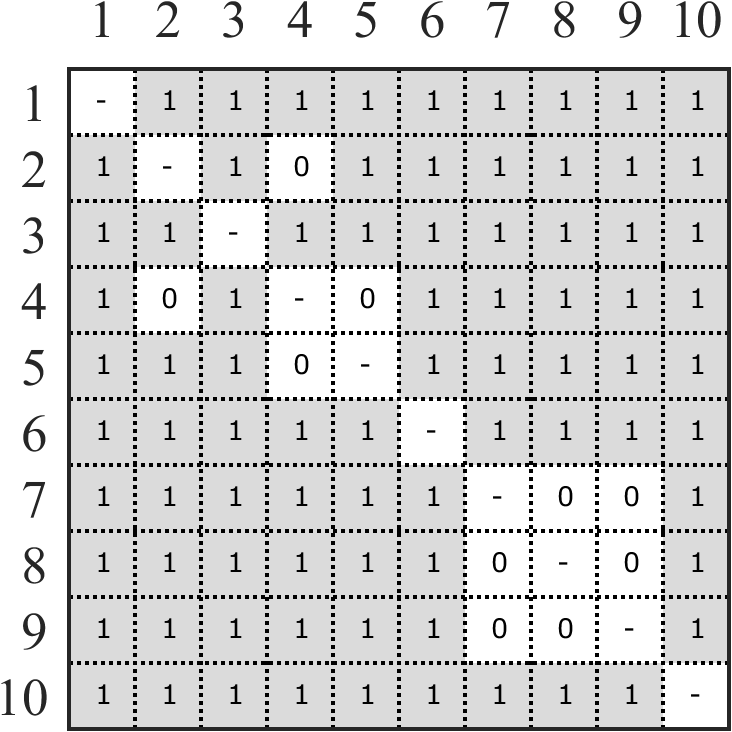
\includegraphics[scale=1]{meterTrack/bFmeas-statTest.png}
    } \hspace{0.1cm}
    \subfloat[\Gls{sama} f-measure ($\fmeas_s$)]{\label{fig:statTest:sfmeas}
      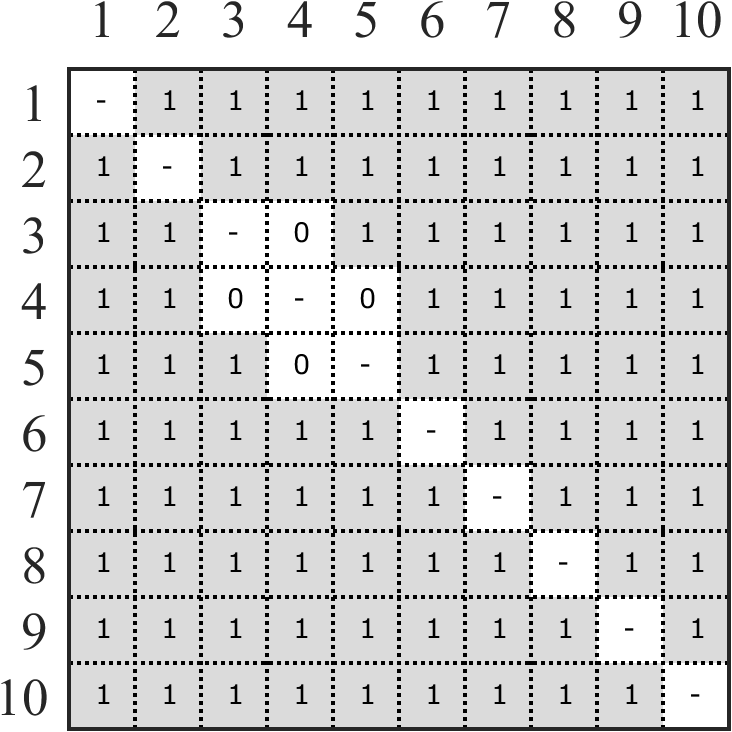
\includegraphics[scale=1]{meterTrack/sFmeas-statTest.png}
    }\\
    \subfloat[Beat $\amlt$ ($\amlt_{,b}$)]{\label{fig:statTest:bamlt}
      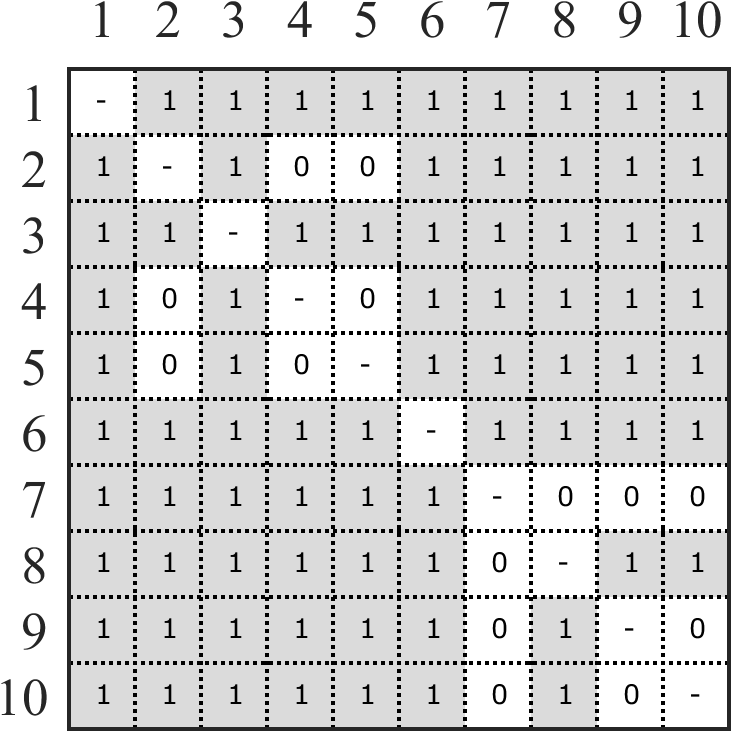
\includegraphics[scale=1]{meterTrack/bAMLt-statTest.png}
    } \hspace{0.1cm}
    \subfloat[Beat information Gain ($\infoGain_b$)]{\label{fig:statTest:binfogain}
      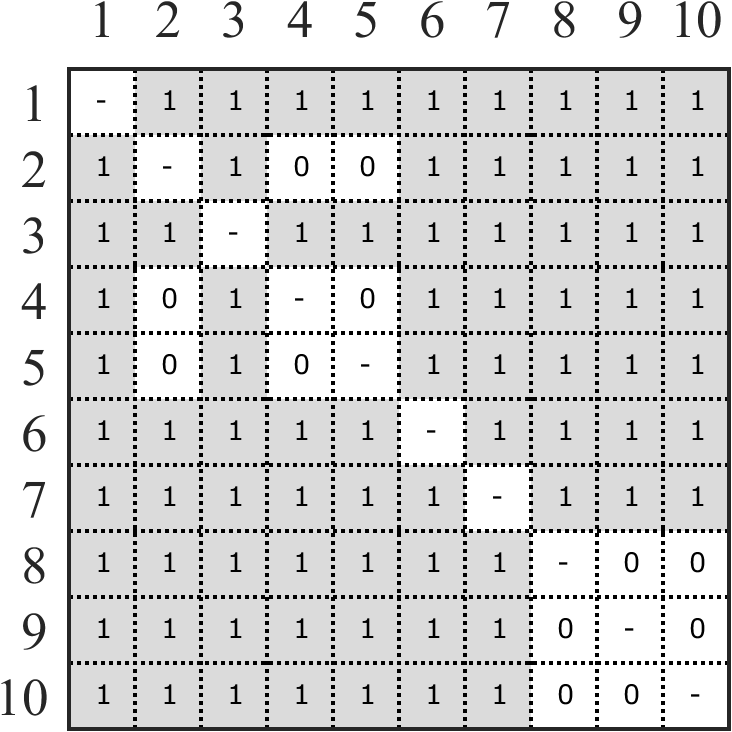
\includegraphics[scale=1]{meterTrack/bInfoGain-statTest.png}
    }
\caption[Results of statistical significance testing of meter analysis results on Indian art music datasets]{Results of statistical significance testing of meter analysis results on Indian art music datasets. The figure shows the results for the four different performance measures: Beat f-measure ($\fmeas_b$), \Gls{sama} f-measure ($\fmeas_s$), Beat $\amlt$ ($\amlt_{,b}$) and Beat information gain ($\infoGain_b$) in panels (a), (b), (c), and (d), respectively. For each measure, the figure shows the results of a pairwise statistical test between methods (algorithms) numbered 1-10 as a matrix. A gray box with numeral 1 indicates a statistically significant difference (at $p=0.05$) while a white box with numeral 0 indicates a difference that is not statistically significant. The methods 1-10 map to the ID shown in column-3 of \tabref{tab:resSummaryAll:IAM}.}\label{fig:statTest:all} %: 1 - Meter inference with \acrshort{hmmprior}, 2 - Meter inference with \acrshort{pfprior}, 3 - Meter tracking with \acrshort{hmmprior}, 4 - Meter tracking with \acrshort{pfprior}, 5 - Meter tracking with \acrshort{pfmix}, 6 - Meter tracking with \acrshort{pfsec}, 7 - Tempo-informed meter tracking with \acrshort{pfprior}, 8 - Tempo-informed meter tracking with \acrshort{pfsec}, 9 - Tempo-sama-informed meter tracking with \acrshort{pfprior}, 10 - Tempo-sama informed meter tracking with \acrshort{pfsec}.
\end{figure}  


A paired sample t-test with $p=0.05$ is used to assess statistically significant differences between the performances of algorithms. Statistical significance tests are done for the meter inference, meter tracking (including model extensions \momodel\ and \spmodel), and informed meter tracking methods by pooling the results over all Indian music datasets (\acrshort{CMDs}, \acrshort{HMDs}, \acrshort{HMDl} datasets - 269 pieces in total). Statistical significance tests are done for \bpmodel\ inference extensions (\acrshort{pfacc}, \acrshort{pfpkhop}, \acrshort{pfobshop}) by pooling the results over \acrshort{CMDs} and \acrshort{HMDs} (210 pieces in total) to compare with \acrshort{pfprior}.

We pool the results of meter inference, meter tracking (model extensions), tempo-informed tracking, and tempo-sama-informed tracking on all the Indian music datasets and present it in \tabref{tab:resSummaryAll:IAM}. The results of statistical significance tests between these approaches is presented in \figref{fig:statTest:all}. \tabref{tab:resSummaryAll:IAM} and \figref{fig:statTest:all} are to be analyzed in conjunction. In both the table and the figure, since $\nrhythmPatts=1$, note that \acrshort{pfmix} is equivalent to \acrshort{pfprior}. 

From \tabref{tab:resSummaryAll:IAM}, we see a consistent increase over the rows of the table across different meter analysis experiments (inference, tracking and informed tracking) indicating that incorporating additional prior information leads to improved meter analysis. Informed meter tracking has the best performance, while we see that meter tracking performance is mid-way between inference and informed meter tracking. 

The \figref{fig:statTest:all} shows that \acrshort{pfprior} and \acrshort{pfmix} are equivalent and produces results that are not statistically significantly different for all performance measures. The panel (a) in the figure for beat f-measure ($\fmeas_b$) shows that \acrshort{pfprior} algorithm in inference and tracking have statistically insignificant differences. In addition, \acrshort{pfprior} and \acrshort{pfsec} in tempo-informed tracking have insignificant differences with \acrshort{pfprior} in tempo-\gls{sama}-informed tracking. \Gls{sama} f-measure ($\fmeas_s$) shown in panel (b) indicates statistically insignificant differences between \acrshort{hmmprior} and \acrshort{pfprior}. 

The \spmodel\ shows statistically significant improvement over the methods that use \bpmodel\ indicating the use of section length shorter patterns for tracking downbeats. The significance results of beat $\amlt_{,b}$ measure in panel (c) is comparable to that for beat f-measure. Informed tracking methods have several statistically insignificant differences among themselves with the beat $\amlt_{,b}$ measure since the correct metrical level is already provided to the informed tracking algorithm, and hence leads to similar performance. An acceptable beat information gain ($\infoGain_b$ > 1.5 bits) is obtained in most cases, with several statistically insignificant differences in informed tracking. 

To summarize the results from \tabref{tab:resSummaryAll:IAM} and \figref{fig:statTest:all}, we see that informed tracking and algorithms using \spmodel\ improve \gls{sama} tracking performance significantly, while beat tracking performance also improves, but to a lesser extent. 

For an analysis and comparsion of inference extensions, we pool the results on Indian music datasets \acrshort{CMDs} and \acrshort{HMDs} and present it in \tabref{tab:resSummaryInfExt:IAM}. We compare the extensions \acrshort{pfacc}, \acrshort{pfpkhop} and \acrshort{pfobshop} with the baseline meter tracker \acrshort{pfprior}. In the table, since $\nrhythmPatts=1$, note that \acrshort{pfacc} is equivalent to \acrshort{pfprior}. Statistical tests indicate that for all measures, \acrshort{pfprior} and \acrshort{pfacc} are equivalent and show no statistically significant difference in performance. In addition, for all measures, \acrshort{pfpkhop} and \acrshort{pfobshop} both give significantly lower performance compared to \acrshort{pfprior}. The hop inference extensions need further improvement and do not match up to the performance of doing a full inference at every frame. % The results of statistical significance tests between these approaches is presented in \figref{fig:statTestInfExt:all}. \tabref{tab:resSummaryInfExt:IAM} and \figref{fig:statTestInfExt:all} are to be analyzed in conjunction.
%% The small table of inference extensions
\begin{table}
\setlength{\tabcolsep}{1.5\tabcolsep}
\centering
 \begin{tabular}{@{}LCCCCCCCCC@{}} \toprule
Algo. &ID& $\fmeas_b$ & $\amlt_{,b}$ & $\infoGain_b$ && $\fmeas_{s}$ && \multicolumn{2}{c}{Tempo} \tabularnewline 
&& & & Bits && && \gls{CML} & \gls{AML} \tabularnewline \midrule 
\acrshort{pfprior} &1& 0.852 & 0.848 & 1.83 && 0.715 && 0.90 & 0.97 \tabularnewline \addlinespace[3pt]
\acrshort{pfacc} &2& 0.850 & 0.849 & 1.82 && 0.716 && 0.90 & 0.97 \tabularnewline 
\acrshort{pfpkhop} &3& 0.579 & 0.566 & 0.63 && 0.240 && 0.85 & 0.93 \tabularnewline 
\acrshort{pfobshop} &4& 0.784 & 0.761 & 1.40 && 0.612 && 0.85 & 0.94 \tabularnewline \bottomrule
\end{tabular}
\caption[Summary of meter tracking performance of inference extensions]{Summary of meter tracking performance of inference extensions on \acrshort{CMDs} and \acrshort{HMDs} datasets. The second column shows the different algorithms. The table shows the tempo estimation performance at \gls{CML} and \gls{AML}, beat and \gls{sama} (downbeat) tracking performance with different measures.}\label{tab:resSummaryInfExt:IAM} % The column ID on second column corresponds to the labels used in \protect\figref{fig:statTestInfExt:all}, which shows the results of statistical significance tests on these results.
\end{table}
%% The small table of R=2
\begin{table}[t]
\setlength{\tabcolsep}{1.5\tabcolsep}
\centering
 \begin{tabular}{@{}LCCCCCCCCC@{}} \toprule
Algo. && $\fmeas_b$ & $\amlt_{,b}$ & $\infoGain_b$ && $\fmeas_{s}$ && \multicolumn{2}{c}{Tempo} \tabularnewline 
&& & & Bits && && \gls{CML} & \gls{AML} \tabularnewline \midrule 
\acrshort{pfprior} && 0.735 & 0.751 & 1.68 && 0.641 && 0.77 & 0.88 \tabularnewline \addlinespace[3pt]
\acrshort{pfmix} && \textbf{0.749} & \textbf{0.773} & \textbf{1.75} && 0.660 && 0.78 & 0.89 \tabularnewline \bottomrule
\end{tabular}
\caption[Comparing the meter tracking performance of \acrshort{pfprior} and \acrshort{pfmix} algorithms]{Comparing the meter tracking performance of \acrshort{pfprior} and \acrshort{pfmix} algorithms on Indian art music datasets for $\nrhythmPatts=2$ patterns. Numbers in bold for the beat and \gls{sama} tracking measures indicate a statistically significant improvement.}\label{tab:trackRtwo:AMPFoAMPFm}
\end{table}

With that summary of results, we now focus on some more analysis with $\nrhythmPatts = 2$ comparing meter tracking performance of \acrshort{pfprior} with \acrshort{pfmix} and \acrshort{pfacc}.  \tabref{tab:trackRtwo:AMPFoAMPFm} shows a summary of results over all the Indian music datasets for meter tracking with \acrshort{pfprior} and \acrshort{pfmix} and $\nrhythmPatts = 2$. An analysis showed that there is no statistically significant difference in results between $\nrhythmPatts = 1$ and $\nrhythmPatts = 2$ for either \acrshort{pfprior} or \acrshort{pfmix} (for all measures). However, for $\nrhythmPatts = 2$, the beat tracking measures show an improvement for \acrshort{pfmix} over \acrshort{pfprior}. For the case of \acrshort{pfacc} compared with \acrshort{pfprior} however, there was no statistically significant improvement with more patterns, showing the need for further exploration of the end-of-bar sampling \gls{AMPF} algorithm to improve its performance. 
% \comment{Place to do final set of inferences from experiments, and conclusions}
\section{Conclusions}
We defined different meter analysis tasks within the context of Indian art music, pointing out the distinctions between meter inference, meter tracking and informed meter tracking. After a set of preliminary experiments on Carnatic music, we explored Bayesian models for jointly tracking several aspects of meter. The state of the art bar pointer model was presented, and several model and inference extensions were proposed to improve meter analysis. 

An extensive evaluation of different meter analysis models and algorithms was discussed for different Indian art music datasets, with Ballroom dataset results reported for comparison. Indian art music, with complex metrical structures is an ideal case to study the performance of novel methods for meter analysis and hence such an evaluation is valuable to improve state of the art in meter tracking in \gls{MIR}. %To the best of our knowledge, the work in this chapter is the first collective and comprehensive work on meter analysis in Carnatic and Hindustani music. 

The Bayesian models explicitly considered musically relevant information for meter analysis, leading to culture-aware algorithms. However, the algorithms and models are flexible and can easily adapt to cyclical metrical structures in other music cultures such as Turkish makam music (\textit{usul}) and to Arab-andalusian music (\textit{mîzân}). Such Bayesian machine learning models require a small amount of beat and downbeat annotated training data from which we can learn these models and build specific algorithms. Exploring such extensions to different music cultures is one of the goals of future work in the area. 

The \spmodel\ shows significant promise in automatic meter analysis. It is a flexible model that can track any cyclical metrical structure by tracking smaller meaningful sub-patterns of the cycle. It provides a significant improvement with Indian music, and it would be fruitful to explore it further in other music cultures. It additionally goes on to show that tracking shorter length patterns is useful for tracking long duration metrical structures, an intuitive conclusion considering that several additive meters are tracked that way. 

The results were mostly reported on the \acrshort{CMDs}, \acrshort{HMDs}, and \acrshort{HMDl} datasets that consist of two minute long pieces. However, as reported by \citeA{ajay:15:pf} and as seen from additional experiments, these algorithms extend to full length pieces in Carnatic music, showing an equivalent performance. While computational complexity is one factor for meter analysis in full length pieces, there can be several ways in which it can be reduced and the approaches described in the chapter can be applied. A future evaluation on a larger dataset with full length pieces, such as the rhythm annotated pieces in \acrshort{HMDo} and \acrshort{CMDo} collections will further boost such a claim. 

One main limitation of the algorithms presented in the chapter was the assumption of a single \gls{tala} for the whole audio recording presented to the algorithm. While this is a fair and realistic assumption for Carnatic music, which is distributed as segmented recordings containing a single piece, Hindustani music recordings can have two or more pieces in different \gls{taal} and \gls{lay}. A rhythm based segmentation might be necessary there before applying the meter analysis algorithms. Such segmentation could be performed using, e.g. Bayesian change point detection \cite{barber:11:bayesian}, a problem that needs further exploration.

The approaches in the chapter utilized bar/section length rhythm patterns for meter tracking. Indian art music is replete with several rhythmic patterns and hence should benefit algorithms that use multiple patterns to model a cycle. However, the experiments did not show such an improvement. There was no statistically significant improvement observed with additional rhythmic patterns ($\nrhythmPatts > 1$). This can be primarily attributed the simplistic \gls{GMM} based observation model and the spectral flux based feature that fail to capture nuances from multiple patterns and model them effectively. Better features that can capture nuances and a better observation model need to explored to utilize the variability in patterns we encounter in Indian art music and use them for meter analysis. 

\Gls{vilambit} (slow tempo) pieces in Hindustani music pose a significant challenge for meter tracking. They are further a challenge for evaluating a meter tracker output. During the rendering of metrical cycles as long as a minute, the \glspl{matra} within the cycle are quite flexibly rendered with expressive timing. In addition, given the large inter-\gls{matra} interval, larger errors in tracking are acceptable for listeners. However, the \gls{matra} at the beginning and end of the cycle are more important to keep the time and hence have to be more accurate. An evaluation measure that treats all the beats of an output as the same is not the best evaluation measure for such a case. The standard evaluation measures considered in the thesis, including the continuity measures $\cmlt$ and $\amlt$, cannot handle such cases where there needs to different weights on errors depending on metrical position and tempo. In the evaluation of \acrshort{HMDl} pieces in this chapter, we used 6.25\% of the median inter-\gls{matra} interval as the error window for all \gls{matra} of the piece. Though it allows for more flexibility in evaluation of long duration metrical cycles, better measures that can consider the metrical position might be more meaningful. Such measures are to be further developed and tested to reflect a more accurate measure of performance of the meter tracking algorithms from a listener's perspective. 

A comparison across different \glspl{tala} showed that longer \glspl{tala} that have a higher diversity of patterns played in them are more difficult to track, e.g. \gls{adi} \gls{tala} in Carnatic music. \Gls{vilambit} \gls{ektal} in Hindustani music is also difficult to track owing to its long duration cycles and equal length \glspl{vibhaag}. The section length rhythmic patterns in \gls{ektal} are equal in length and similar, which is confusing to a tracker that uses only spectral energy based features. In summary, longer \glspl{tala} that have wider scope for improvisation are difficult to track, with longer duration cycles adding further to tracking complexity. 

Apart from the percussion patterns played on mridangam and \gls{tabla} that are indicative of the position in metrical cycle, in many cases, melodic patterns also indicate the position in cycle. This is further true in compositional forms of both Hindustani and Carnatic music, which are composed in a specific \gls{tala}. Melody also can be used to track the progression through a \gls{tala} with several melodic and lyrical markers indicating the \gls{sama}. Incorporating melody and lyrics based features into the observation model is hence hypothesized to additionally help to improve meter analysis performance. 

The presented Bayesian models can be further improved to incorporate other structures and priors that can be utilized for improving meter tracking - such as tighter bounds on tempo, tighter restriction on continuity, and allowance for errors such a skipping a beat. This is in addition to the ideas explored already: such as hop inference that aims to track meter only at specific event cues. Such models need to be further explored, with suitable and efficient inference algorithms. The computationally efficient mixture observation model and the inference extensions presented in the chapter show some promise, but need further improvement. They can be better utilized with more rhythmic patterns modeling a \gls{tala}, which needs more diverse features. The use of better features and faster inference with better models can be a focus in future research on the topic. Recent approaches that use deep learning to build observation models have also seen some success~\cite{bock:11:nnbeat}, motivating us to explore them further. 

The meter analysis algorithms discussed in the chapter were developed within the context of CompMusic project and hence are aligned with its goals to lead towards defining relevant rhythm similarity measures. Meter analysis is the first step towards that goal. Automatic meter analysis provides valuable content based metadata for a piece of music with several useful applications: a few of them are detailed in \chapref{chap:conclusions}. 
% 
% 
% \begin{figure}
% \centering
%     \subfloat[Beat f-measure ($\fmeas_b$)]{\label{fig:statTestInfExt:bfmeas}
%       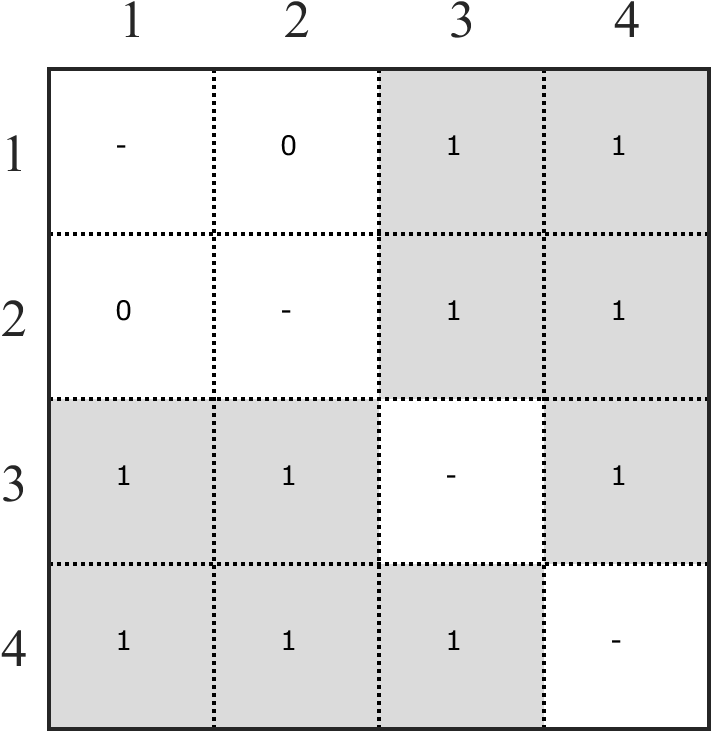
\includegraphics[scale=1]{meterTrack/bFmeas-statTest-infExt.png}
%     } \hspace{0.1cm}
%     \subfloat[\Gls{sama} f-measure ($\fmeas_s$)]{\label{fig:statTestInfExt:sfmeas}
%       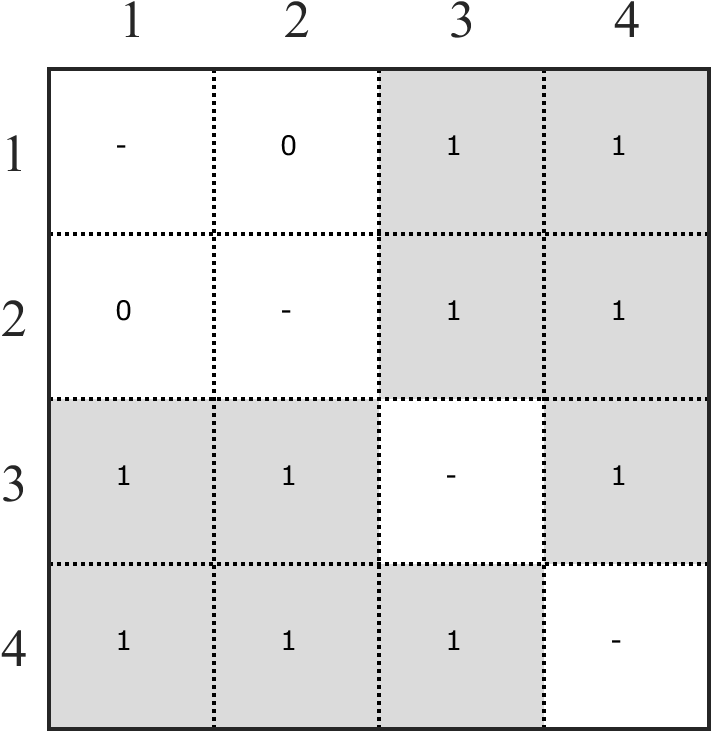
\includegraphics[scale=1]{meterTrack/sFmeas-statTest-infExt.png}
%     }\\
%     \subfloat[Beat $\amlt$ ($\amlt_{,b}$)]{\label{fig:statTestInfExt:bfmeas}
%       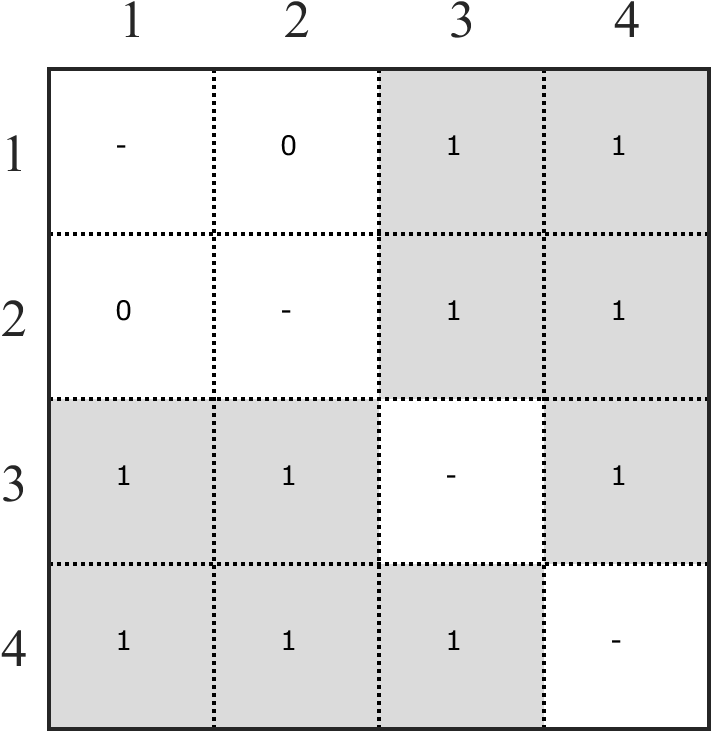
\includegraphics[scale=1]{meterTrack/bAMLt-statTest-infExt.png}
%     } \hspace{0.1cm}
%     \subfloat[Beat information Gain ($\infoGain_b$)]{\label{fig:statTestInfExt:sfmeas}
%       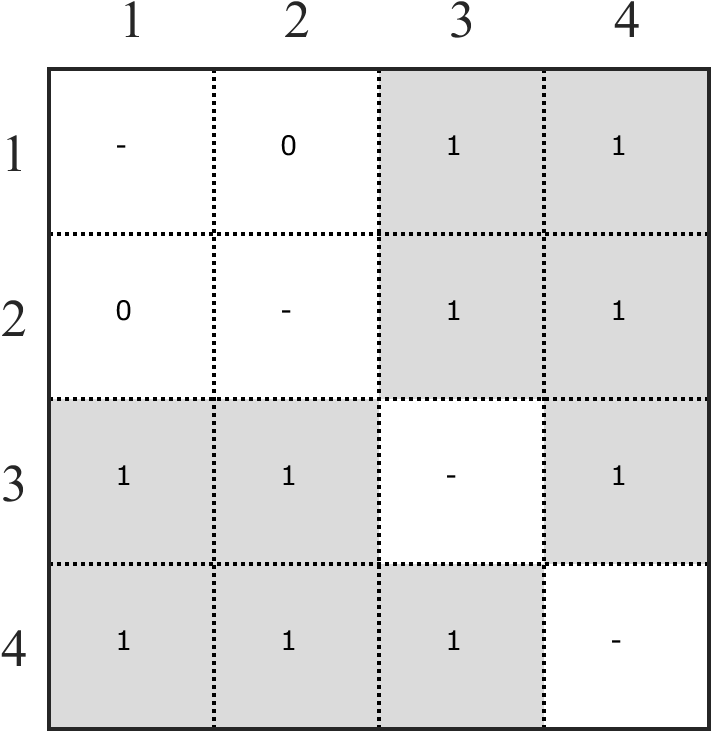
\includegraphics[scale=1]{meterTrack/bInfoGain-statTest-infExt.png}
%     }
% \caption[Results of statistical significance testing of meter tracking results for inference extensions]{Results of statistical significance testing of meter tracking results for inference extensions. The figure shows the results for the four different performance measures: Beat f-measure ($\fmeas_b$) in panel (a), \Gls{sama} f-measure ($\fmeas_s$) in panel (b), Beat $\amlt$ ($\amlt_{,b}$) in panel (c), and Beat information Gain ($\infoGain_b$) in panel (d). For each measure, the figure shows the results of a pairwise statistical test between methods (algorithms) numbered 1-4 as a matrix. A gray box with numeral 1 indicates a statistically significant difference ($p=0.05$) while a box with numeral 0 indicates a difference that is not statistically significant. The meter tracking methods 1-4 map to the ID shown in \tabref{tab:resSummaryInfExt:IAM}: 1 - \acrshort{pfprior}, 2 - \acrshort{pfacc}, 3 - \acrshort{pfpkhop}, 4 - \acrshort{pfobshop}.}\label{fig:statTestInfExt:all}
% \end{figure}
%
% 
%
% With a wide range of tempo, cycles as long as a minute, and non-isochronous subdivisions of the cycle, Hindustani music is a suitable case to experiment with for extending the horizon of the state of the art in meter tracking \cite{ajay:14:rhythmJNMR}. There has been some previous work in rhythmic analysis of Hindustani music in meter estimation \cite{sankalp:12:meter} and \gls{taal} recognition \cite{miron:11:thesis}, but to the best of our knowledge, this is the first work to propose meter tracking for Hindustani music.
% 
%
%\note{Problem description and different levels, recap}
%\begin{enumerate}
%\item Meter Inference: Estimate meter type, tempo, beats, sections, and downbeats, all together...
%\item Meter Tracking: Given meter type, estimate tempo, beats, sections, and downbeats, all together... (most relevant)
%\item Tempo informed meter tracking: Given the meter type and a ``tight" tempo range, estimate tempo, beats, sections, and downbeats. Mainly to see the effects of tempo on tracking performance.  
%\item Tempo + \gls{sama} informed tracking: Given the meter type, a ``tight" tempo range and the first instance of the downbeat, estimate tempo, beats, sections, and downbeats.
%\item Downbeat tracking: Given all the beat positions (and indirectly the tempo, and the meter type), estimate the downbeat. Not a relevant problem. 
%\item Beat Tracking: Relevant, but ill defined. 
%\end{enumerate}
%
%\note{Explain which of these problems are addressed in the thesis: Mainly Meter tracking, but also some expts on tempo informed meter tracking and meter inference. Methods: Preliminary experiments based on DP and features, followed by Bayesian Models. Evaluations are provided on CMD (all), CMDf(some), HMDf (some), HMDs (some), HMDl (some).}

%\note{Model structure: The bar pointer model (classic), the simplified bar pointer model (ISMIR 2015), the section pointer model (ICASSP 2016, submitted). Explain how they can be used for meter inference, what do the different variants signify, and what assumptions they make.}
%\note{Priors: How tempo informed tracking works exactly}
%\note{Transition Model: No trans, prior trans, fixed trans for patterns, Tempo transitions: The way it depends on ranges now}
%\note{Observation model: Regular, mixture observation model, and gated observation model}
%\note{All presented in a sequence, have to organize this better once all the results are compiled and present.}
%\comment{HMM results (ISMIR 2014): CMD, TMD, Cretan, Ballroom refer to Florian's work}
%\comment{AMPF\_obs results on Carnatic music (ISMIR 2015): CMDx, Ballroom dataset}
%\comment{SPM extensions on Carnatic and Hindustani music (ICASSP 2016): HMDx, CMDx (to be run)}
%\comment{Additional expts: Tempo informed tracking, comparison of performance}
%\dtext{Journal paper material here: Gated observation model, full section pointer model, evaluations on Indian music, Cretan music, Turkish music.}
%\comment{Mainly DBNs, that track different aspects of meter. Bayesian models: Formulation and inference in detail, HMM and PF variants.}
%%% Canonical forms of results tables
% \begin{table}
% \centering
% \begin{tabular}{@{}llcccccccc@{}}
% \toprule 
% & Measure & \multicolumn{2}{c}{\fmeas} && \multicolumn{2}{c}{\amlt} && \multicolumn{2}{c}{\infoGain}\tabularnewline 
% & \nrhythmPatts & 1 & 2 && 1 & 2 && 1 & 2\tabularnewline
% \midrule 
% \multirow{5}{*}{\rotatebox[origin=c]{90}{Sama}} & \Gls{adi} & 0.893 & 0.893 && 0.893 & 0.893 && 2.89 & 2.89\tabularnewline
% & \Gls{rupaka} &  0.893 & 0.893 && 0.893 & 0.893 && 2.89 & 2.89\tabularnewline
% & \Gls{mishra chapu} &  0.893 & 0.893 && 0.893 & 0.893 && 2.89 & 2.89\tabularnewline
% & \Gls{khanda chapu} &  0.893 & 0.893 && 0.893 & 0.893 && 2.89 & 2.89\tabularnewline \addlinespace[2pt]
% & \textbf{Mean} &  \textbf{0.893} & \textbf{0.893} && \textbf{0.893} & \textbf{0.893} && \textbf{2.89} & \textbf{2.89}\tabularnewline
% \midrule 
% \multirow{5}{*}{\rotatebox[origin=c]{90}{Beat}} & \Gls{adi} & 0.893 & 0.893 && 0.893 & 0.893 && 2.89 & 2.89\tabularnewline
% & \Gls{rupaka} &  0.893 & 0.893 && 0.893 & 0.893 && 2.89 & 2.89\tabularnewline
% & \Gls{mishra chapu} &  0.893 & 0.893 && 0.893 & 0.893 && 2.89 & 2.89\tabularnewline
% & \Gls{khanda chapu} &  0.893 & 0.893 && 0.893 & 0.893 && 2.89 & 2.89\tabularnewline \addlinespace[2pt]
% & \textbf{Mean} &  \textbf{0.893} & \textbf{0.893} && \textbf{0.893} & \textbf{0.893} && \textbf{2.89} & \textbf{2.89}\tabularnewline
% \bottomrule
% \end{tabular}
% \protect\caption{test 1 test 2 test 3 test 4. test 1 test 2 test 3 test 4. test 1 test 2 test 3 test 4. test 1 test 2 test 3 test 4. test 1 test 2 test 3 test 4. test 1 test 2 test 3 test 4.  test 1 test 2 test 3 test 4. }\label{tab:canon:result1}
% \end{table}
% 
% \begin{table}
% \centering
% \begin{tabular}{@{}llcccccccc@{}} \toprule
%  & Measure & \multicolumn{2}{c}{\fmeas} && \multicolumn{2}{c}{\amlt} && \multicolumn{2}{c}{\infoGain}\tabularnewline \addlinespace[2pt]
%  & $\nrhythmPatts$ & 1 & 2 && 1 & 2 && 1 & 2\tabularnewline \midrule
% \multirow{5}{*}{\rotatebox[origin=c]{90}{\Gls{sama}}} & \Gls{adi} & 1.634 & 2.634 && 1.922 & 2.922 && 5.58 & 6.58\tabularnewline
%  & \Gls{rupaka} & 1.804 & 2.804 && 1.967 & 2.967 && 5.21 & 6.21\tabularnewline
%  & \Gls{mishra chapu} & 1.930 & 2.930 && 1.984 & 2.984 && 5.46 & 6.46\tabularnewline
%  & \Gls{khanda chapu} & 1.868 & 2.868 && 1.958 & 2.958 && 5.03 & 6.03\tabularnewline \addlinespace[2pt]
%  & \textbf{Mean} & \textbf{1.808} & \textbf{2.808} && \textbf{1.958} & \textbf{2.958} && \textbf{5.32} & \textbf{6.32}\tabularnewline \midrule
% \multirow{5}{*}{\rotatebox[origin=c]{90}{Beat}} & \Gls{adi} & 1.808 & 2.808 && 1.958 & 2.958 && 5.32 & 6.32\tabularnewline
%  & \Gls{rupaka} & 1.796 & 2.796 && 1.933 & 2.933 && 3.46 & 4.46\tabularnewline
%  & \Gls{mishra chapu} & 1.864 & 2.864 && 1.973 & 2.973 && 3.85 & 4.85\tabularnewline
%  & \Gls{khanda chapu} & 1.943 & 2.943 && 1.936 & 2.936 && 2.97 & 3.97\tabularnewline \addlinespace[2pt]
%  & \textbf{Mean} & \textbf{1.892} & \textbf{2.892} && \textbf{1.950} & \textbf{2.950} && \textbf{3.33} & \textbf{4.33}\tabularnewline \bottomrule
% \end{tabular}
% \caption[tempo-informed tracking with AMPF-prior-allHop-bar on \acrshort{CMDs} dataset]{Results of tempo-informed tracking with AMPF-prior-allHop-bar on \acrshort{CMDs} dataset}
% \end{table}
% 
% \begin{table}
% \centering
% \begin{tabular}{@{}lcccccccc@{}}
% \toprule 
% Measure & \multicolumn{2}{c}{\fmeas} && \multicolumn{2}{c}{\amlt} && \multicolumn{2}{c}{\infoGain}\tabularnewline \addlinespace[2pt]
% $\nrhythmPatts$ & 1 & 2 && 1 & 2 && 1 & 2\tabularnewline
% \midrule 
% Sama Tracking &  0.893 & 0.893 && 0.893 & 0.893 && 2.89 & 2.89\tabularnewline \addlinespace[3pt]
% Beat Tracking &  0.893 & 0.893 && 0.893 & 0.893 && 2.89 & 2.89\tabularnewline
% \bottomrule
% \end{tabular}
% \protect\caption{test 1 test 2 test 3 test 4. test 1 test 2 test 3 test 4. test 1 test 2 test 3 test 4. test 1 test 2 test 3 test 4. test 1 test 2 test 3 test 4. test 1 test 2 test 3 test 4.  test 1 test 2 test 3 test 4. }\label{tab:canon:allresults}
% \end{table}
% 
% \begin{table}
% \centering
% \begin{tabular}{@{}lcccccccc@{}} \toprule
% Measure & \multicolumn{2}{c}{\fmeas} && \multicolumn{2}{c}{\amlt} && \multicolumn{2}{c}{\infoGain}\tabularnewline \addlinespace[2pt]
% $\nrhythmPatts$ & 1 & 2 && 1 & 2 && 1 & 2\tabularnewline \midrule
% \Gls{sama} Tracking & 1.808 & 2.808 && 1.958 & 2.958 && 5.32 & 6.32\tabularnewline \addlinespace[3pt] 
%  Beat Tracking & 1.892 & 2.892 && 1.950 & 2.950 && 3.33 & 4.33\tabularnewline \bottomrule
% \end{tabular}
% \caption[tempo-informed tracking with AMPF-prior-allHop-bar on \acrshort{CMDs} dataset]{Results of tempo-informed tracking with AMPF-prior-allHop-bar on \acrshort{CMDs} dataset}
% \end{table}
%
%Global settings for experiments
%\begin{itemize}
	%\item Two fold cross validation, mean over three runs
	%\item All tempo ranges are learned from training data, with 20\% margin allowed on learned ranges.  % Move to expts section: In this thesis, we assume uniform priors on all variables, within the allowed ranges of tempo. In the dissertation, for the meter inference and tracking tasks, we learn the tempo ranges directly from training data. 
	%\item HMM parameter values list
	%\item PF parameter values list 
	%\item %Results reported as mean over all rhythm classes for each dataset. A final summary of results over all datasets is also presented. 
	%\item %Meter Inference results are presented first. Followed by meter tracking: model and inference extensions. Tempo informed tracking and Tempo-sama informed tracking results follow next. 
	%\item %Evaluation: b-Fmeas ($\fmeas_b$), b-AMLt ($\amlt_{,b}$), b-infoGain ($\infoGain_b$), s-Fmeas ($\fmeas_s$) are used. Fmeas computed using 70 ms window for \acrshort{CMDs}, \acrshort{HMDs}, and Ballroom datasets - smaller cycles. But for \acrshort{HMDl}, a bigger margin window is allowed since cycles are very long and current BT evaluation approaches were not designed with such long cycles in mind, 70ms is very tight. To account for the length of the cycle in the margin, a 6.25\% median inter annotation interval is used as margin, as used in many beat tracking evaluations. This corroborates well with vilambit pieces since there can be significant freedom in pulsation, and also that larger errors also are unnoticed since the pieces are not rhythmically dense. The pulsation is also beyond the duration of perceptual present. 
	%\item %For evaluating median tempo estimation performance, we compare the median estimated tempo and the median annotated ground truth tempo with a 5\% margin. We compute both CML and AML accuracy. AML assumes a tempo scaling by 0.25, 0.5, 1, 2, 4 to be correct. Tala recognition accuracy is also reported for meter inference. 
%\end{itemize}
% The tempo ranges $[\dot{\phi}_{\textrm{min}}, \dot{\phi}_{\textrm{max}}]$ are learned from the training data of each fold, with an additional 20\% margin for unseen data. For the SPM, the length of longest section, $M=1600$, is set for the four \gls{matra} long sections in \gls{teental} and other section lengths are scaled accordingly. The number of particles is set equal to $N_p=1500\cdot V$. For the BPM hence, since $V=1$, $M=1600$ corresponds to the whole of the longest cycle(\gls{teental}) and $N_p=1500$. For the AMPF, we set $\sigma_n = 0.02$ and the maximum number clusters to 200. The other AMPF parameters are identical to the values used in \cite{Krebs2014:pf}.
% 
% The tempo ranges were manually set for Carnatic music as $\dot{\phi} \in [4,15]$ (cycle lengths between 1.33\,s and 8\,s) and $\dot{\phi} \in [6,32]$ (bar lengths between 0.75\,s to 5.3\,s) for the Ballroom dataset. With $M_{\mathrm{max}} = 1600$ (corresponds to \gls{adi} \gls{tala} with 8 beats/cycle), the length of cycle $M$ and the number of beats $B$ for each \gls{tala} is shown in~\tabref{tab:dataset}. For Ballroom dataset, we used $M=1600$ and $M=1200$ for tracking time signatures 4/4 and 3/4, respectively. For the HMM, we use $p_n=0.02$ as in~\cite{krebs:13:bpm}, and for the AMPF, we use $\sigma_{\dot\phi}=10^{-4}\cdot M$. We explore the performance with $R = \{1,2,4\}$, with the number of particles set to $N_p=1500 \cdot R$. The other AMPF parameters are identical to the values used in \cite{Krebs2014:pf}.
%
% \begin{itemize}
% 	% \item Results presented only for $R=1$. $R=2$ does not show much improvement. When necessary, performance with $R=2$ is indicated. With $R=1$, model extension \acrshort{pfmix} and inference extension \acrshort{pfacc} are equivalent to the baseline \acrshort{pfprior}. 
% 	% \item Results specific to each tala/rhythm class are discussed when needed in text. 
% 	% \item Also, all the meter tracking experiments on Hindustani music are not just tala informed, but also lay (tempo class) informed, i.e. the algorithm knows if it is tracking long cycles or short cycles. 
% 	%\item Performance on ballroom dataset is shown for meter inference and tracking tasks. 
% 	\item Inference extensions are only evaluated on \acrshort{CMDs} and \acrshort{HMDs} datasets (Ballroom dataset shown for reference) and compared with \acrshort{pfprior}. Statistical significance tests are done for inference extensions (\acrshort{pfacc}, \acrshort{pfpkhop}, \acrshort{pfobshop}) by pooling the results over \acrshort{CMDs} and \acrshort{HMDs} (210 pieces in total) to compare with \acrshort{pfprior}. 
% 	\item Statistical significance tests are done for all the inference, tracking (model extensions), and informed tracking methods by pooling the results over all Indian music datasets (\acrshort{CMDs}, \acrshort{HMDs}, \acrshort{HMDl} - 269 pieces in total).
% 	\item A paired sample t-test with p=0.05 is used to assess statistically significant differences. 
% \end{itemize} 
%
%
%
%
% \note{\textit{Chapter in brief: The main chapter of the thesis discussing meter inference and tracking, first with traditional signal processing approaches and later on with Bayesian models using HMM and PF inference schemes. Present and discuss several models applied to both Carnatic and Hindustani music datasets, with additional evaluation on ballroom dataset and Turkish datasets. The chapter is comprehensive and needs to discuss several results coherently. It will include some future work in the form of gated observation model and the grand unified journal paper results. The material for the chapter are from ISMIR 2014, ICASSP 2014, ISMIR 2015, ICASSP’16, and the journal paper under preparation.}}
%
%The \gls{taal} cycle is the largest regularly repeating time unit;
  %\qitem{... when a mridangam player accompanies a musician (vocalist or instrumentalist) in India, he [/she] does not merely beat the sarva laghu [standard rhythm patterns], but provides a cross-rhythmical accompaniment based on style, movement and rhythmical construction of the pieces rendered.}{\citeA[Book II, p. 18]{samba:98:southMusic} \\ \emph{Text in brackets by the author.}}